% Options for packages loaded elsewhere
\PassOptionsToPackage{unicode}{hyperref}
\PassOptionsToPackage{hyphens}{url}
\PassOptionsToPackage{dvipsnames,svgnames,x11names}{xcolor}
%
\documentclass[
  letterpaper,
  DIV=11,
  numbers=noendperiod]{scrreprt}

\usepackage{amsmath,amssymb}
\usepackage{iftex}
\ifPDFTeX
  \usepackage[T1]{fontenc}
  \usepackage[utf8]{inputenc}
  \usepackage{textcomp} % provide euro and other symbols
\else % if luatex or xetex
  \usepackage{unicode-math}
  \defaultfontfeatures{Scale=MatchLowercase}
  \defaultfontfeatures[\rmfamily]{Ligatures=TeX,Scale=1}
\fi
\usepackage{lmodern}
\ifPDFTeX\else  
    % xetex/luatex font selection
\fi
% Use upquote if available, for straight quotes in verbatim environments
\IfFileExists{upquote.sty}{\usepackage{upquote}}{}
\IfFileExists{microtype.sty}{% use microtype if available
  \usepackage[]{microtype}
  \UseMicrotypeSet[protrusion]{basicmath} % disable protrusion for tt fonts
}{}
\makeatletter
\@ifundefined{KOMAClassName}{% if non-KOMA class
  \IfFileExists{parskip.sty}{%
    \usepackage{parskip}
  }{% else
    \setlength{\parindent}{0pt}
    \setlength{\parskip}{6pt plus 2pt minus 1pt}}
}{% if KOMA class
  \KOMAoptions{parskip=half}}
\makeatother
\usepackage{xcolor}
\setlength{\emergencystretch}{3em} % prevent overfull lines
\setcounter{secnumdepth}{5}
% Make \paragraph and \subparagraph free-standing
\ifx\paragraph\undefined\else
  \let\oldparagraph\paragraph
  \renewcommand{\paragraph}[1]{\oldparagraph{#1}\mbox{}}
\fi
\ifx\subparagraph\undefined\else
  \let\oldsubparagraph\subparagraph
  \renewcommand{\subparagraph}[1]{\oldsubparagraph{#1}\mbox{}}
\fi

\usepackage{color}
\usepackage{fancyvrb}
\newcommand{\VerbBar}{|}
\newcommand{\VERB}{\Verb[commandchars=\\\{\}]}
\DefineVerbatimEnvironment{Highlighting}{Verbatim}{commandchars=\\\{\}}
% Add ',fontsize=\small' for more characters per line
\usepackage{framed}
\definecolor{shadecolor}{RGB}{241,243,245}
\newenvironment{Shaded}{\begin{snugshade}}{\end{snugshade}}
\newcommand{\AlertTok}[1]{\textcolor[rgb]{0.68,0.00,0.00}{#1}}
\newcommand{\AnnotationTok}[1]{\textcolor[rgb]{0.37,0.37,0.37}{#1}}
\newcommand{\AttributeTok}[1]{\textcolor[rgb]{0.40,0.45,0.13}{#1}}
\newcommand{\BaseNTok}[1]{\textcolor[rgb]{0.68,0.00,0.00}{#1}}
\newcommand{\BuiltInTok}[1]{\textcolor[rgb]{0.00,0.23,0.31}{#1}}
\newcommand{\CharTok}[1]{\textcolor[rgb]{0.13,0.47,0.30}{#1}}
\newcommand{\CommentTok}[1]{\textcolor[rgb]{0.37,0.37,0.37}{#1}}
\newcommand{\CommentVarTok}[1]{\textcolor[rgb]{0.37,0.37,0.37}{\textit{#1}}}
\newcommand{\ConstantTok}[1]{\textcolor[rgb]{0.56,0.35,0.01}{#1}}
\newcommand{\ControlFlowTok}[1]{\textcolor[rgb]{0.00,0.23,0.31}{#1}}
\newcommand{\DataTypeTok}[1]{\textcolor[rgb]{0.68,0.00,0.00}{#1}}
\newcommand{\DecValTok}[1]{\textcolor[rgb]{0.68,0.00,0.00}{#1}}
\newcommand{\DocumentationTok}[1]{\textcolor[rgb]{0.37,0.37,0.37}{\textit{#1}}}
\newcommand{\ErrorTok}[1]{\textcolor[rgb]{0.68,0.00,0.00}{#1}}
\newcommand{\ExtensionTok}[1]{\textcolor[rgb]{0.00,0.23,0.31}{#1}}
\newcommand{\FloatTok}[1]{\textcolor[rgb]{0.68,0.00,0.00}{#1}}
\newcommand{\FunctionTok}[1]{\textcolor[rgb]{0.28,0.35,0.67}{#1}}
\newcommand{\ImportTok}[1]{\textcolor[rgb]{0.00,0.46,0.62}{#1}}
\newcommand{\InformationTok}[1]{\textcolor[rgb]{0.37,0.37,0.37}{#1}}
\newcommand{\KeywordTok}[1]{\textcolor[rgb]{0.00,0.23,0.31}{#1}}
\newcommand{\NormalTok}[1]{\textcolor[rgb]{0.00,0.23,0.31}{#1}}
\newcommand{\OperatorTok}[1]{\textcolor[rgb]{0.37,0.37,0.37}{#1}}
\newcommand{\OtherTok}[1]{\textcolor[rgb]{0.00,0.23,0.31}{#1}}
\newcommand{\PreprocessorTok}[1]{\textcolor[rgb]{0.68,0.00,0.00}{#1}}
\newcommand{\RegionMarkerTok}[1]{\textcolor[rgb]{0.00,0.23,0.31}{#1}}
\newcommand{\SpecialCharTok}[1]{\textcolor[rgb]{0.37,0.37,0.37}{#1}}
\newcommand{\SpecialStringTok}[1]{\textcolor[rgb]{0.13,0.47,0.30}{#1}}
\newcommand{\StringTok}[1]{\textcolor[rgb]{0.13,0.47,0.30}{#1}}
\newcommand{\VariableTok}[1]{\textcolor[rgb]{0.07,0.07,0.07}{#1}}
\newcommand{\VerbatimStringTok}[1]{\textcolor[rgb]{0.13,0.47,0.30}{#1}}
\newcommand{\WarningTok}[1]{\textcolor[rgb]{0.37,0.37,0.37}{\textit{#1}}}

\providecommand{\tightlist}{%
  \setlength{\itemsep}{0pt}\setlength{\parskip}{0pt}}\usepackage{longtable,booktabs,array}
\usepackage{calc} % for calculating minipage widths
% Correct order of tables after \paragraph or \subparagraph
\usepackage{etoolbox}
\makeatletter
\patchcmd\longtable{\par}{\if@noskipsec\mbox{}\fi\par}{}{}
\makeatother
% Allow footnotes in longtable head/foot
\IfFileExists{footnotehyper.sty}{\usepackage{footnotehyper}}{\usepackage{footnote}}
\makesavenoteenv{longtable}
\usepackage{graphicx}
\makeatletter
\def\maxwidth{\ifdim\Gin@nat@width>\linewidth\linewidth\else\Gin@nat@width\fi}
\def\maxheight{\ifdim\Gin@nat@height>\textheight\textheight\else\Gin@nat@height\fi}
\makeatother
% Scale images if necessary, so that they will not overflow the page
% margins by default, and it is still possible to overwrite the defaults
% using explicit options in \includegraphics[width, height, ...]{}
\setkeys{Gin}{width=\maxwidth,height=\maxheight,keepaspectratio}
% Set default figure placement to htbp
\makeatletter
\def\fps@figure{htbp}
\makeatother
\newlength{\cslhangindent}
\setlength{\cslhangindent}{1.5em}
\newlength{\csllabelwidth}
\setlength{\csllabelwidth}{3em}
\newlength{\cslentryspacingunit} % times entry-spacing
\setlength{\cslentryspacingunit}{\parskip}
\newenvironment{CSLReferences}[2] % #1 hanging-ident, #2 entry spacing
 {% don't indent paragraphs
  \setlength{\parindent}{0pt}
  % turn on hanging indent if param 1 is 1
  \ifodd #1
  \let\oldpar\par
  \def\par{\hangindent=\cslhangindent\oldpar}
  \fi
  % set entry spacing
  \setlength{\parskip}{#2\cslentryspacingunit}
 }%
 {}
\usepackage{calc}
\newcommand{\CSLBlock}[1]{#1\hfill\break}
\newcommand{\CSLLeftMargin}[1]{\parbox[t]{\csllabelwidth}{#1}}
\newcommand{\CSLRightInline}[1]{\parbox[t]{\linewidth - \csllabelwidth}{#1}\break}
\newcommand{\CSLIndent}[1]{\hspace{\cslhangindent}#1}

\KOMAoption{captions}{tableheading}
\makeatletter
\makeatother
\makeatletter
\@ifpackageloaded{bookmark}{}{\usepackage{bookmark}}
\makeatother
\makeatletter
\@ifpackageloaded{caption}{}{\usepackage{caption}}
\AtBeginDocument{%
\ifdefined\contentsname
  \renewcommand*\contentsname{Table of contents}
\else
  \newcommand\contentsname{Table of contents}
\fi
\ifdefined\listfigurename
  \renewcommand*\listfigurename{List of Figures}
\else
  \newcommand\listfigurename{List of Figures}
\fi
\ifdefined\listtablename
  \renewcommand*\listtablename{List of Tables}
\else
  \newcommand\listtablename{List of Tables}
\fi
\ifdefined\figurename
  \renewcommand*\figurename{Figure}
\else
  \newcommand\figurename{Figure}
\fi
\ifdefined\tablename
  \renewcommand*\tablename{Table}
\else
  \newcommand\tablename{Table}
\fi
}
\@ifpackageloaded{float}{}{\usepackage{float}}
\floatstyle{ruled}
\@ifundefined{c@chapter}{\newfloat{codelisting}{h}{lop}}{\newfloat{codelisting}{h}{lop}[chapter]}
\floatname{codelisting}{Listing}
\newcommand*\listoflistings{\listof{codelisting}{List of Listings}}
\makeatother
\makeatletter
\@ifpackageloaded{caption}{}{\usepackage{caption}}
\@ifpackageloaded{subcaption}{}{\usepackage{subcaption}}
\makeatother
\makeatletter
\@ifpackageloaded{tcolorbox}{}{\usepackage[skins,breakable]{tcolorbox}}
\makeatother
\makeatletter
\@ifundefined{shadecolor}{\definecolor{shadecolor}{rgb}{.97, .97, .97}}
\makeatother
\makeatletter
\makeatother
\makeatletter
\makeatother
\ifLuaTeX
  \usepackage{selnolig}  % disable illegal ligatures
\fi
\IfFileExists{bookmark.sty}{\usepackage{bookmark}}{\usepackage{hyperref}}
\IfFileExists{xurl.sty}{\usepackage{xurl}}{} % add URL line breaks if available
\urlstyle{same} % disable monospaced font for URLs
\hypersetup{
  pdftitle={Spatial Data Analysis},
  pdfauthor={Tobias Rüttenauer},
  colorlinks=true,
  linkcolor={blue},
  filecolor={Maroon},
  citecolor={Blue},
  urlcolor={Blue},
  pdfcreator={LaTeX via pandoc}}

\title{Spatial Data Analysis}
\author{Tobias Rüttenauer}
\date{2024-04-04}

\begin{document}
\maketitle
\ifdefined\Shaded\renewenvironment{Shaded}{\begin{tcolorbox}[sharp corners, frame hidden, enhanced, interior hidden, boxrule=0pt, borderline west={3pt}{0pt}{shadecolor}, breakable]}{\end{tcolorbox}}\fi

\renewcommand*\contentsname{Table of contents}
{
\hypersetup{linkcolor=}
\setcounter{tocdepth}{2}
\tableofcontents
}
\bookmarksetup{startatroot}

\hypertarget{introduction}{%
\chapter*{Introduction}\label{introduction}}
\addcontentsline{toc}{chapter}{Introduction}

\markboth{Introduction}{Introduction}

This course material is designed for a 1-day GESIS workshop on spatial
data analysis. Rüttenauer (2024) is a handbook chapter accompanying
these workshop materials.

In recent years, more and more spatial data has become available,
providing the possibility to combine otherwise unrelated data, such as
social, economic, and environmental data. This also opens up the
possibility of analyzing spatial patterns and processes (e.g., spillover
effects or diffusion).

Many social science research questions are spatially dependent such as
voting outcomes, housing prices, labour markets, protest behavior, or
migration decisions. Observing an event in one region or neighborhood
increases the likelihood that we observe similar processes in proximate
areas. As Tobler's first law of geography puts it: ``Everything is
related to everything else, but near things are more related than
distant things''. This dependence can stem from spatial contagion,
spatial spillovers, or common confounders. Therefore, basic assumptions
of standard regression models are violated when analyzing spatial data.
However, more imoprtantly, spatial processes are interesting for their
own sake. Spatial regression models can detect spatial dependence and
explicitly model spatial relations, identifying spatial clustering,
spillovers or diffusion processes.

The main objective of the course is the theoretical understanding and
practical application of spatial regression models. This course will
first give an overview on how to perform common spatial operations using
spatial information, such as aggregating spatial units, calculating
distances, merging spatial data as well as visualizing them. The course
will further focus on the analysis of geographic data and the
application of spatial regression techniques to model and analyze
spatial processes, and furthermore, the course addresses several methods
for defining spatial relationships, detecting and diagnosing spatial
dependence and autocorrelation. Finally, we will discuss various spatial
regression techniques to model processes, clarify the assumptions of
these models, and show how they differ in their applications and
interpretations.

The field has developed very quickly over the past few years, and
\emph{R} now provides a rich set of packages for various spatial data
operations. For a more in-depth introduction into spatial data analysis
in \emph{R}, have a look into the materials references below.

The material introduces the use of geographical information to connect
and analyze different spatial data sources very briefly. This
introduction is limited to the fundamentals of using geographical
information in \emph{R}. \href{https://stefanjuenger.github.io/}{Stefan
Jünger} \&
\href{https://www.gesis.org/institut/mitarbeitendenverzeichnis/person/Anne-Kathrin.Stroppe}{Anne-Kathrin
Stroppe} have provided a comprehensive
\href{https://github.com/StefanJuenger/gesis-workshop-geospatial-techniques-R-2023}{GESIS
workshop on geospatial techniques in R}. The focus of this workshop will
be on techniques for spatial data analysis, such as spatial regression
models.

\hypertarget{schedule}{%
\section*{Schedule}\label{schedule}}
\addcontentsline{toc}{section}{Schedule}

\markright{Schedule}

\begin{longtable}[]{@{}ll@{}}
\toprule\noalign{}
Time & Session \\
\midrule\noalign{}
\endhead
\bottomrule\noalign{}
\endlastfoot
09:00 -- 09:30 & Refresher on R for spatial data \\
09:30 -- 11:00 & Spatial Relationships (W) and Spatial Dependence \\
11:15 -- 12:00 & Practical exercise \\
Lunch break & \\
13:00 -- 14:30 & Spatial Regression Models (SLX, Error, lagged DV) \\
14:45 -- 16:00 & Interpreting Results: Spatial Impacts \\
16:15 -- 18:00 & Practical exercise \\
\end{longtable}

\hypertarget{some-useful-packages}{%
\section*{Some useful packages}\label{some-useful-packages}}
\addcontentsline{toc}{section}{Some useful packages}

\markright{Some useful packages}

By now, \emph{R} provides a lot of functionalities for GIS applications
and spatial econometrics, and further extensions. There are lots of
packages providing a huge variety of spatial functionalities and methods
(see e.g. R. Bivand, Millo, and Piras 2021). Important packages for
fundamental spatial operations are:

\begin{itemize}
\item
  Spatial data workhorses:
  \href{https://cran.r-project.org/web/packages/sf/index.html}{sf}
  (Pebesma 2018) and
  \href{https://cran.r-project.org/web/packages/terra/index.html}{terra}
\item
  Visualization:
  \href{https://cran.r-project.org/web/packages/mapview/index.html}{mapview}
  (Appelhans et al. 2021) and
  \href{https://cran.r-project.org/web/packages/tmap/index.html}{tmap}
  (Tennekes 2018)
\item
  Spatial weights and other relations:
  \href{https://cran.r-project.org/web/packages/stars/index.html}{spdep}
  (R. S. Bivand and Rudel 2018)
\item
  Spatial interpolation and kriging:
  \href{https://cran.r-project.org/web/packages/gstat/index.html}{gstat}
  (Gräler, Pebesma, and Heuvelink 2016)
\item
  Spatial regression models:
  \href{https://cran.r-project.org/web/packages/spatialreg/index.html}{spatialreg}
  and
  \href{https://cran.r-project.org/web/packages/sphet/index.html}{sphet}
  (R. Bivand and Piras 2015)
\item
  The packages have constantly developed over the past years, and older
  packages such as rgdal, rgeos, and sp are currently retiring
  (\href{https://geocompx.org/post/2023/rgdal-retirement/}{Blog post})
\end{itemize}

\hypertarget{further-readings}{%
\section*{Further Readings}\label{further-readings}}
\addcontentsline{toc}{section}{Further Readings}

\markright{Further Readings}

\begin{itemize}
\item
  Great up-to-date introduction to spatial R: Lovelace, Nowosad, and
  Muenchow (2019), \href{https://geocompr.robinlovelace.net/}{updated
  version available online}
\item
  Great open-science book on
  \href{https://www.r-spatial.org/book}{Spatial Data Science} Pebesma
  and Bivand (2023)
\item
  Comprehensive introduction to spatial econometrics: LeSage and Pace
  (2009)
\item
  Relative intuitive introduction to spatial econometrics: Ward and
  Gleditsch (2008)
\item
  Article-length introductions to spatial econometrics: Elhorst (2012),
  Halleck Vega and Elhorst (2015), LeSage (2014), Rüttenauer (2024), and
  Rüttenauer (2022)
\end{itemize}

\hypertarget{course-materials}{%
\section*{Course materials}\label{course-materials}}
\addcontentsline{toc}{section}{Course materials}

\markright{Course materials}

\begin{itemize}
\item
  I highly recommend the great Introduction to Geospatial Techniques for
  Social Scientists in R including, see
  \href{https://stefanjuenger.github.io/}{Stefan Jünger} \&
  \href{https://www.gesis.org/institut/mitarbeitendenverzeichnis/person/Anne-Kathrin.Stroppe}{Anne-Kathrin
  Stroppe}'s
  \href{https://github.com/StefanJuenger/gesis-workshop-geospatial-techniques-R-2023}{GESIS
  workshop materials}. Nice materials on GIS, spatial operations and
  spatial data visualisation!
\item
  For those looking for a more in-depth introduction, I highly recommend
  Roger Bivand's course on Spatial Data Analysis:
  \href{https://www.youtube.com/watch?v=KkIbg50Pa0I\&list=PLXUoTpMa_9s10NVk4dBQljNOaOXAOhcE0}{Youtube
  recordings}, \href{https://rsbivand.github.io/ECS530_h19/}{Course
  Materials}
\item
  I've learned most of what I know about spatial econometrics from
  \href{http://www.scottjcook.net/}{Scott J. Cook} and his workshop on
  Spatial Econometrics at the
  \href{https://essexsummerschool.com/summer-school-facts/courses/ess-2023-course-list/}{Essex
  Summer school}.
\end{itemize}

\bookmarksetup{startatroot}

\hypertarget{refresher}{%
\chapter{Refresher}\label{refresher}}

\hypertarget{required-packages}{%
\subsection*{Required packages}\label{required-packages}}
\addcontentsline{toc}{subsection}{Required packages}

\begin{Shaded}
\begin{Highlighting}[]
\NormalTok{pkgs }\OtherTok{\textless{}{-}} \FunctionTok{c}\NormalTok{(}\StringTok{"sf"}\NormalTok{, }\StringTok{"gstat"}\NormalTok{, }\StringTok{"mapview"}\NormalTok{, }\StringTok{"nngeo"}\NormalTok{, }\StringTok{"rnaturalearth"}\NormalTok{, }\StringTok{"dplyr"}\NormalTok{,}
          \StringTok{"nomisr"}\NormalTok{, }\StringTok{"osmdata"}\NormalTok{, }\StringTok{"tidyr"}\NormalTok{, }\StringTok{"texreg"}\NormalTok{) }
\FunctionTok{lapply}\NormalTok{(pkgs, require, }\AttributeTok{character.only =} \ConstantTok{TRUE}\NormalTok{)}
\end{Highlighting}
\end{Shaded}

\hypertarget{session-info}{%
\subsection*{Session info}\label{session-info}}
\addcontentsline{toc}{subsection}{Session info}

\begin{Shaded}
\begin{Highlighting}[]
\FunctionTok{sessionInfo}\NormalTok{()}
\end{Highlighting}
\end{Shaded}

\begin{verbatim}
R version 4.3.1 (2023-06-16 ucrt)
Platform: x86_64-w64-mingw32/x64 (64-bit)
Running under: Windows 10 x64 (build 19044)

Matrix products: default


locale:
[1] LC_COLLATE=English_United Kingdom.utf8 
[2] LC_CTYPE=English_United Kingdom.utf8   
[3] LC_MONETARY=English_United Kingdom.utf8
[4] LC_NUMERIC=C                           
[5] LC_TIME=English_United Kingdom.utf8    

time zone: Europe/Berlin
tzcode source: internal

attached base packages:
[1] stats     graphics  grDevices utils     datasets  methods   base     

other attached packages:
 [1] texreg_1.38.6       tidyr_1.3.0         osmdata_0.2.3      
 [4] nomisr_0.4.7        dplyr_1.1.2         rnaturalearth_0.3.3
 [7] nngeo_0.4.7         mapview_2.11.0      gstat_2.1-1        
[10] sf_1.0-13          

loaded via a namespace (and not attached):
 [1] xfun_0.39          raster_3.6-23      htmlwidgets_1.6.2  lattice_0.21-8    
 [5] vctrs_0.6.3        tools_4.3.1        crosstalk_1.2.0    generics_0.1.3    
 [9] stats4_4.3.1       tibble_3.2.1       proxy_0.4-27       spacetime_1.3-0   
[13] fansi_1.0.4        xts_0.13.1         pkgconfig_2.0.3    KernSmooth_2.23-21
[17] satellite_1.0.4    data.table_1.14.8  leaflet_2.1.2      webshot_0.5.5     
[21] lifecycle_1.0.3    compiler_4.3.1     FNN_1.1.3.2        rsdmx_0.6-2       
[25] munsell_0.5.0      terra_1.7-39       codetools_0.2-19   snakecase_0.11.0  
[29] htmltools_0.5.5    class_7.3-22       pillar_1.9.0       classInt_0.4-9    
[33] tidyselect_1.2.0   digest_0.6.32      purrr_1.0.1        fastmap_1.1.1     
[37] grid_4.3.1         colorspace_2.1-0   cli_3.6.1          magrittr_2.0.3    
[41] base64enc_0.1-3    XML_3.99-0.14      utf8_1.2.3         leafem_0.2.0      
[45] e1071_1.7-13       scales_1.2.1       sp_1.6-1           rmarkdown_2.23    
[49] httr_1.4.6         zoo_1.8-12         png_0.1-8          evaluate_0.21     
[53] knitr_1.43         rlang_1.1.1        Rcpp_1.0.10        glue_1.6.2        
[57] DBI_1.1.3          rstudioapi_0.14    jsonlite_1.8.5     R6_2.5.1          
[61] plyr_1.8.8         intervals_0.15.4   units_0.8-2       
\end{verbatim}

\hypertarget{packages}{%
\section{Packages}\label{packages}}

\emph{Please make sure that you have installed the following packages}:

\begin{Shaded}
\begin{Highlighting}[]
\NormalTok{pks }\OtherTok{\textless{}{-}} \FunctionTok{c}\NormalTok{(}\StringTok{"dplyr"}\NormalTok{,}
\StringTok{"gstat"}\NormalTok{,}
\StringTok{"mapview"}\NormalTok{,}
\StringTok{"nngeo"}\NormalTok{,}
\StringTok{"nomisr"}\NormalTok{,}
\StringTok{"osmdata"}\NormalTok{,}
\StringTok{"rnaturalearth"}\NormalTok{,}
\StringTok{"sf"}\NormalTok{,}
\StringTok{"spatialreg"}\NormalTok{,}
\StringTok{"spdep"}\NormalTok{,}
\StringTok{"texreg"}\NormalTok{,}
\StringTok{"tidyr"}\NormalTok{,}
\StringTok{"tmap"}\NormalTok{,}
\StringTok{"viridisLite"}\NormalTok{)}
\end{Highlighting}
\end{Shaded}

The most important package is \href{https://r-spatial.github.io/sf/}{sf:
Simple Features for R}. users are strongly encouraged to install the sf
binary packages from CRAN. If that does not work, please have a look at
the \href{https://r-spatial.github.io/sf/}{installation instructions}.
It requires software packages GEOS, GDAL and PROJ.

\hypertarget{coordinates}{%
\section{Coordinates}\label{coordinates}}

In general, spatial data is structured like conventional/tidy data
(e.g.~data.frames, matrices), but has one additional dimension: every
observation is linked to some sort of geo-spatial information. Most
common types of spatial information are:

\begin{itemize}
\item
  Points (one coordinate pair)
\item
  Lines (two coordinate pairs)
\item
  Polygons (at least three coordinate pairs)
\item
  Regular grids (one coordinate pair for centroid + raster / grid size)
\end{itemize}

\hypertarget{coordinate-reference-system-crs}{%
\subsection{Coordinate reference system
(CRS)}\label{coordinate-reference-system-crs}}

In its raw form, a pair of coordinates consists of two numerical values.
For instance, the pair \texttt{c(51.752595,\ -1.262801)} describes the
location of Nuffield College in Oxford (one point). The fist number
represents the latitude (north-south direction), the second number is
the longitude (west-east direction), both are in decimal degrees.

\begin{figure}

{\centering 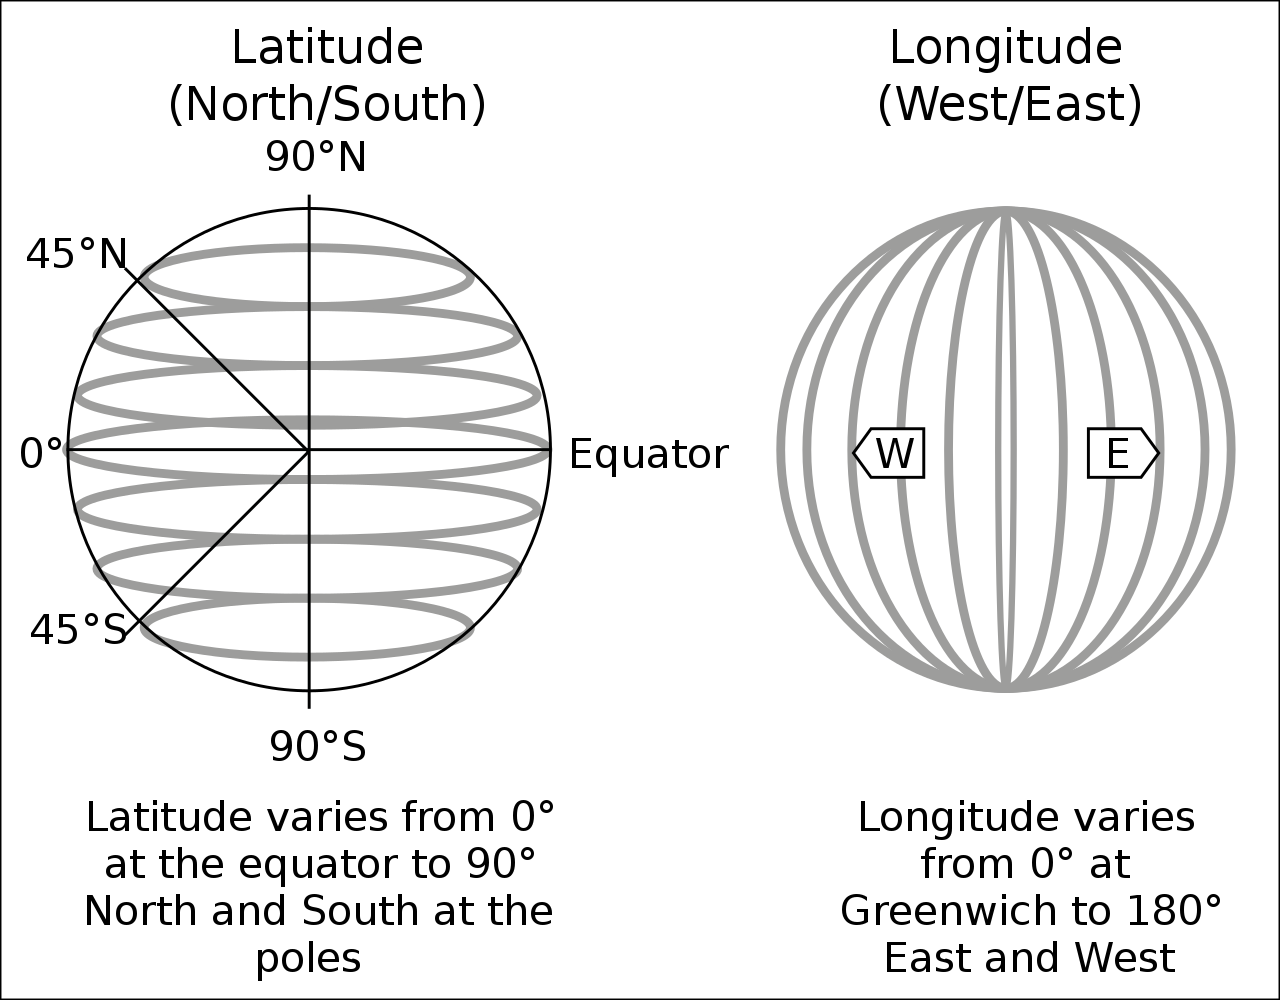
\includegraphics{fig/lat-long.png}

}

\caption{Figure: Latitude and longitude, Source:
\href{https://en.wikipedia.org/wiki/Geographic_coordinate_system}{Wikipedia}}

\end{figure}

However, we need to specify a reference point for latitudes and
longitudes (in the Figure above: equator and Greenwich). For instance,
the pair of coordinates above comes from Google Maps which returns GPS
coordinates in `WGS 84' (\href{https://epsg.io/4326}{EPSG:4326}).

\begin{Shaded}
\begin{Highlighting}[]
\CommentTok{\# Coordinate pairs of two locations}
\NormalTok{coords1 }\OtherTok{\textless{}{-}} \FunctionTok{c}\NormalTok{(}\FloatTok{51.752595}\NormalTok{, }\SpecialCharTok{{-}}\FloatTok{1.262801}\NormalTok{)}
\NormalTok{coords2 }\OtherTok{\textless{}{-}} \FunctionTok{c}\NormalTok{(}\FloatTok{51.753237}\NormalTok{, }\SpecialCharTok{{-}}\FloatTok{1.253904}\NormalTok{)}
\NormalTok{coords }\OtherTok{\textless{}{-}} \FunctionTok{rbind}\NormalTok{(coords1, coords2)}

\CommentTok{\# Conventional data frame}
\NormalTok{nuffield.df }\OtherTok{\textless{}{-}} \FunctionTok{data.frame}\NormalTok{(}\AttributeTok{name =} \FunctionTok{c}\NormalTok{(}\StringTok{"Nuffield College"}\NormalTok{, }\StringTok{"Radcliffe Camera"}\NormalTok{),}
                          \AttributeTok{address =} \FunctionTok{c}\NormalTok{(}\StringTok{"New Road"}\NormalTok{, }\StringTok{"Radcliffe Sq"}\NormalTok{),}
                          \AttributeTok{lat =}\NormalTok{ coords[,}\DecValTok{1}\NormalTok{], }\AttributeTok{lon =}\NormalTok{ coords[,}\DecValTok{2}\NormalTok{])}

\FunctionTok{head}\NormalTok{(nuffield.df)}
\end{Highlighting}
\end{Shaded}

\begin{verbatim}
                    name      address      lat       lon
coords1 Nuffield College     New Road 51.75259 -1.262801
coords2 Radcliffe Camera Radcliffe Sq 51.75324 -1.253904
\end{verbatim}

\begin{Shaded}
\begin{Highlighting}[]
\CommentTok{\# Combine to spatial data frame}
\NormalTok{nuffield.spdf }\OtherTok{\textless{}{-}} \FunctionTok{st\_as\_sf}\NormalTok{(nuffield.df, }
                          \AttributeTok{coords =} \FunctionTok{c}\NormalTok{(}\StringTok{"lon"}\NormalTok{, }\StringTok{"lat"}\NormalTok{), }\CommentTok{\# Order is important}
                          \AttributeTok{crs =} \DecValTok{4326}\NormalTok{) }\CommentTok{\# EPSG number of CRS}

\CommentTok{\# Map}
\FunctionTok{mapview}\NormalTok{(nuffield.spdf, }\AttributeTok{zcol =} \StringTok{"name"}\NormalTok{)}
\end{Highlighting}
\end{Shaded}

\begin{figure}[H]

{\centering 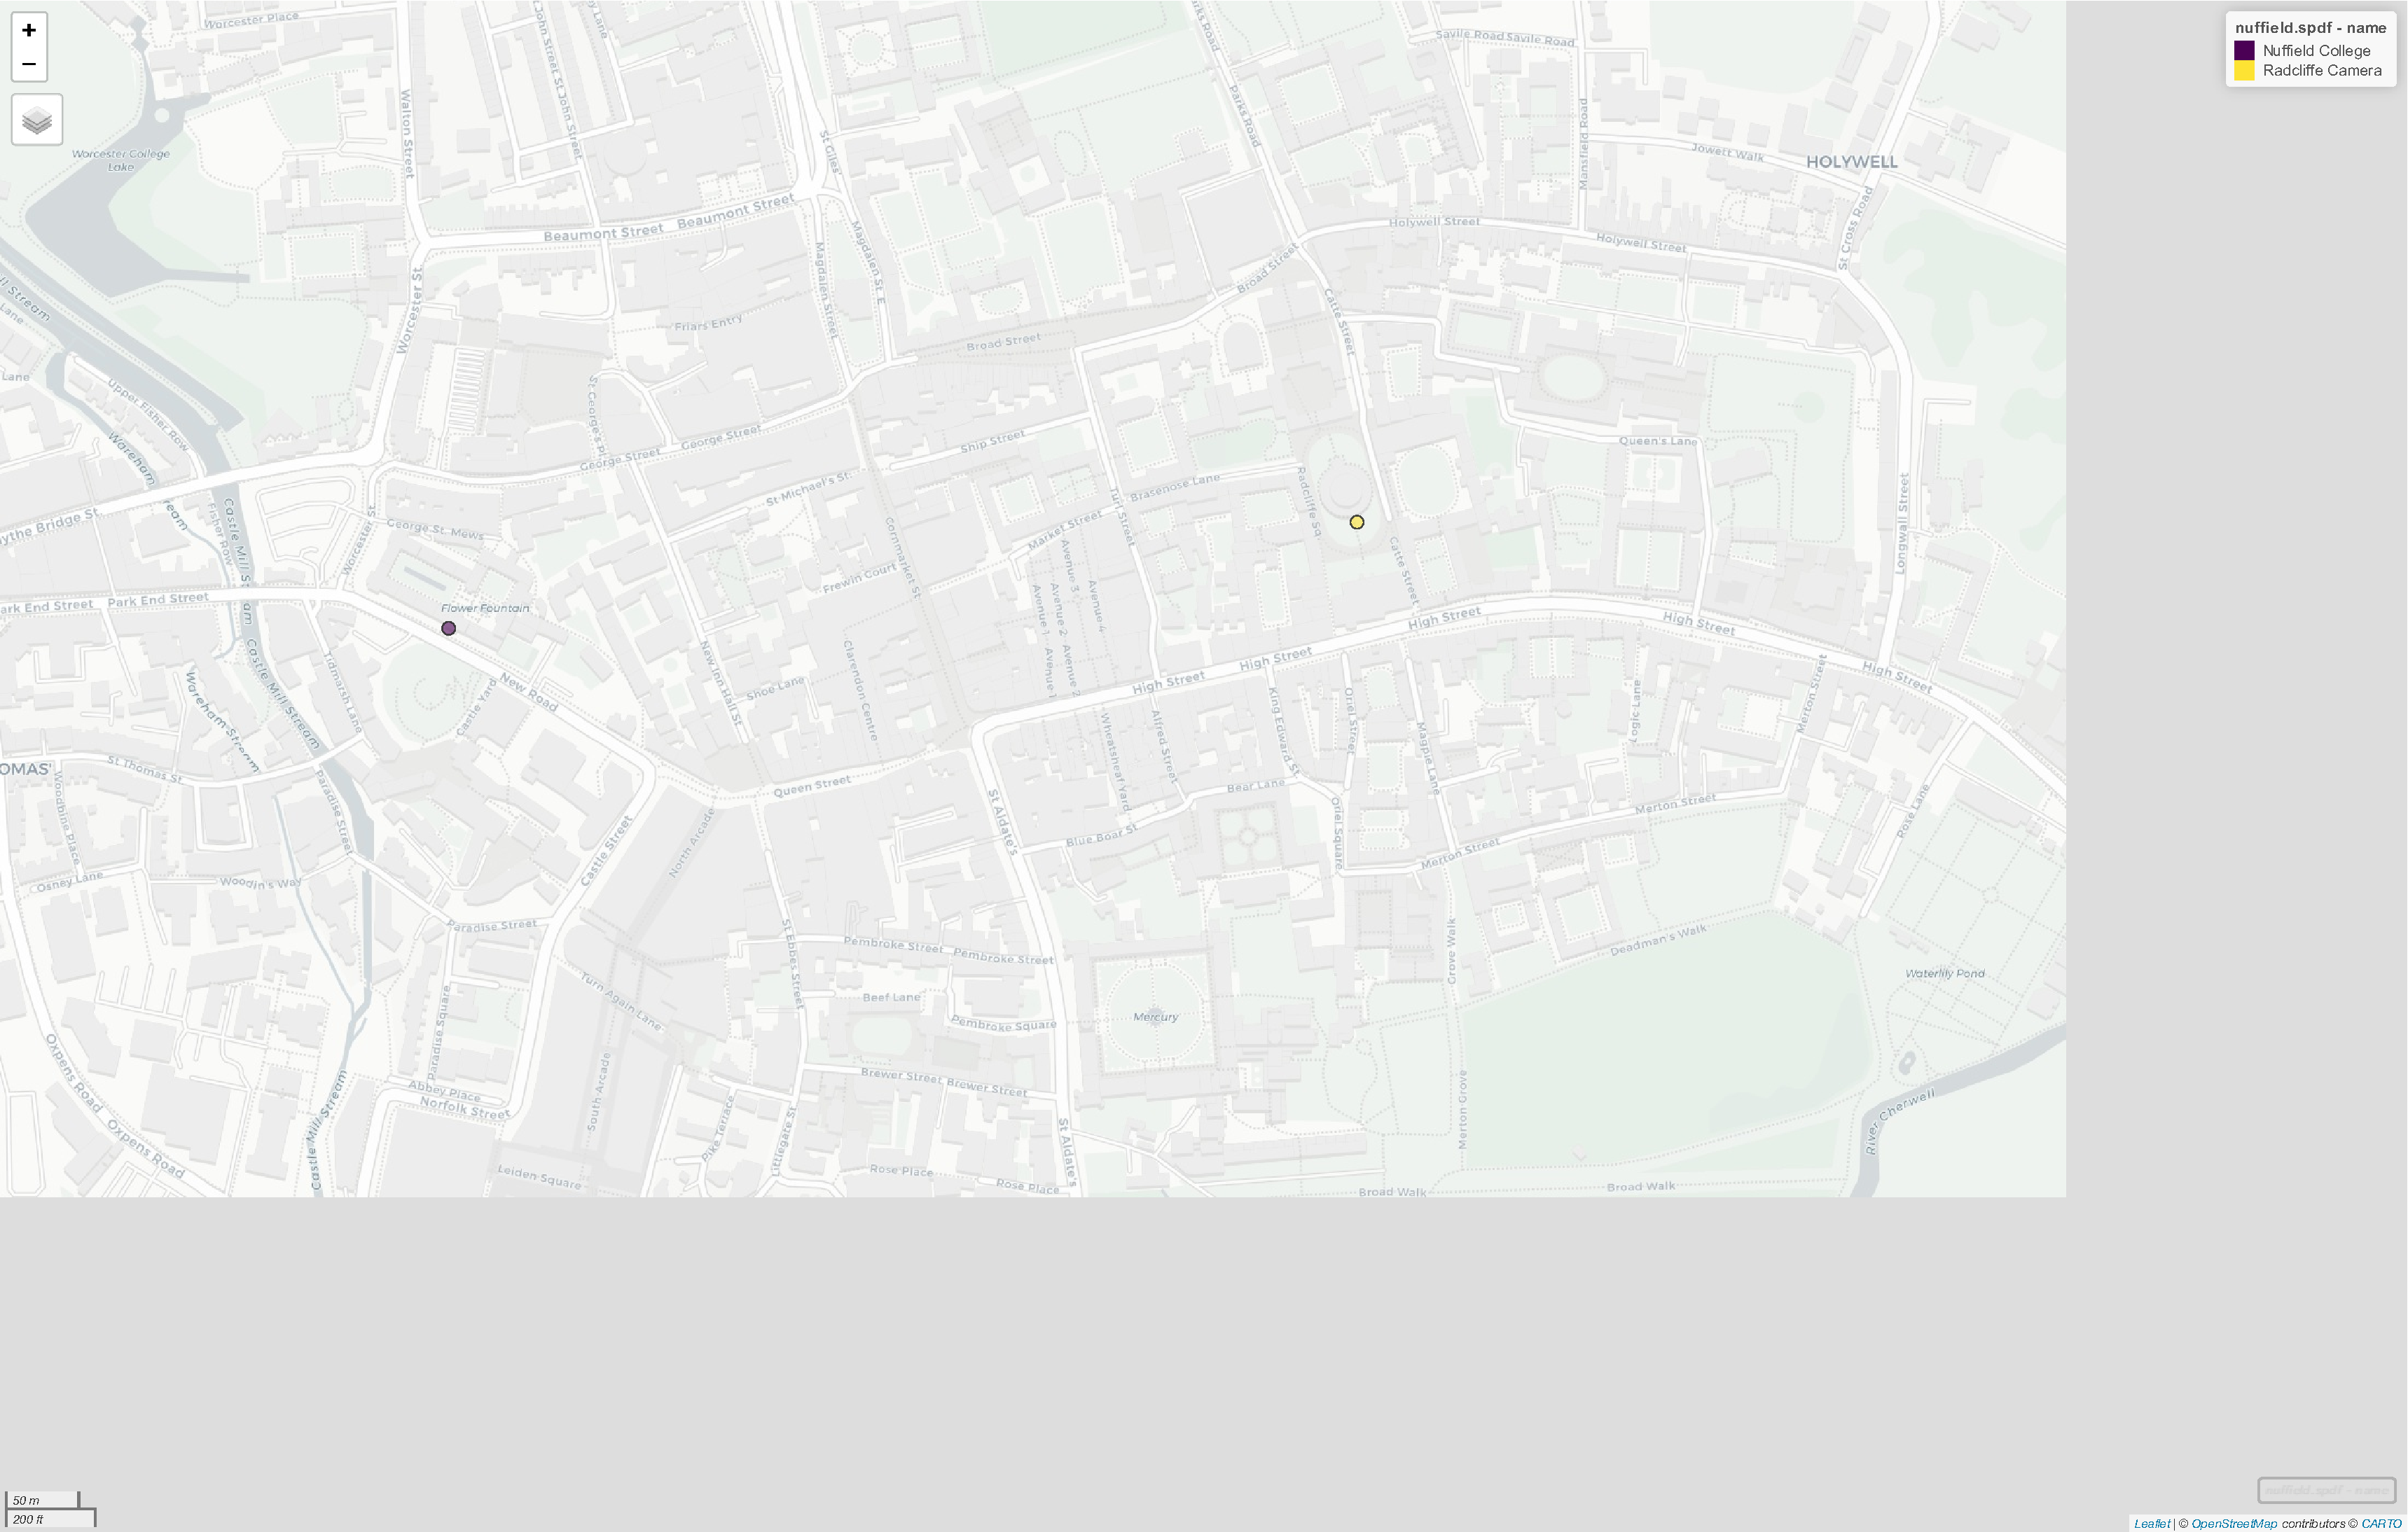
\includegraphics{01_refresher_short_files/figure-pdf/unnamed-chunk-4-1.pdf}

}

\end{figure}

\hypertarget{projected-crs}{%
\subsection{Projected CRS}\label{projected-crs}}

However, different data providers use different CRS. For instance,
spatial data in the UK usually uses `OSGB 1936 / British National Grid'
(\href{https://epsg.io/27700}{EPSG:27700}). Here, coordinates are in
meters, and projected onto a planar 2D space.

There are a lot of different CRS projections, and different national
statistics offices provide data in different projections. Data providers
usually specify which reference system they use. This is important as
using the correct reference system and projection is crucial for
plotting and manipulating spatial data.

If you do not know the correct CRS, try starting with a standards CRS
like \href{https://epsg.io/4326}{EPSG:4326} if you have decimal degree
like coordinates. If it looks like projected coordinates, try searching
for the country or region in CRS libraries like \url{https://epsg.io/}.
However, you must check if the projected coordinates match their real
location, e.g.~using \texttt{mapview()}.

\hypertarget{why-different-projections}{%
\subsection{Why different
projections?}\label{why-different-projections}}

By now, (most) people agree that
\href{https://r-spatial.org/r/2020/06/17/s2.html}{the earth is not
flat}. So, to plot data on a 2D planar surface and to perform certain
operations on a planar world, we need to make some re-projections.
Depending on where we are, different re-projections of our data (globe
in this case) might work better than others.

\begin{Shaded}
\begin{Highlighting}[]
\NormalTok{world }\OtherTok{\textless{}{-}} \FunctionTok{ne\_countries}\NormalTok{(}\AttributeTok{scale =} \StringTok{"medium"}\NormalTok{, }\AttributeTok{returnclass =} \StringTok{"sf"}\NormalTok{)}
\FunctionTok{class}\NormalTok{(world)}
\end{Highlighting}
\end{Shaded}

\begin{verbatim}
[1] "sf"         "data.frame"
\end{verbatim}

\begin{Shaded}
\begin{Highlighting}[]
\FunctionTok{st\_crs}\NormalTok{(world)}
\end{Highlighting}
\end{Shaded}

\begin{verbatim}
Coordinate Reference System:
  User input: +proj=longlat +datum=WGS84 +no_defs +ellps=WGS84 +towgs84=0,0,0 
  wkt:
BOUNDCRS[
    SOURCECRS[
        GEOGCRS["unknown",
            DATUM["World Geodetic System 1984",
                ELLIPSOID["WGS 84",6378137,298.257223563,
                    LENGTHUNIT["metre",1]],
                ID["EPSG",6326]],
            PRIMEM["Greenwich",0,
                ANGLEUNIT["degree",0.0174532925199433],
                ID["EPSG",8901]],
            CS[ellipsoidal,2],
                AXIS["longitude",east,
                    ORDER[1],
                    ANGLEUNIT["degree",0.0174532925199433,
                        ID["EPSG",9122]]],
                AXIS["latitude",north,
                    ORDER[2],
                    ANGLEUNIT["degree",0.0174532925199433,
                        ID["EPSG",9122]]]]],
    TARGETCRS[
        GEOGCRS["WGS 84",
            DATUM["World Geodetic System 1984",
                ELLIPSOID["WGS 84",6378137,298.257223563,
                    LENGTHUNIT["metre",1]]],
            PRIMEM["Greenwich",0,
                ANGLEUNIT["degree",0.0174532925199433]],
            CS[ellipsoidal,2],
                AXIS["latitude",north,
                    ORDER[1],
                    ANGLEUNIT["degree",0.0174532925199433]],
                AXIS["longitude",east,
                    ORDER[2],
                    ANGLEUNIT["degree",0.0174532925199433]],
            ID["EPSG",4326]]],
    ABRIDGEDTRANSFORMATION["Transformation from unknown to WGS84",
        METHOD["Geocentric translations (geog2D domain)",
            ID["EPSG",9603]],
        PARAMETER["X-axis translation",0,
            ID["EPSG",8605]],
        PARAMETER["Y-axis translation",0,
            ID["EPSG",8606]],
        PARAMETER["Z-axis translation",0,
            ID["EPSG",8607]]]]
\end{verbatim}

\begin{Shaded}
\begin{Highlighting}[]
\CommentTok{\# Extract a country and plot in current CRS (WGS84)}
\NormalTok{ger.spdf }\OtherTok{\textless{}{-}}\NormalTok{ world[world}\SpecialCharTok{$}\NormalTok{name }\SpecialCharTok{==} \StringTok{"Germany"}\NormalTok{, ]}
\FunctionTok{plot}\NormalTok{(}\FunctionTok{st\_geometry}\NormalTok{(ger.spdf))}
\end{Highlighting}
\end{Shaded}

\begin{figure}[H]

{\centering 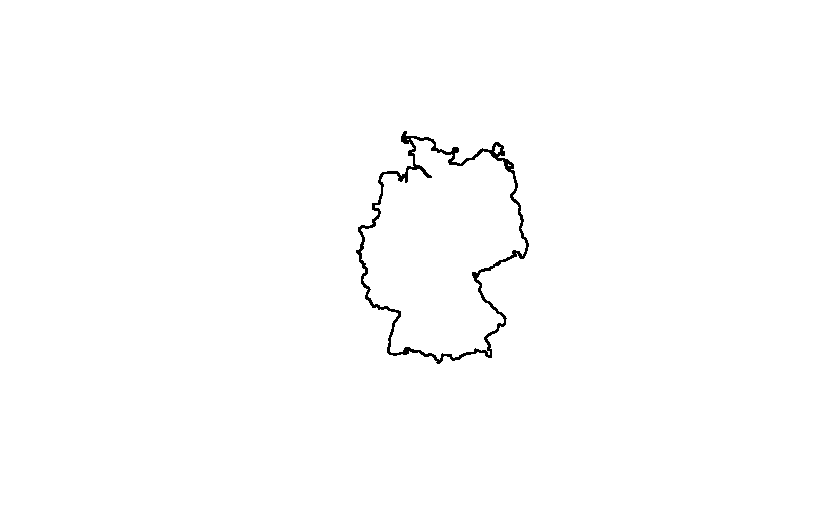
\includegraphics{01_refresher_short_files/figure-pdf/unnamed-chunk-5-1.pdf}

}

\end{figure}

\begin{Shaded}
\begin{Highlighting}[]
\CommentTok{\# Now, let\textquotesingle{}s transform Germany into a CRS optimized for Iceland}
\NormalTok{ger\_rep.spdf }\OtherTok{\textless{}{-}} \FunctionTok{st\_transform}\NormalTok{(ger.spdf, }\AttributeTok{crs =} \DecValTok{5325}\NormalTok{)}
\FunctionTok{plot}\NormalTok{(}\FunctionTok{st\_geometry}\NormalTok{(ger\_rep.spdf))}
\end{Highlighting}
\end{Shaded}

\begin{figure}[H]

{\centering 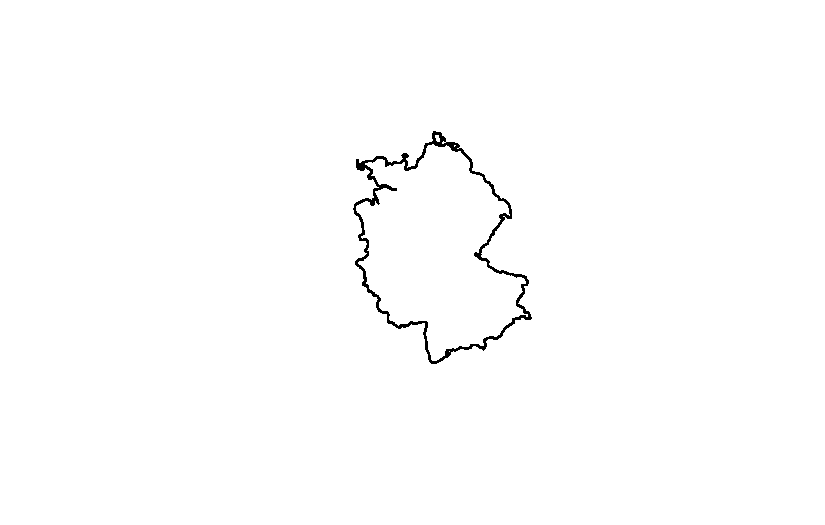
\includegraphics{01_refresher_short_files/figure-pdf/unnamed-chunk-5-2.pdf}

}

\end{figure}

Depending on the angle, a 2D projection of the earth looks different. It
is important to choose a suitable projection for the available spatial
data. For more information on CRS and re-projection, see e.g. Lovelace,
Nowosad, and Muenchow (2019) or
\href{https://stefanjuenger.github.io/}{Stefan Jünger} \&
\href{https://www.gesis.org/institut/mitarbeitendenverzeichnis/person/Anne-Kathrin.Stroppe}{Anne-Kathrin
Stroppe}'s
\href{https://github.com/StefanJuenger/gesis-workshop-geospatial-techniques-R-2023}{GESIS
workshop materials}.

\hypertarget{importing-some-real-world-data}{%
\section{Importing some real world
data}\label{importing-some-real-world-data}}

\texttt{sf} imports many of the most common spatial data files, like
geojson, gpkg, or shp.

\hypertarget{london-shapefile-polygon}{%
\subsection{London shapefile (polygon)}\label{london-shapefile-polygon}}

Let's get some administrative boundaries for London from the
\href{https://data.london.gov.uk/dataset/statistical-gis-boundary-files-london}{London
Datastore}. We use the \texttt{sf} package and its funtion
\texttt{st\_read()} to import the data.

\begin{Shaded}
\begin{Highlighting}[]
\CommentTok{\# Create subdir (all data withh be stored in "\_data")}
\NormalTok{dn }\OtherTok{\textless{}{-}} \StringTok{"\_data"}
\FunctionTok{ifelse}\NormalTok{(}\FunctionTok{dir.exists}\NormalTok{(dn), }\StringTok{"Exists"}\NormalTok{, }\FunctionTok{dir.create}\NormalTok{(dn))}
\end{Highlighting}
\end{Shaded}

\begin{verbatim}
[1] "Exists"
\end{verbatim}

\begin{Shaded}
\begin{Highlighting}[]
\CommentTok{\# Download zip file and unzip}
\NormalTok{tmpf }\OtherTok{\textless{}{-}} \FunctionTok{tempfile}\NormalTok{()}
\NormalTok{boundary.link }\OtherTok{\textless{}{-}} \StringTok{"https://data.london.gov.uk/download/statistical{-}gis{-}boundary{-}files{-}london/9ba8c833{-}6370{-}4b11{-}abdc{-}314aa020d5e0/statistical{-}gis{-}boundaries{-}london.zip"}
\FunctionTok{download.file}\NormalTok{(boundary.link, tmpf)}
\FunctionTok{unzip}\NormalTok{(}\AttributeTok{zipfile =}\NormalTok{ tmpf, }\AttributeTok{exdir =} \FunctionTok{paste0}\NormalTok{(dn))}
\FunctionTok{unlink}\NormalTok{(tmpf)}

\CommentTok{\# This is a shapefile}
\CommentTok{\# We only need the MSOA layer for now}
\NormalTok{msoa.spdf }\OtherTok{\textless{}{-}} \FunctionTok{st\_read}\NormalTok{(}\AttributeTok{dsn =} \FunctionTok{paste0}\NormalTok{(dn, }\StringTok{"/statistical{-}gis{-}boundaries{-}london/ESRI"}\NormalTok{),}
                     \AttributeTok{layer =} \StringTok{"MSOA\_2011\_London\_gen\_MHW"} \CommentTok{\# Note: no file ending}
\NormalTok{                     )}
\end{Highlighting}
\end{Shaded}

\begin{verbatim}
Reading layer `MSOA_2011_London_gen_MHW' from data source 
  `C:\work\Lehre\Geodata_Spatial_Regression_short\_data\statistical-gis-boundaries-london\ESRI' 
  using driver `ESRI Shapefile'
Simple feature collection with 983 features and 12 fields
Geometry type: MULTIPOLYGON
Dimension:     XY
Bounding box:  xmin: 503574.2 ymin: 155850.8 xmax: 561956.7 ymax: 200933.6
Projected CRS: OSGB36 / British National Grid
\end{verbatim}

The object \texttt{msoa.spdf} is our spatial data.frame. It looks
essentially like a conventional data.frame, but has some additional
attributes and geo-graphical information stored with it. Most
importantly, notice the column \texttt{geometry}, which contains a list
of polygons. In most cases, we have one polygon for each line /
observation.

\begin{Shaded}
\begin{Highlighting}[]
\FunctionTok{head}\NormalTok{(msoa.spdf)}
\end{Highlighting}
\end{Shaded}

\begin{verbatim}
Simple feature collection with 6 features and 12 fields
Geometry type: MULTIPOLYGON
Dimension:     XY
Bounding box:  xmin: 530966.7 ymin: 180510.7 xmax: 551943.8 ymax: 191139
Projected CRS: OSGB36 / British National Grid
   MSOA11CD                 MSOA11NM   LAD11CD              LAD11NM   RGN11CD
1 E02000001       City of London 001 E09000001       City of London E12000007
2 E02000002 Barking and Dagenham 001 E09000002 Barking and Dagenham E12000007
3 E02000003 Barking and Dagenham 002 E09000002 Barking and Dagenham E12000007
4 E02000004 Barking and Dagenham 003 E09000002 Barking and Dagenham E12000007
5 E02000005 Barking and Dagenham 004 E09000002 Barking and Dagenham E12000007
6 E02000007 Barking and Dagenham 006 E09000002 Barking and Dagenham E12000007
  RGN11NM USUALRES HHOLDRES COMESTRES POPDEN HHOLDS AVHHOLDSZ
1  London     7375     7187       188   25.5   4385       1.6
2  London     6775     6724        51   31.3   2713       2.5
3  London    10045    10033        12   46.9   3834       2.6
4  London     6182     5937       245   24.8   2318       2.6
5  London     8562     8562         0   72.1   3183       2.7
6  London     8791     8672       119   50.6   3441       2.5
                        geometry
1 MULTIPOLYGON (((531667.6 18...
2 MULTIPOLYGON (((548881.6 19...
3 MULTIPOLYGON (((549102.4 18...
4 MULTIPOLYGON (((551550 1873...
5 MULTIPOLYGON (((549099.6 18...
6 MULTIPOLYGON (((549819.9 18...
\end{verbatim}

Shapefiles are still among the most common formats to store and transmit
spatial data, despite them being inefficient (file size and file
number).

However, \texttt{sf} reads everything spatial, such as
\texttt{geo.json}, which usually is more efficient, but less common (but
we're getting there).

\begin{Shaded}
\begin{Highlighting}[]
\CommentTok{\# Download file}
\NormalTok{ulez.link }\OtherTok{\textless{}{-}} \StringTok{"https://data.london.gov.uk/download/ultra\_low\_emissions\_zone/936d71d8{-}c5fc{-}40ad{-}a392{-}6bec86413b48/CentralUltraLowEmissionZone.geojson"}
\FunctionTok{download.file}\NormalTok{(ulez.link, }\FunctionTok{paste0}\NormalTok{(dn, }\StringTok{"/ulez.json"}\NormalTok{))}

\CommentTok{\# Read geo.json}
\FunctionTok{st\_layers}\NormalTok{(}\FunctionTok{paste0}\NormalTok{(dn, }\StringTok{"/ulez.json"}\NormalTok{))}
\end{Highlighting}
\end{Shaded}

\begin{verbatim}
Driver: GeoJSON 
Available layers:
                   layer_name geometry_type features fields
1 CentralUltraLowEmissionZone Multi Polygon        1      4
                        crs_name
1 OSGB36 / British National Grid
\end{verbatim}

\begin{Shaded}
\begin{Highlighting}[]
\NormalTok{ulez.spdf }\OtherTok{\textless{}{-}} \FunctionTok{st\_read}\NormalTok{(}\AttributeTok{dsn =} \FunctionTok{paste0}\NormalTok{(dn, }\StringTok{"/ulez.json"}\NormalTok{)) }\CommentTok{\# here dsn is simply the file}
\end{Highlighting}
\end{Shaded}

\begin{verbatim}
Reading layer `CentralUltraLowEmissionZone' from data source 
  `C:\work\Lehre\Geodata_Spatial_Regression_short\_data\ulez.json' 
  using driver `GeoJSON'
Simple feature collection with 1 feature and 4 fields
Geometry type: MULTIPOLYGON
Dimension:     XY
Bounding box:  xmin: 527271.5 ymin: 178041.5 xmax: 533866.3 ymax: 183133.4
Projected CRS: OSGB36 / British National Grid
\end{verbatim}

\begin{Shaded}
\begin{Highlighting}[]
\FunctionTok{head}\NormalTok{(ulez.spdf)}
\end{Highlighting}
\end{Shaded}

\begin{verbatim}
Simple feature collection with 1 feature and 4 fields
Geometry type: MULTIPOLYGON
Dimension:     XY
Bounding box:  xmin: 527271.5 ymin: 178041.5 xmax: 533866.3 ymax: 183133.4
Projected CRS: OSGB36 / British National Grid
  fid OBJECTID BOUNDARY Shape_Area                       geometry
1   1        1 CSS Area   21.37557 MULTIPOLYGON (((531562.7 18...
\end{verbatim}

Again, this looks like a conventional \texttt{data.frame} but has the
additional column \texttt{geometry} containing the coordinates of each
observation. \texttt{st\_geometry()} returns only the geographic object
and \texttt{st\_drop\_geometry()} only the \texttt{data.frame} without
the coordinates. We can plot the object using \texttt{mapview()}.

\begin{Shaded}
\begin{Highlighting}[]
\FunctionTok{mapview}\NormalTok{(msoa.spdf[, }\StringTok{"POPDEN"}\NormalTok{])}
\end{Highlighting}
\end{Shaded}

\begin{figure}[H]

{\centering 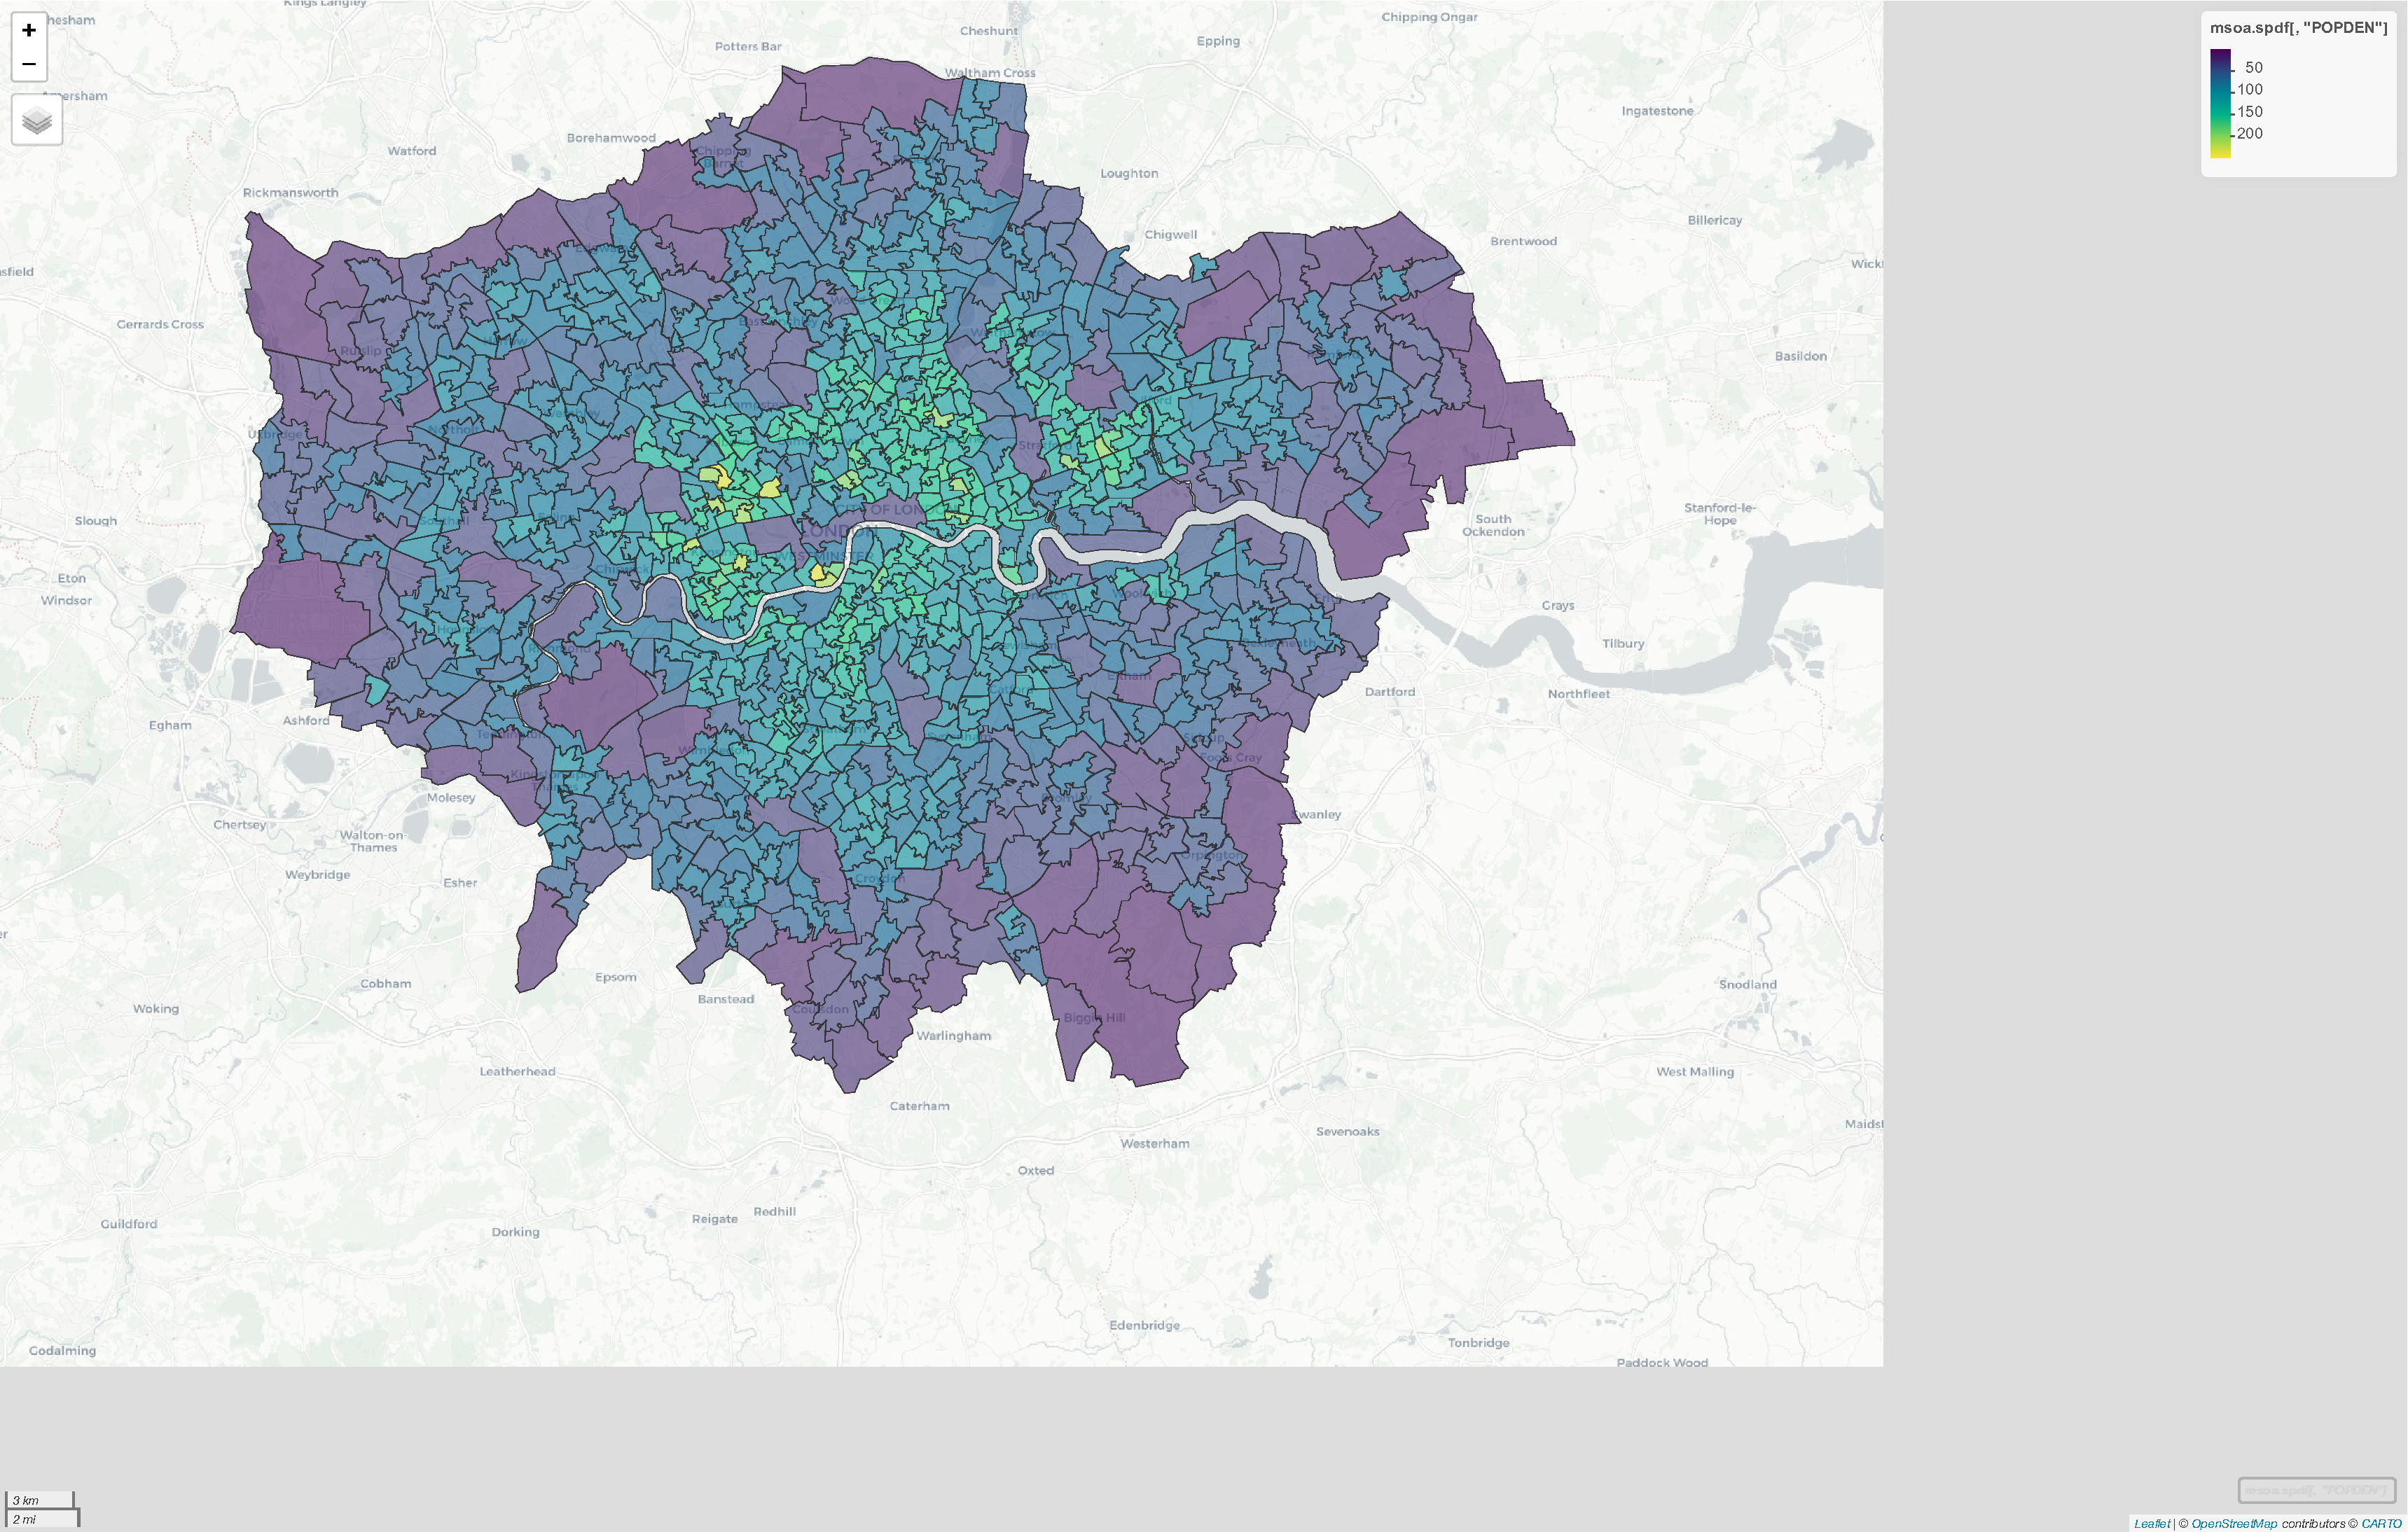
\includegraphics{01_refresher_short_files/figure-pdf/unnamed-chunk-9-1.pdf}

}

\end{figure}

\hypertarget{census-api-admin-units}{%
\subsection{Census API (admin units)}\label{census-api-admin-units}}

Now that we have some boundaries and shapes of spatial units in London,
we can start looking for different data sources to populate the
geometries.

A good source for demographic data is for instance the 2011 census.
Below we use the nomis API to retrieve population data for London, See
the
\href{https://cran.r-project.org/web/packages/nomisr/vignettes/introduction.html}{Vignette}
for more information (Guest users are limited to 25,000 rows per query).
Below is a wrapper to avoid some errors with sex and urban-rural
cross-tabulation in some of the data.

\begin{Shaded}
\begin{Highlighting}[]
\DocumentationTok{\#\#\# For larger request, register and set key}
\CommentTok{\# Sys.setenv(NOMIS\_API\_KEY = "XXX")}
\CommentTok{\# nomis\_api\_key(check\_env = TRUE)}

\NormalTok{x }\OtherTok{\textless{}{-}} \FunctionTok{nomis\_data\_info}\NormalTok{()}

\CommentTok{\# Get London ids}
\NormalTok{london\_ids }\OtherTok{\textless{}{-}}\NormalTok{ msoa.spdf}\SpecialCharTok{$}\NormalTok{MSOA11CD}

\DocumentationTok{\#\#\# Get key statistics ids}
\CommentTok{\# select requires tables (https://www.nomisweb.co.uk/sources/census\_2011\_ks)}
\CommentTok{\# Let\textquotesingle{}s get KS201EW (ethnic group), KS205EW (passport held), and KS402EW (housing tenure)}

\CommentTok{\# Get internal ids}
\NormalTok{stats }\OtherTok{\textless{}{-}} \FunctionTok{c}\NormalTok{(}\StringTok{"KS201EW"}\NormalTok{, }\StringTok{"KS402EW"}\NormalTok{, }\StringTok{"KS205EW"}\NormalTok{)}
\NormalTok{oo }\OtherTok{\textless{}{-}} \FunctionTok{which}\NormalTok{(}\FunctionTok{grepl}\NormalTok{(}\FunctionTok{paste}\NormalTok{(stats, }\AttributeTok{collapse =} \StringTok{"|"}\NormalTok{), x}\SpecialCharTok{$}\NormalTok{name.value))}
\NormalTok{ksids }\OtherTok{\textless{}{-}}\NormalTok{ x}\SpecialCharTok{$}\NormalTok{id[oo]}
\NormalTok{ksids }\CommentTok{\# This are the internal ids}
\end{Highlighting}
\end{Shaded}

\begin{verbatim}
[1] "NM_608_1" "NM_612_1" "NM_619_1"
\end{verbatim}

\begin{Shaded}
\begin{Highlighting}[]
\DocumentationTok{\#\#\# look at meta information}
\NormalTok{q }\OtherTok{\textless{}{-}} \FunctionTok{nomis\_overview}\NormalTok{(ksids[}\DecValTok{1}\NormalTok{])}
\FunctionTok{head}\NormalTok{(q)}
\end{Highlighting}
\end{Shaded}

\begin{verbatim}
# A tibble: 6 x 2
  name           value           
  <chr>          <list>          
1 analyses       <named list [1]>
2 analysisname   <chr [1]>       
3 analysisnumber <int [1]>       
4 contact        <named list [4]>
5 contenttypes   <named list [1]>
6 coverage       <chr [1]>       
\end{verbatim}

\begin{Shaded}
\begin{Highlighting}[]
\NormalTok{a }\OtherTok{\textless{}{-}} \FunctionTok{nomis\_get\_metadata}\NormalTok{(}\AttributeTok{id =}\NormalTok{ ksids[}\DecValTok{1}\NormalTok{], }\AttributeTok{concept =} \StringTok{"GEOGRAPHY"}\NormalTok{, }\AttributeTok{type =} \StringTok{"type"}\NormalTok{)}
\NormalTok{a }\CommentTok{\# TYPE297 is MSOA level}
\end{Highlighting}
\end{Shaded}

\begin{verbatim}
# A tibble: 24 x 3
   id      label.en                                           description.en    
   <chr>   <chr>                                              <chr>             
 1 TYPE265 NHS area teams                                     NHS area teams    
 2 TYPE266 clinical commissioning groups                      clinical commissi~
 3 TYPE267 built-up areas including subdivisions              built-up areas in~
 4 TYPE269 built-up areas                                     built-up areas    
 5 TYPE273 national assembly for wales electoral regions 2010 national assembly~
 6 TYPE274 postcode areas                                     postcode areas    
 7 TYPE275 postcode districts                                 postcode districts
 8 TYPE276 postcode sectors                                   postcode sectors  
 9 TYPE277 national assembly for wales constituencies 2010    national assembly~
10 TYPE279 parishes 2011                                      parishes 2011     
# i 14 more rows
\end{verbatim}

\begin{Shaded}
\begin{Highlighting}[]
\NormalTok{b }\OtherTok{\textless{}{-}} \FunctionTok{nomis\_get\_metadata}\NormalTok{(}\AttributeTok{id =}\NormalTok{ ksids[}\DecValTok{1}\NormalTok{], }\AttributeTok{concept =} \StringTok{"MEASURES"}\NormalTok{, }\AttributeTok{type =} \StringTok{"TYPE297"}\NormalTok{)}
\NormalTok{b }\CommentTok{\# 20100 is the measure of absolute numbers}
\end{Highlighting}
\end{Shaded}

\begin{verbatim}
# A tibble: 2 x 3
  id    label.en description.en
  <chr> <chr>    <chr>         
1 20100 value    value         
2 20301 percent  percent       
\end{verbatim}

\begin{Shaded}
\begin{Highlighting}[]
\DocumentationTok{\#\#\# Query data in loop over the required statistics}
\ControlFlowTok{for}\NormalTok{(i }\ControlFlowTok{in}\NormalTok{ ksids)\{}

  \CommentTok{\# Determin if data is divided by sex or urban{-}rural}
\NormalTok{  nd }\OtherTok{\textless{}{-}} \FunctionTok{nomis\_get\_metadata}\NormalTok{(}\AttributeTok{id =}\NormalTok{ i)}
  \ControlFlowTok{if}\NormalTok{(}\StringTok{"RURAL\_URBAN"} \SpecialCharTok{\%in\%}\NormalTok{ nd}\SpecialCharTok{$}\NormalTok{conceptref)\{}
\NormalTok{    UR }\OtherTok{\textless{}{-}} \ConstantTok{TRUE}
\NormalTok{  \}}\ControlFlowTok{else}\NormalTok{\{}
\NormalTok{    UR }\OtherTok{\textless{}{-}} \ConstantTok{FALSE}
\NormalTok{  \}}
  \ControlFlowTok{if}\NormalTok{(}\StringTok{"C\_SEX"} \SpecialCharTok{\%in\%}\NormalTok{ nd}\SpecialCharTok{$}\NormalTok{conceptref)\{}
\NormalTok{    SEX }\OtherTok{\textless{}{-}} \ConstantTok{TRUE}
\NormalTok{  \}}\ControlFlowTok{else}\NormalTok{\{}
\NormalTok{    SEX }\OtherTok{\textless{}{-}} \ConstantTok{FALSE}
\NormalTok{  \}}

  \CommentTok{\# make data request}
  \ControlFlowTok{if}\NormalTok{(UR }\SpecialCharTok{==} \ConstantTok{TRUE}\NormalTok{)\{}
    \ControlFlowTok{if}\NormalTok{(SEX }\SpecialCharTok{==} \ConstantTok{TRUE}\NormalTok{)\{}
\NormalTok{      tmp\_en }\OtherTok{\textless{}{-}} \FunctionTok{nomis\_get\_data}\NormalTok{(}\AttributeTok{id =}\NormalTok{ i, }\AttributeTok{time =} \StringTok{"2011"}\NormalTok{,}
                               \AttributeTok{geography =}\NormalTok{ london\_ids, }\CommentTok{\# replace with "TYPE297" for all MSOAs}
                               \AttributeTok{measures =} \DecValTok{20100}\NormalTok{, }\AttributeTok{RURAL\_URBAN =} \DecValTok{0}\NormalTok{, }\AttributeTok{C\_SEX =} \DecValTok{0}\NormalTok{)}
\NormalTok{    \}}\ControlFlowTok{else}\NormalTok{\{}
\NormalTok{      tmp\_en }\OtherTok{\textless{}{-}} \FunctionTok{nomis\_get\_data}\NormalTok{(}\AttributeTok{id =}\NormalTok{ i, }\AttributeTok{time =} \StringTok{"2011"}\NormalTok{,}
                               \AttributeTok{geography =}\NormalTok{ london\_ids, }\CommentTok{\# replace with "TYPE297" for all MSOAs}
                               \AttributeTok{measures =} \DecValTok{20100}\NormalTok{, }\AttributeTok{RURAL\_URBAN =} \DecValTok{0}\NormalTok{)}
\NormalTok{    \}}
\NormalTok{  \}}\ControlFlowTok{else}\NormalTok{\{}
    \ControlFlowTok{if}\NormalTok{(SEX }\SpecialCharTok{==} \ConstantTok{TRUE}\NormalTok{)\{}
\NormalTok{      tmp\_en }\OtherTok{\textless{}{-}} \FunctionTok{nomis\_get\_data}\NormalTok{(}\AttributeTok{id =}\NormalTok{ i, }\AttributeTok{time =} \StringTok{"2011"}\NormalTok{,}
                               \AttributeTok{geography =}\NormalTok{ london\_ids, }\CommentTok{\# replace with "TYPE297" for all MSOAs}
                               \AttributeTok{measures =} \DecValTok{20100}\NormalTok{, }\AttributeTok{C\_SEX =} \DecValTok{0}\NormalTok{)}
\NormalTok{    \}}\ControlFlowTok{else}\NormalTok{\{}
\NormalTok{      tmp\_en }\OtherTok{\textless{}{-}} \FunctionTok{nomis\_get\_data}\NormalTok{(}\AttributeTok{id =}\NormalTok{ i, }\AttributeTok{time =} \StringTok{"2011"}\NormalTok{,}
                               \AttributeTok{geography =}\NormalTok{ london\_ids, }\CommentTok{\# replace with "TYPE297" for all MSOAs}
                               \AttributeTok{measures =} \DecValTok{20100}\NormalTok{)}
\NormalTok{    \}}

\NormalTok{  \}}

  \CommentTok{\# Append (in case of different regions)}
\NormalTok{  ks\_tmp }\OtherTok{\textless{}{-}}\NormalTok{ tmp\_en}

  \CommentTok{\# Make lower case names}
  \FunctionTok{names}\NormalTok{(ks\_tmp) }\OtherTok{\textless{}{-}} \FunctionTok{tolower}\NormalTok{(}\FunctionTok{names}\NormalTok{(ks\_tmp))}
  \FunctionTok{names}\NormalTok{(ks\_tmp)[}\FunctionTok{names}\NormalTok{(ks\_tmp) }\SpecialCharTok{==} \StringTok{"geography\_code"}\NormalTok{] }\OtherTok{\textless{}{-}} \StringTok{"msoa11"}
  \FunctionTok{names}\NormalTok{(ks\_tmp)[}\FunctionTok{names}\NormalTok{(ks\_tmp) }\SpecialCharTok{==} \StringTok{"geography\_name"}\NormalTok{] }\OtherTok{\textless{}{-}} \StringTok{"name"}

  \CommentTok{\# replace weird cell codes}
\NormalTok{  onlynum }\OtherTok{\textless{}{-}} \FunctionTok{which}\NormalTok{(}\FunctionTok{grepl}\NormalTok{(}\StringTok{"\^{}[[:digit:]]+$"}\NormalTok{, ks\_tmp}\SpecialCharTok{$}\NormalTok{cell\_code))}
  \ControlFlowTok{if}\NormalTok{(}\FunctionTok{length}\NormalTok{(onlynum) }\SpecialCharTok{!=} \DecValTok{0}\NormalTok{)\{}
\NormalTok{    code }\OtherTok{\textless{}{-}} \FunctionTok{substr}\NormalTok{(ks\_tmp}\SpecialCharTok{$}\NormalTok{cell\_code[}\SpecialCharTok{{-}}\NormalTok{onlynum][}\DecValTok{1}\NormalTok{], }\DecValTok{1}\NormalTok{, }\DecValTok{7}\NormalTok{)}
    \ControlFlowTok{if}\NormalTok{(}\FunctionTok{is.na}\NormalTok{(code))\{}
\NormalTok{      code }\OtherTok{\textless{}{-}}\NormalTok{ i}
\NormalTok{    \}}
\NormalTok{    ks\_tmp}\SpecialCharTok{$}\NormalTok{cell\_code[onlynum] }\OtherTok{\textless{}{-}} \FunctionTok{paste0}\NormalTok{(code, }\StringTok{"\_"}\NormalTok{, ks\_tmp}\SpecialCharTok{$}\NormalTok{cell\_code[onlynum])}
\NormalTok{  \}}

  \CommentTok{\# save codebook}
\NormalTok{  ks\_cb }\OtherTok{\textless{}{-}} \FunctionTok{unique}\NormalTok{(ks\_tmp[, }\FunctionTok{c}\NormalTok{(}\StringTok{"date"}\NormalTok{, }\StringTok{"cell\_type"}\NormalTok{, }\StringTok{"cell"}\NormalTok{, }\StringTok{"cell\_code"}\NormalTok{, }\StringTok{"cell\_name"}\NormalTok{)])}

  \DocumentationTok{\#\#\# Reshape}
\NormalTok{  ks\_res }\OtherTok{\textless{}{-}}\NormalTok{ tidyr}\SpecialCharTok{::}\FunctionTok{pivot\_wider}\NormalTok{(ks\_tmp, }\AttributeTok{id\_cols =} \FunctionTok{c}\NormalTok{(}\StringTok{"msoa11"}\NormalTok{, }\StringTok{"name"}\NormalTok{),}
                               \AttributeTok{names\_from =} \StringTok{"cell\_code"}\NormalTok{,}
                               \AttributeTok{values\_from =} \StringTok{"obs\_value"}\NormalTok{)}

  \DocumentationTok{\#\#\# Merge}
  \ControlFlowTok{if}\NormalTok{(i }\SpecialCharTok{==}\NormalTok{ ksids[}\DecValTok{1}\NormalTok{])\{}
\NormalTok{    census\_keystat.df }\OtherTok{\textless{}{-}}\NormalTok{ ks\_res}
\NormalTok{    census\_keystat\_cb.df }\OtherTok{\textless{}{-}}\NormalTok{ ks\_cb}
\NormalTok{  \}}\ControlFlowTok{else}\NormalTok{\{}
\NormalTok{    census\_keystat.df }\OtherTok{\textless{}{-}} \FunctionTok{merge}\NormalTok{(census\_keystat.df, ks\_res, }\AttributeTok{by =} \FunctionTok{c}\NormalTok{(}\StringTok{"msoa11"}\NormalTok{, }\StringTok{"name"}\NormalTok{), }\AttributeTok{all =} \ConstantTok{TRUE}\NormalTok{)}
\NormalTok{    census\_keystat\_cb.df }\OtherTok{\textless{}{-}} \FunctionTok{rbind}\NormalTok{(census\_keystat\_cb.df, ks\_cb)}
\NormalTok{  \}}

\NormalTok{\}}


\CommentTok{\# Descriptions are saved in the codebook}
\FunctionTok{head}\NormalTok{(census\_keystat\_cb.df)}
\end{Highlighting}
\end{Shaded}

\begin{verbatim}
# A tibble: 6 x 5
   date cell_type     cell cell_code   cell_name                                
  <dbl> <chr>        <dbl> <chr>       <chr>                                    
1  2011 Ethnic Group     0 KS201EW0001 All usual residents                      
2  2011 Ethnic Group   100 KS201EW_100 White                                    
3  2011 Ethnic Group     1 KS201EW0002 White: English/Welsh/Scottish/Northern I~
4  2011 Ethnic Group     2 KS201EW0003 White: Irish                             
5  2011 Ethnic Group     3 KS201EW0004 White: Gypsy or Irish Traveller          
6  2011 Ethnic Group     4 KS201EW0005 White: Other White                       
\end{verbatim}

\begin{Shaded}
\begin{Highlighting}[]
\FunctionTok{save}\NormalTok{(census\_keystat\_cb.df, }\AttributeTok{file =} \StringTok{"\_data/Census\_codebook.RData"}\NormalTok{)}
\end{Highlighting}
\end{Shaded}

Now, we have one file containing the geometries of MSOAs and one file
with the census information on ethnic groups. Obviously, we can easily
merge them together using the MSOA identifiers.

\begin{Shaded}
\begin{Highlighting}[]
\NormalTok{msoa.spdf }\OtherTok{\textless{}{-}} \FunctionTok{merge}\NormalTok{(msoa.spdf, census\_keystat.df,}
                   \AttributeTok{by.x =} \StringTok{"MSOA11CD"}\NormalTok{, }\AttributeTok{by.y =} \StringTok{"msoa11"}\NormalTok{, }\AttributeTok{all.x =} \ConstantTok{TRUE}\NormalTok{)}
\end{Highlighting}
\end{Shaded}

And we can, for instance, plot the spatial distribution of ethnic
groups.

\begin{Shaded}
\begin{Highlighting}[]
\NormalTok{msoa.spdf}\SpecialCharTok{$}\NormalTok{per\_white }\OtherTok{\textless{}{-}}\NormalTok{ msoa.spdf}\SpecialCharTok{$}\NormalTok{KS201EW\_100 }\SpecialCharTok{/}\NormalTok{ msoa.spdf}\SpecialCharTok{$}\NormalTok{KS201EW0001 }\SpecialCharTok{*} \DecValTok{100}
\NormalTok{msoa.spdf}\SpecialCharTok{$}\NormalTok{per\_mixed }\OtherTok{\textless{}{-}}\NormalTok{ msoa.spdf}\SpecialCharTok{$}\NormalTok{KS201EW\_200 }\SpecialCharTok{/}\NormalTok{ msoa.spdf}\SpecialCharTok{$}\NormalTok{KS201EW0001 }\SpecialCharTok{*} \DecValTok{100}
\NormalTok{msoa.spdf}\SpecialCharTok{$}\NormalTok{per\_asian }\OtherTok{\textless{}{-}}\NormalTok{ msoa.spdf}\SpecialCharTok{$}\NormalTok{KS201EW\_300 }\SpecialCharTok{/}\NormalTok{ msoa.spdf}\SpecialCharTok{$}\NormalTok{KS201EW0001 }\SpecialCharTok{*} \DecValTok{100}
\NormalTok{msoa.spdf}\SpecialCharTok{$}\NormalTok{per\_black }\OtherTok{\textless{}{-}}\NormalTok{ msoa.spdf}\SpecialCharTok{$}\NormalTok{KS201EW\_400 }\SpecialCharTok{/}\NormalTok{ msoa.spdf}\SpecialCharTok{$}\NormalTok{KS201EW0001 }\SpecialCharTok{*} \DecValTok{100}
\NormalTok{msoa.spdf}\SpecialCharTok{$}\NormalTok{per\_other }\OtherTok{\textless{}{-}}\NormalTok{ msoa.spdf}\SpecialCharTok{$}\NormalTok{KS201EW\_500 }\SpecialCharTok{/}\NormalTok{ msoa.spdf}\SpecialCharTok{$}\NormalTok{KS201EW0001 }\SpecialCharTok{*} \DecValTok{100}

\FunctionTok{mapview}\NormalTok{(msoa.spdf[, }\StringTok{"per\_white"}\NormalTok{])}
\end{Highlighting}
\end{Shaded}

\begin{figure}[H]

{\centering 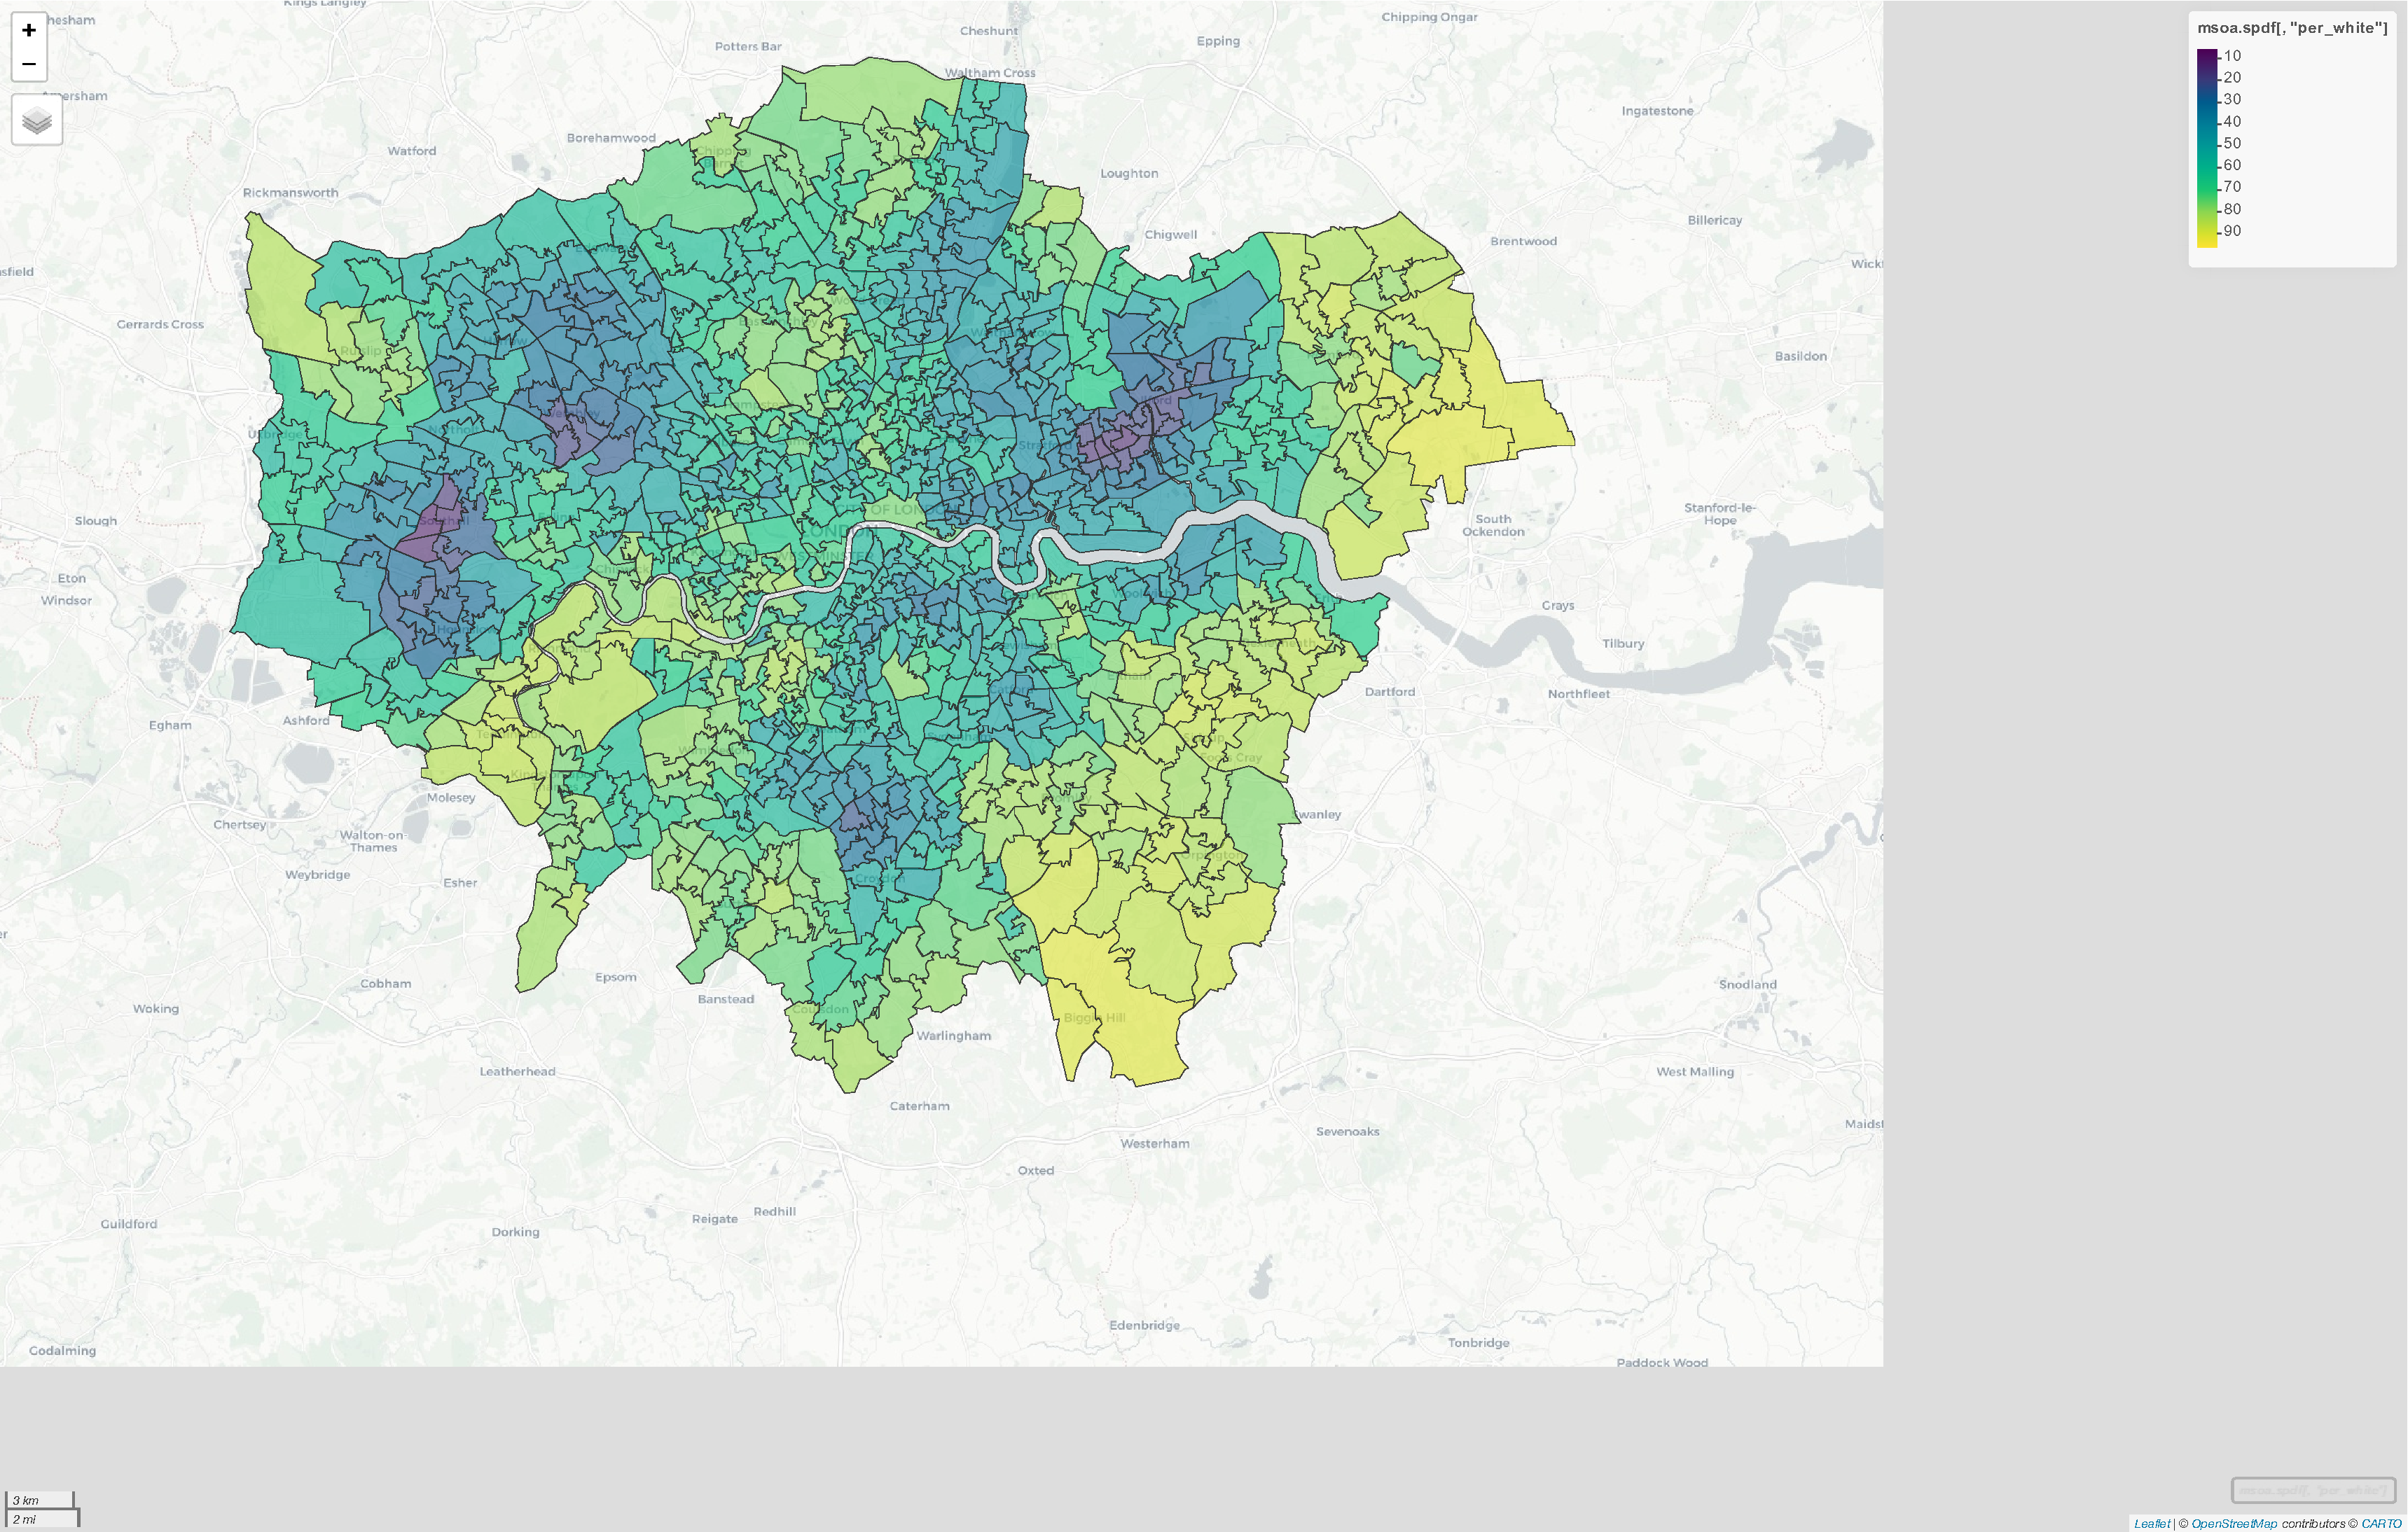
\includegraphics{01_refresher_short_files/figure-pdf/unnamed-chunk-12-1.pdf}

}

\end{figure}

If you're interested in more data sources, see for instance
\href{https://bookdown.org/paul/apis_for_social_scientists/}{APIs for
social scientists: A collaborative review} by Paul C. Bauer, Camille
Landesvatter, Lion Behrens. It's a collection of several APIs for social
sciences.

\hypertarget{gridded-data}{%
\subsection{Gridded data}\label{gridded-data}}

So far, we have queried data on administrative units. However, often
data comes on other spatial scales. For instance, we might be interested
in the amount of air pollution, which is provided on a regular grid
across the UK from
\href{https://uk-air.defra.gov.uk/data/pcm-data}{Defra}.

\begin{Shaded}
\begin{Highlighting}[]
\CommentTok{\# Download}
\NormalTok{pol.link }\OtherTok{\textless{}{-}} \StringTok{"https://uk{-}air.defra.gov.uk/datastore/pcm/mapno22011.csv"}
\FunctionTok{download.file}\NormalTok{(pol.link, }\FunctionTok{paste0}\NormalTok{(dn, }\StringTok{"/mapno22011.csv"}\NormalTok{))}
\NormalTok{pol.df }\OtherTok{\textless{}{-}} \FunctionTok{read.csv}\NormalTok{(}\FunctionTok{paste0}\NormalTok{(dn, }\StringTok{"/mapno22011.csv"}\NormalTok{), }\AttributeTok{skip =} \DecValTok{5}\NormalTok{, }\AttributeTok{header =}\NormalTok{ T, }\AttributeTok{sep =} \StringTok{","}\NormalTok{,}
                      \AttributeTok{stringsAsFactors =}\NormalTok{ F, }\AttributeTok{na.strings =} \StringTok{"MISSING"}\NormalTok{)}

\FunctionTok{head}\NormalTok{(pol.df)}
\end{Highlighting}
\end{Shaded}

\begin{verbatim}
  ukgridcode      x       y no22011
1      54291 460500 1221500      NA
2      54292 461500 1221500      NA
3      54294 463500 1221500      NA
4      54979 458500 1220500      NA
5      54980 459500 1220500      NA
6      54981 460500 1220500      NA
\end{verbatim}

The data comes as point data with x and y as coordinates. We have to
transform this into spatial data first. We first setup a spatial points
object with \texttt{st\_as\_sf}. Subsequently, we transform the point
coordinates into a regular grid. We use a buffer method
\texttt{st\_buffer} with ``diameter'', and only one segment per quadrant
(\texttt{nQuadSegs}). This gives us a 1x1km regular grid.

\begin{Shaded}
\begin{Highlighting}[]
\CommentTok{\# Build spatial object}
\NormalTok{pol.spdf }\OtherTok{\textless{}{-}} \FunctionTok{st\_as\_sf}\NormalTok{(pol.df, }\AttributeTok{coords =} \FunctionTok{c}\NormalTok{(}\StringTok{"x"}\NormalTok{, }\StringTok{"y"}\NormalTok{),}
                    \AttributeTok{crs =} \DecValTok{27700}\NormalTok{)}

\CommentTok{\# we transform the point coordinates into a regular grid with "diameter" 500m}
\NormalTok{pol.spdf }\OtherTok{\textless{}{-}} \FunctionTok{st\_buffer}\NormalTok{(pol.spdf, }\AttributeTok{dist =} \DecValTok{500}\NormalTok{, }\AttributeTok{nQuadSegs  =} \DecValTok{1}\NormalTok{,}
                      \AttributeTok{endCapStyle =} \StringTok{\textquotesingle{}SQUARE\textquotesingle{}}\NormalTok{)}

\CommentTok{\# Plot NO2}
\FunctionTok{plot}\NormalTok{(pol.spdf[, }\StringTok{"no22011"}\NormalTok{], }\AttributeTok{border =} \ConstantTok{NA}\NormalTok{)}
\end{Highlighting}
\end{Shaded}

\begin{figure}[H]

{\centering 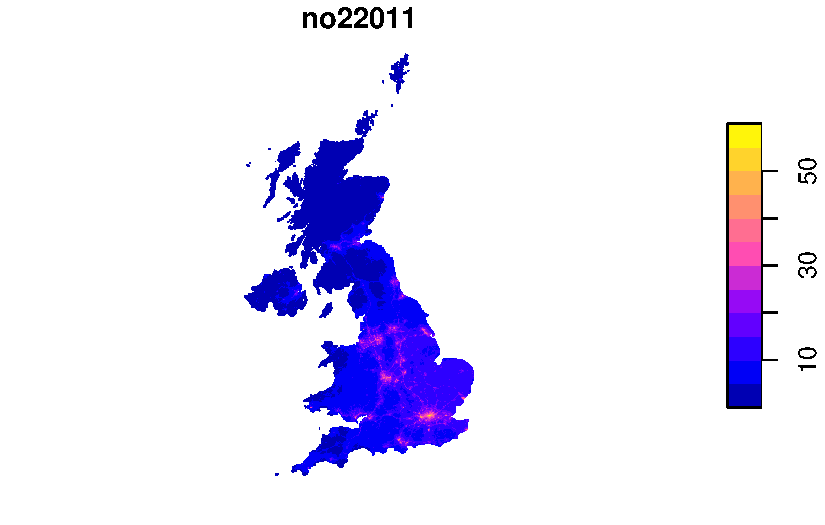
\includegraphics{01_refresher_short_files/figure-pdf/unnamed-chunk-14-1.pdf}

}

\end{figure}

\hypertarget{openstreetmap-points}{%
\subsection{OpenStreetMap (points)}\label{openstreetmap-points}}

Another interesting data source is the OpenStreetMap API, which provides
information about the geographical location of a serious of different
indicators. Robin Lovelace provides a nice introduction to the
\href{https://cran.r-project.org/web/packages/osmdata/vignettes/osmdata.html}{osmdata
API}. Available features can be found on
\href{https://wiki.openstreetmap.org/wiki/Map_features}{OSM wiki}.

First we create a bounding box of where we want to query data.
\texttt{st\_bbox()} can be used to get bounding boxes of an existing
spatial object (needs \texttt{CRS\ =\ 4326}). An alternative would be to
use
\texttt{opq(bbox\ =\ \textquotesingle{}greater\ london\ uk\textquotesingle{})}.

\begin{Shaded}
\begin{Highlighting}[]
\CommentTok{\# bounding box of where we want to query data}
\NormalTok{q }\OtherTok{\textless{}{-}} \FunctionTok{opq}\NormalTok{(}\AttributeTok{bbox =} \FunctionTok{st\_bbox}\NormalTok{(}\FunctionTok{st\_transform}\NormalTok{(msoa.spdf, }\DecValTok{4326}\NormalTok{)))}
\end{Highlighting}
\end{Shaded}

And we want to get data for all pubs and bars which are within this
bounding box.

\begin{Shaded}
\begin{Highlighting}[]
\CommentTok{\# First build the query of location of pubs in London}
\NormalTok{osmq }\OtherTok{\textless{}{-}} \FunctionTok{add\_osm\_feature}\NormalTok{(q, }\AttributeTok{key =} \StringTok{"amenity"}\NormalTok{, }\AttributeTok{value =} \StringTok{"pub"}\NormalTok{)}

\CommentTok{\# And then query the data}
\NormalTok{pubs.osm }\OtherTok{\textless{}{-}} \FunctionTok{osmdata\_sf}\NormalTok{(osmq)}
\end{Highlighting}
\end{Shaded}

Right now there are some results in polygons, some in points, and they
overlap. Often, data from OSM needs some manual cleaning. Sometimes the
same features are represented by different spatial objects (e.g.~points
+ polygons).

\begin{Shaded}
\begin{Highlighting}[]
\CommentTok{\# Make unique points / polygons}
\NormalTok{pubs.osm }\OtherTok{\textless{}{-}} \FunctionTok{unique\_osmdata}\NormalTok{(pubs.osm)}

\CommentTok{\# Get points and polygons (there are barley any pubs as polygons, so we ignore them)}
\NormalTok{pubs.points }\OtherTok{\textless{}{-}}\NormalTok{ pubs.osm}\SpecialCharTok{$}\NormalTok{osm\_points}
\NormalTok{pubs.polys }\OtherTok{\textless{}{-}}\NormalTok{ pubs.osm}\SpecialCharTok{$}\NormalTok{osm\_multipolygons}

\CommentTok{\# \# Drop OSM file}
\CommentTok{\# rm(pubs.osm); gc()}

\CommentTok{\# Reduce to point object only}
\NormalTok{pubs.spdf }\OtherTok{\textless{}{-}}\NormalTok{ pubs.points}

\CommentTok{\# Reduce to a few variables}
\NormalTok{pubs.spdf }\OtherTok{\textless{}{-}}\NormalTok{ pubs.spdf[, }\FunctionTok{c}\NormalTok{(}\StringTok{"osm\_id"}\NormalTok{, }\StringTok{"name"}\NormalTok{, }\StringTok{"addr:postcode"}\NormalTok{, }\StringTok{"diet:vegan"}\NormalTok{)]}
\end{Highlighting}
\end{Shaded}

Again, we can inspect the results with \texttt{mapview}.

\begin{Shaded}
\begin{Highlighting}[]
\FunctionTok{mapview}\NormalTok{(}\FunctionTok{st\_geometry}\NormalTok{(pubs.spdf))}
\end{Highlighting}
\end{Shaded}

\begin{figure}[H]

{\centering 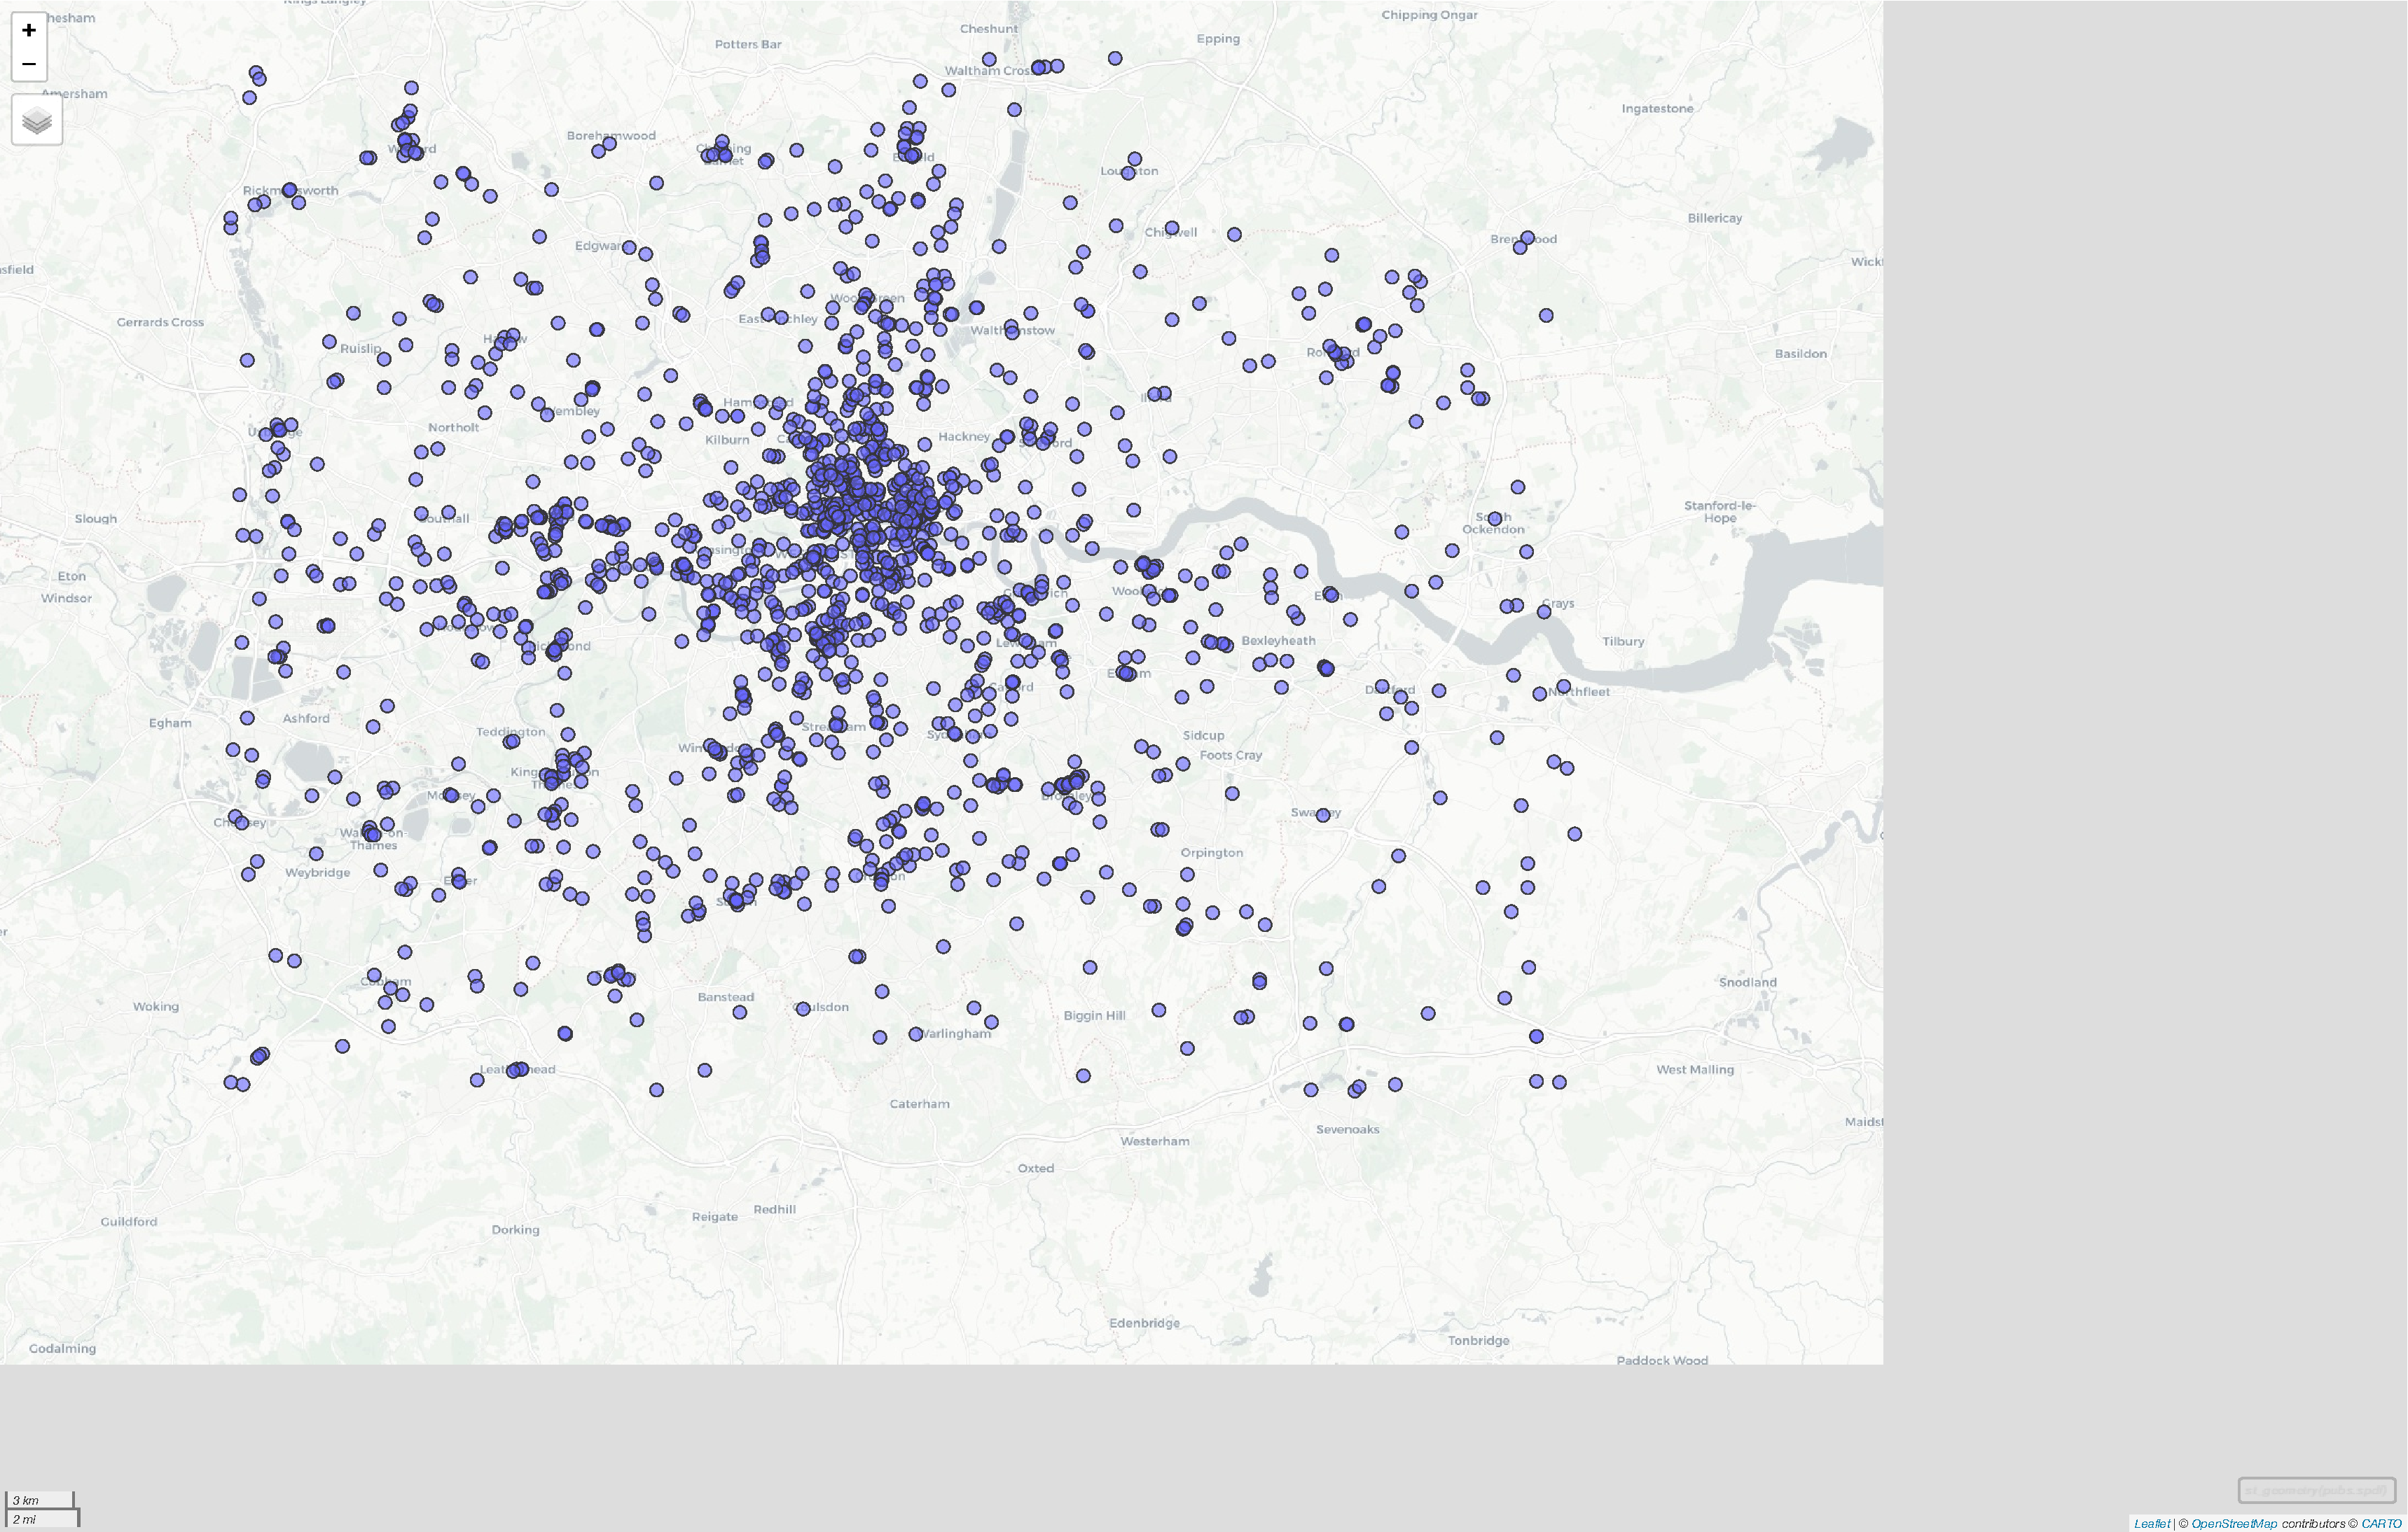
\includegraphics{01_refresher_short_files/figure-pdf/unnamed-chunk-19-1.pdf}

}

\end{figure}

Note that OSM is solely based on contribution by users, and the
\textbf{quality of OSM data varies}. Usually data quality is better in
larger cities, and better for more stable features (such as hospitals,
train stations, highways) rahter than pubs or restaurants which
regularly appear and disappear. However, data from
\href{https://data.london.gov.uk/dataset/cultural-infrastructure-map}{London
Datastore} would indicate more pubs than what we find with OSM.

\hypertarget{save}{%
\subsection{Save}\label{save}}

We will store the created data to use them again in the next session.

\begin{Shaded}
\begin{Highlighting}[]
\FunctionTok{save}\NormalTok{(msoa.spdf, }\AttributeTok{file =} \StringTok{"\_data/msoa\_spatial.RData"}\NormalTok{)}
\FunctionTok{save}\NormalTok{(ulez.spdf, }\AttributeTok{file =} \StringTok{"\_data/ulez\_spatial.RData"}\NormalTok{)}
\FunctionTok{save}\NormalTok{(pol.spdf, }\AttributeTok{file =} \StringTok{"\_data/pollution\_spatial.RData"}\NormalTok{)}
\FunctionTok{save}\NormalTok{(pubs.spdf, }\AttributeTok{file =} \StringTok{"\_data/pubs\_spatial.RData"}\NormalTok{)}
\end{Highlighting}
\end{Shaded}

\hypertarget{data-manipulation}{%
\section{Data Manipulation}\label{data-manipulation}}

\hypertarget{required-packages-1}{%
\subsection*{Required packages}\label{required-packages-1}}
\addcontentsline{toc}{subsection}{Required packages}

\begin{Shaded}
\begin{Highlighting}[]
\NormalTok{pkgs }\OtherTok{\textless{}{-}} \FunctionTok{c}\NormalTok{(}\StringTok{"sf"}\NormalTok{, }\StringTok{"gstat"}\NormalTok{, }\StringTok{"mapview"}\NormalTok{, }\StringTok{"nngeo"}\NormalTok{, }\StringTok{"rnaturalearth"}\NormalTok{, }\StringTok{"dplyr"}\NormalTok{,}
          \StringTok{"nomisr"}\NormalTok{, }\StringTok{"osmdata"}\NormalTok{, }\StringTok{"tidyr"}\NormalTok{, }\StringTok{"texreg"}\NormalTok{, }\StringTok{"downlit"}\NormalTok{, }\StringTok{"xml2"}\NormalTok{) }
\FunctionTok{lapply}\NormalTok{(pkgs, require, }\AttributeTok{character.only =} \ConstantTok{TRUE}\NormalTok{)}
\end{Highlighting}
\end{Shaded}

Having data with geo-spatial information allows to perform a variety of
methods to manipulate and link different data sources. Commonly used
methods include 1) subsetting, 2) point-in-polygon operations, 3)
distance measures, 4) intersections or buffer methods.

The \href{https://r-spatial.github.io/sf/articles/}{online Vignettes of
the sf package} provide a comprehensive overview of the multiple ways of
spatial manipulations.

\hypertarget{check-if-data-is-on-common-projection}{%
\subsubsection{Check if data is on common
projection}\label{check-if-data-is-on-common-projection}}

\begin{Shaded}
\begin{Highlighting}[]
\FunctionTok{st\_crs}\NormalTok{(msoa.spdf) }\SpecialCharTok{==} \FunctionTok{st\_crs}\NormalTok{(pol.spdf)}
\end{Highlighting}
\end{Shaded}

\begin{verbatim}
[1] FALSE
\end{verbatim}

\begin{Shaded}
\begin{Highlighting}[]
\FunctionTok{st\_crs}\NormalTok{(msoa.spdf) }\SpecialCharTok{==} \FunctionTok{st\_crs}\NormalTok{(pubs.spdf)}
\end{Highlighting}
\end{Shaded}

\begin{verbatim}
[1] FALSE
\end{verbatim}

\begin{Shaded}
\begin{Highlighting}[]
\FunctionTok{st\_crs}\NormalTok{(msoa.spdf) }\SpecialCharTok{==} \FunctionTok{st\_crs}\NormalTok{(ulez.spdf)}
\end{Highlighting}
\end{Shaded}

\begin{verbatim}
[1] FALSE
\end{verbatim}

The spatial data files are on different projections. Before we can do
any spatial operations with them, we have to transform them into a
common projection.

\begin{Shaded}
\begin{Highlighting}[]
\CommentTok{\# MSOA in different crs {-}{-}\textgreater{} transform}
\NormalTok{pol.spdf }\OtherTok{\textless{}{-}} \FunctionTok{st\_transform}\NormalTok{(pol.spdf, }\AttributeTok{crs =} \FunctionTok{st\_crs}\NormalTok{(msoa.spdf))}
\NormalTok{pubs.spdf }\OtherTok{\textless{}{-}} \FunctionTok{st\_transform}\NormalTok{(pubs.spdf, }\AttributeTok{crs =} \FunctionTok{st\_crs}\NormalTok{(msoa.spdf))}
\NormalTok{ulez.spdf }\OtherTok{\textless{}{-}} \FunctionTok{st\_transform}\NormalTok{(ulez.spdf, }\AttributeTok{crs =} \FunctionTok{st\_crs}\NormalTok{(msoa.spdf))}


\CommentTok{\# Check if all geometries are valid, and make valid if needed}
\NormalTok{msoa.spdf }\OtherTok{\textless{}{-}} \FunctionTok{st\_make\_valid}\NormalTok{(msoa.spdf)}
\end{Highlighting}
\end{Shaded}

The \texttt{st\_make\_valid()} can help if the spatial geometries have
some problems such as holes or points that don't match exactly.

\hypertarget{subsetting}{%
\subsection{Subsetting}\label{subsetting}}

We can subset spatial data in a similar way as we subset conventional
data.frames or matrices. For instance, below we simply reduce the
pollution grid across the UK to observations in London only.

\begin{Shaded}
\begin{Highlighting}[]
\CommentTok{\# Subset to pollution estimates in London}
\NormalTok{pol\_sub.spdf }\OtherTok{\textless{}{-}}\NormalTok{ pol.spdf[msoa.spdf, ] }\CommentTok{\# or:}
\NormalTok{pol\_sub.spdf }\OtherTok{\textless{}{-}} \FunctionTok{st\_filter}\NormalTok{(pol.spdf, msoa.spdf)}
\FunctionTok{mapview}\NormalTok{(pol\_sub.spdf)}
\end{Highlighting}
\end{Shaded}

\begin{figure}[H]

{\centering 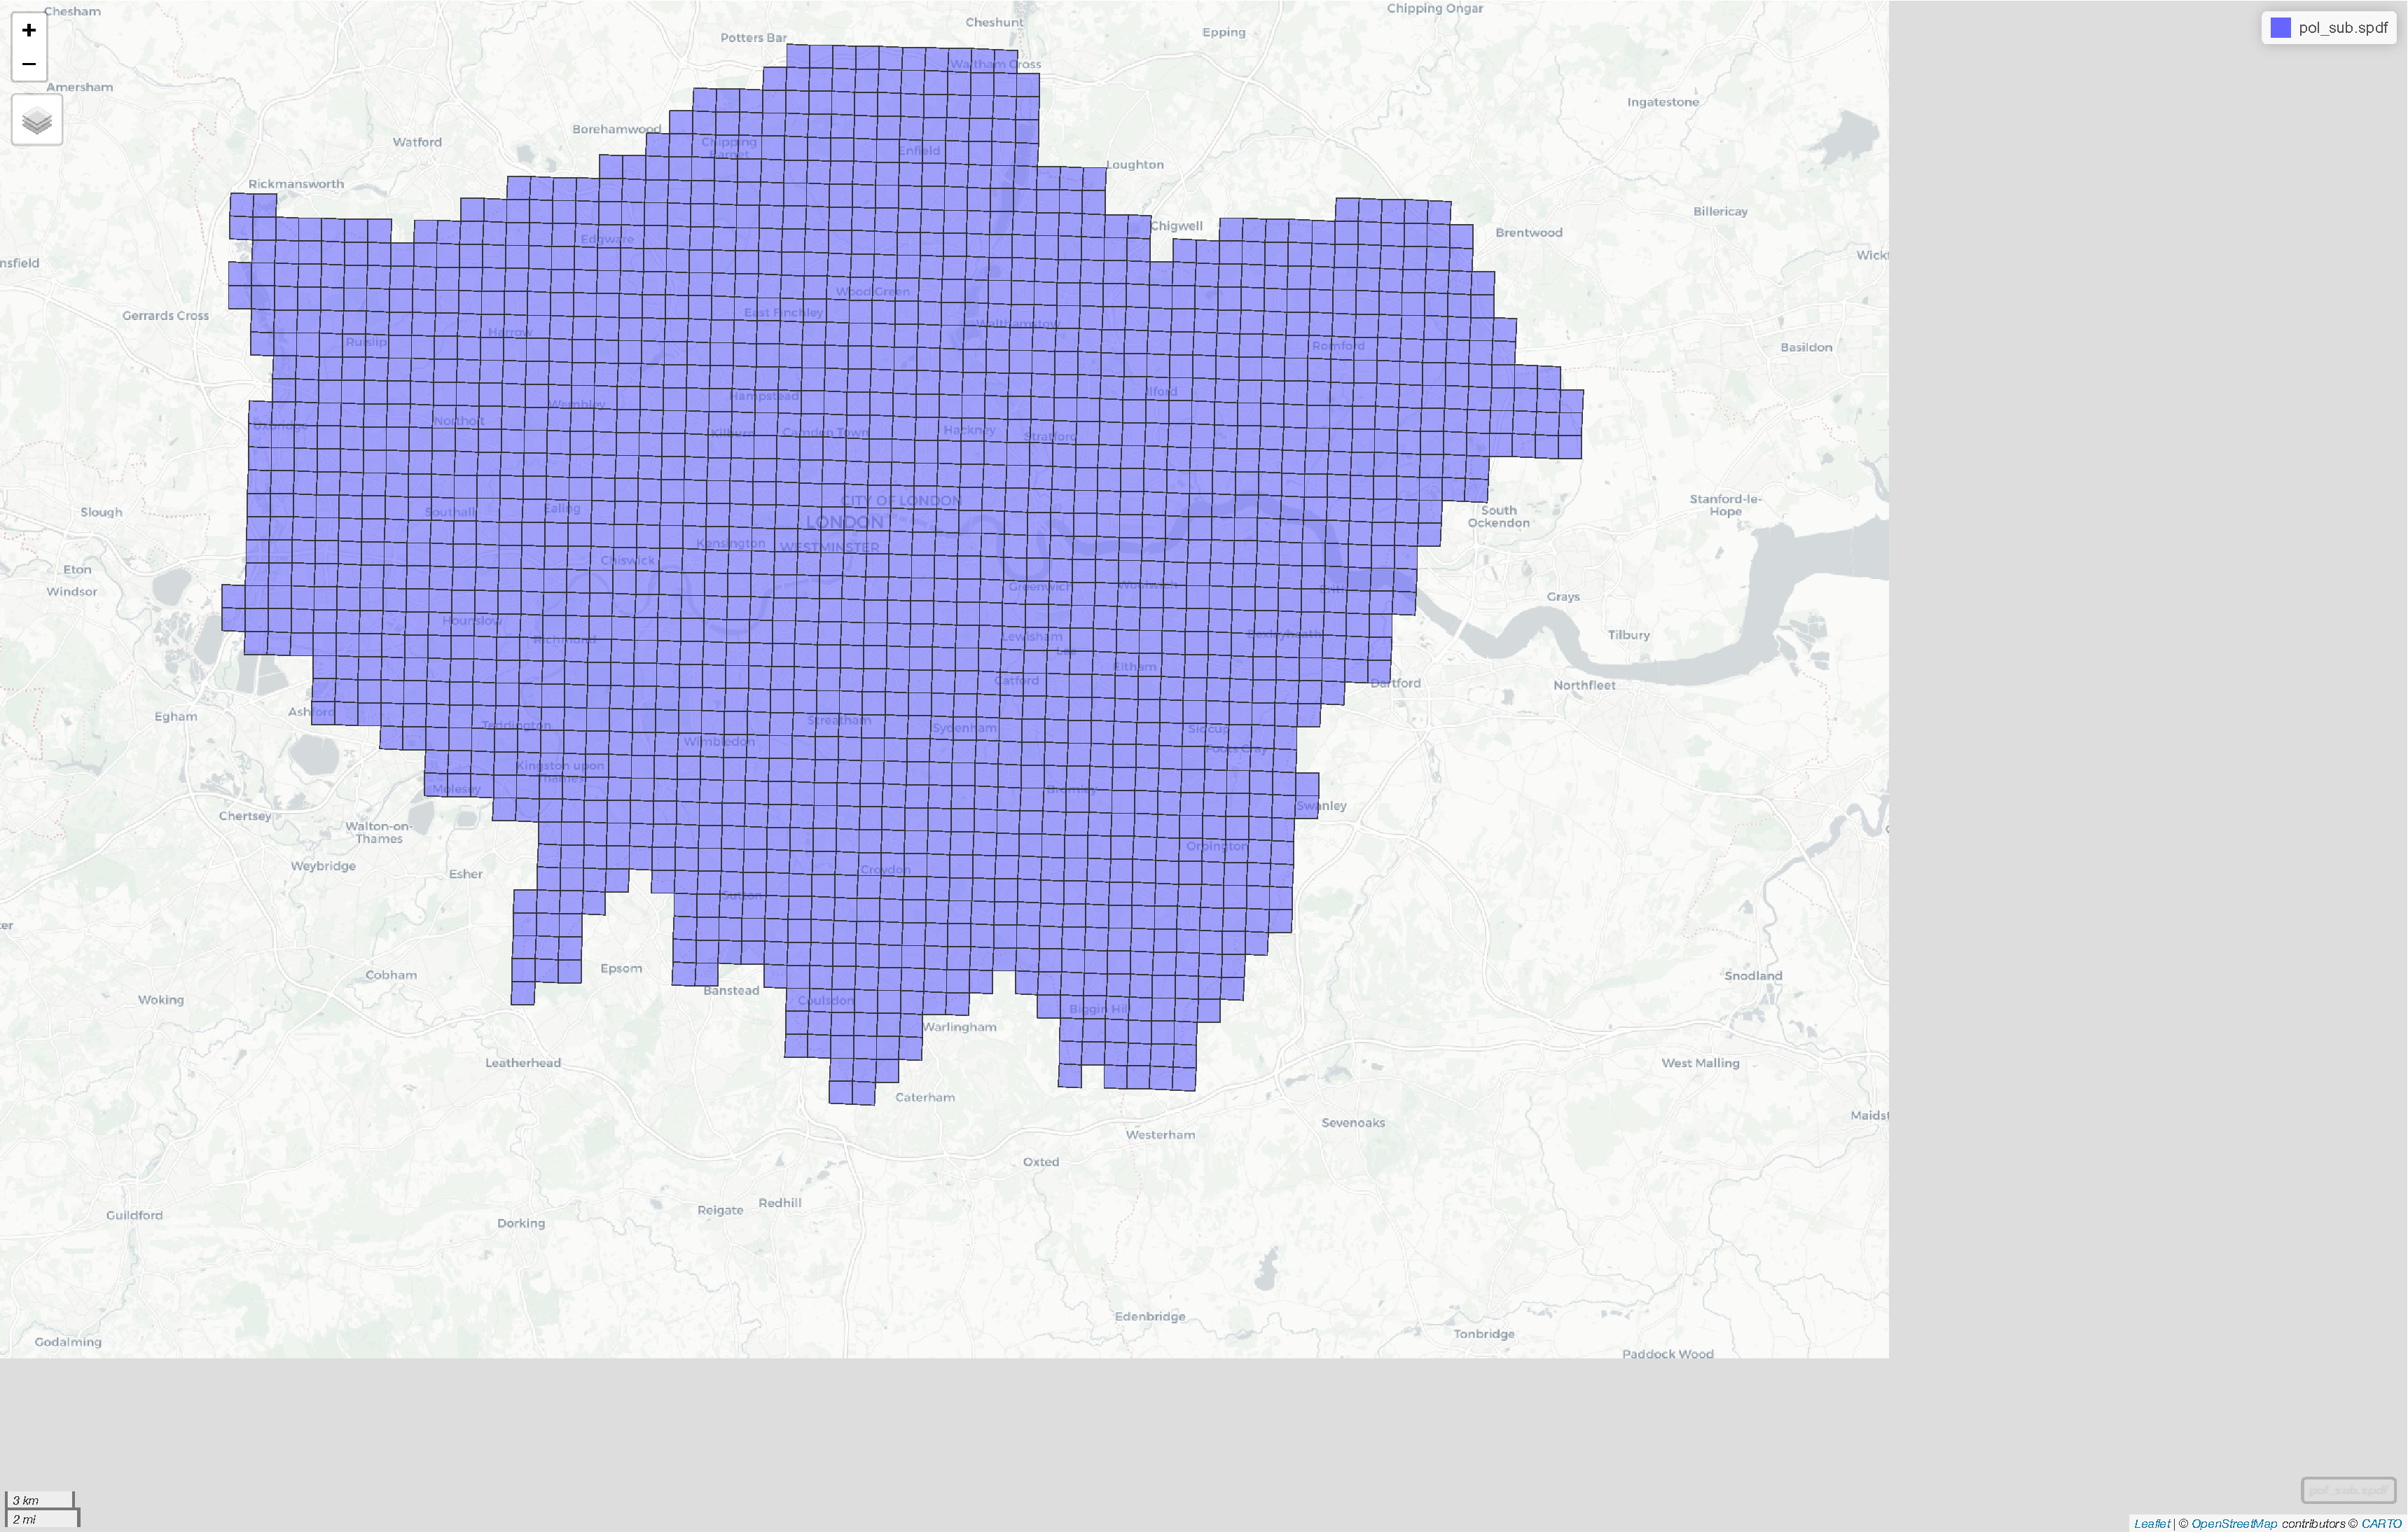
\includegraphics{01_refresher_short_files/figure-pdf/unnamed-chunk-24-1.pdf}

}

\end{figure}

Or we can reverse the above and exclude all intersecting units by
specifying \texttt{st\_disjoint} as alternative spatial operation using
the \texttt{op\ =} option (note the empty space for column selection).
\texttt{st\_filter()} with the \texttt{.predicate} option does the same
job. See the
\href{https://cran.r-project.org/web/packages/sf/vignettes/sf3.html}{sf
Vignette} for more operations.

\begin{Shaded}
\begin{Highlighting}[]
\CommentTok{\# Subset pubs to pubs not in the ulez area}
\NormalTok{sub2.spdf }\OtherTok{\textless{}{-}}\NormalTok{ pubs.spdf[ulez.spdf, , op }\OtherTok{=}\NormalTok{ st\_disjoint] }\CommentTok{\# or:}
\NormalTok{sub2.spdf }\OtherTok{\textless{}{-}} \FunctionTok{st\_filter}\NormalTok{(pubs.spdf, ulez.spdf, }\AttributeTok{.predicate =}\NormalTok{ st\_disjoint)}
\FunctionTok{mapview}\NormalTok{(sub2.spdf)}
\end{Highlighting}
\end{Shaded}

\begin{figure}[H]

{\centering 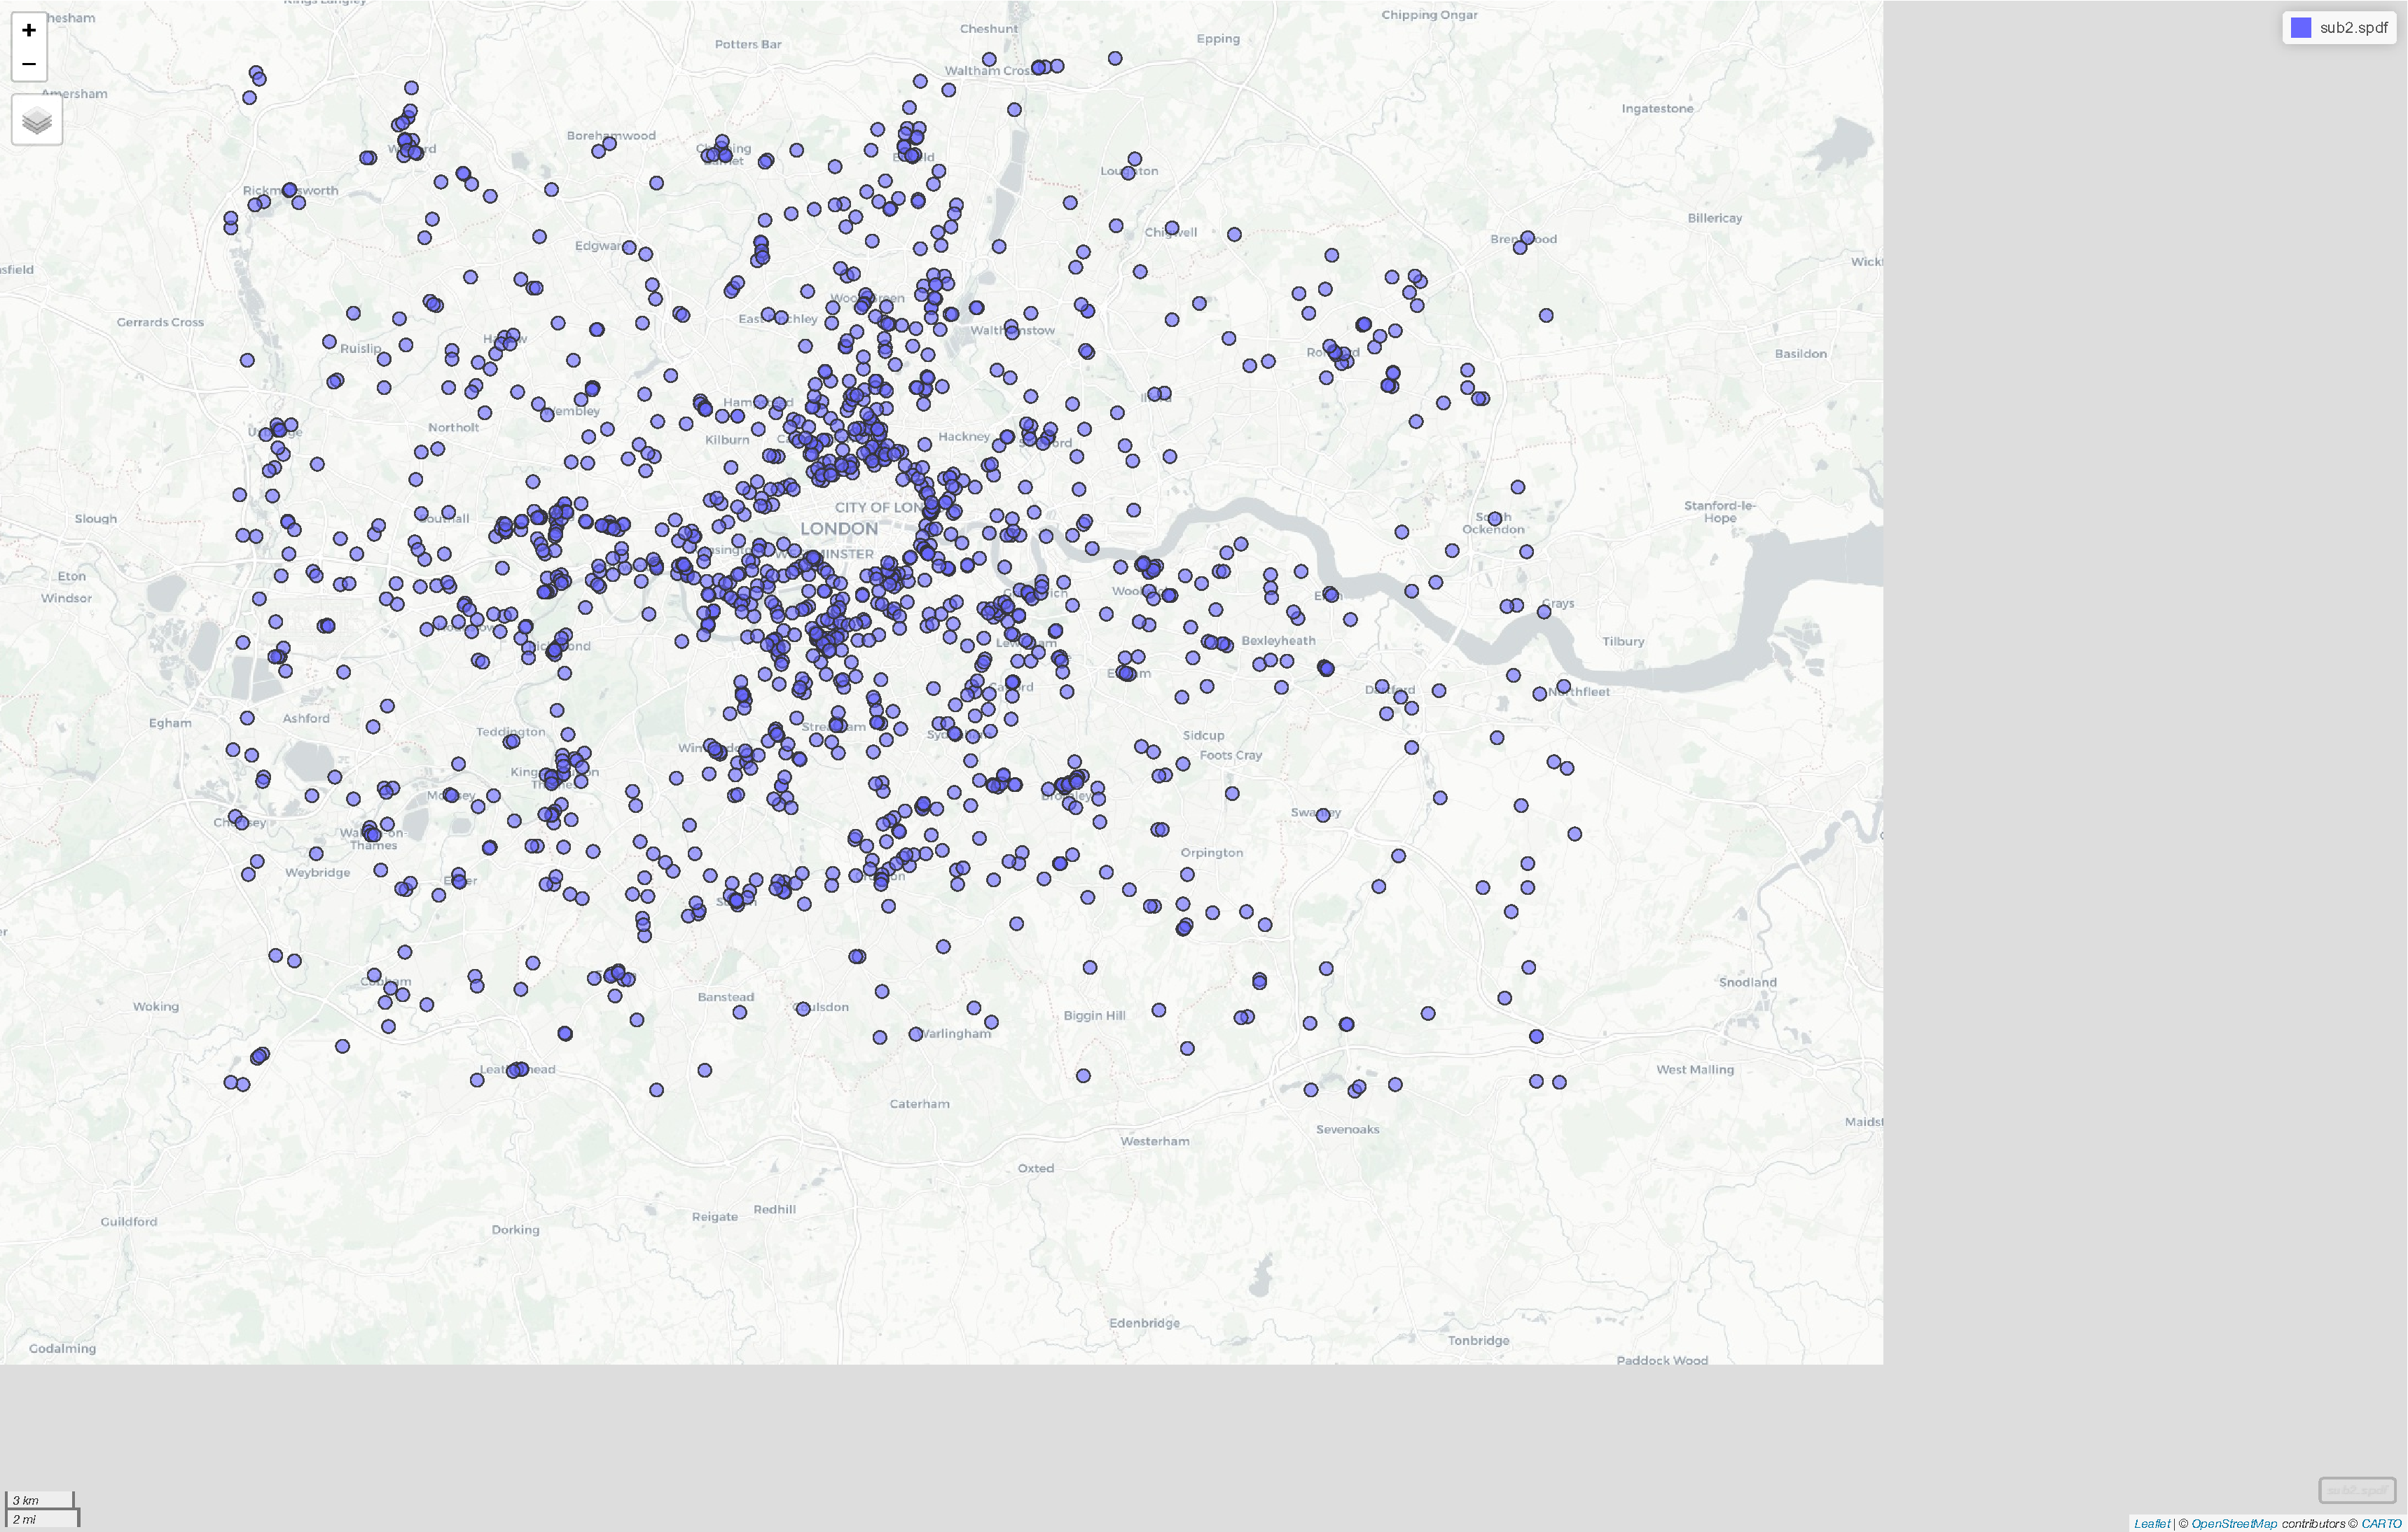
\includegraphics{01_refresher_short_files/figure-pdf/unnamed-chunk-25-1.pdf}

}

\end{figure}

We can easily create indicators of whether an MSOA is within ulez or
not.

\begin{Shaded}
\begin{Highlighting}[]
\NormalTok{msoa.spdf}\SpecialCharTok{$}\NormalTok{ulez }\OtherTok{\textless{}{-}} \DecValTok{0}

\CommentTok{\# intersecting lsoas}
\NormalTok{within }\OtherTok{\textless{}{-}}\NormalTok{ msoa.spdf[ulez.spdf,]}

\CommentTok{\# use their ids to create binary indicator }
\NormalTok{msoa.spdf}\SpecialCharTok{$}\NormalTok{ulez[}\FunctionTok{which}\NormalTok{(msoa.spdf}\SpecialCharTok{$}\NormalTok{MSOA11CD }\SpecialCharTok{\%in\%}\NormalTok{ within}\SpecialCharTok{$}\NormalTok{MSOA11CD)] }\OtherTok{\textless{}{-}} \DecValTok{1}
\FunctionTok{table}\NormalTok{(msoa.spdf}\SpecialCharTok{$}\NormalTok{ulez)}
\end{Highlighting}
\end{Shaded}

\begin{verbatim}

  0   1 
955  28 
\end{verbatim}

\hypertarget{point-in-polygon}{%
\subsection{Point in polygon}\label{point-in-polygon}}

We are interested in the number of pubs in each MSOA. So, we count the
number of points in each polygon.

\begin{Shaded}
\begin{Highlighting}[]
\CommentTok{\# Assign MSOA to each point}
\NormalTok{pubs\_msoa.join }\OtherTok{\textless{}{-}} \FunctionTok{st\_join}\NormalTok{(pubs.spdf, msoa.spdf, }\AttributeTok{join =}\NormalTok{ st\_within)}

\CommentTok{\# Count N by MSOA code (drop geometry to speed up)}
\NormalTok{pubs\_msoa.join }\OtherTok{\textless{}{-}}\NormalTok{ dplyr}\SpecialCharTok{::}\FunctionTok{count}\NormalTok{(}\FunctionTok{st\_drop\_geometry}\NormalTok{(pubs\_msoa.join),}
                               \AttributeTok{MSOA11CD =}\NormalTok{ pubs\_msoa.join}\SpecialCharTok{$}\NormalTok{MSOA11CD,}
                               \AttributeTok{name =} \StringTok{"pubs\_count"}\NormalTok{)}
\FunctionTok{sum}\NormalTok{(pubs\_msoa.join}\SpecialCharTok{$}\NormalTok{pubs\_count)}
\end{Highlighting}
\end{Shaded}

\begin{verbatim}
[1] 1601
\end{verbatim}

\begin{Shaded}
\begin{Highlighting}[]
\CommentTok{\# Merge and replace NAs with zero (no matches, no pubs)}
\NormalTok{msoa.spdf }\OtherTok{\textless{}{-}} \FunctionTok{merge}\NormalTok{(msoa.spdf, pubs\_msoa.join,}
                   \AttributeTok{by =} \StringTok{"MSOA11CD"}\NormalTok{, }\AttributeTok{all.x =} \ConstantTok{TRUE}\NormalTok{)}
\NormalTok{msoa.spdf}\SpecialCharTok{$}\NormalTok{pubs\_count[}\FunctionTok{is.na}\NormalTok{(msoa.spdf}\SpecialCharTok{$}\NormalTok{pubs\_count)] }\OtherTok{\textless{}{-}} \DecValTok{0}
\end{Highlighting}
\end{Shaded}

\hypertarget{distance-measures}{%
\subsection{Distance measures}\label{distance-measures}}

We might be interested in the distance to the nearest pub. Here, we use
the package \texttt{nngeo} to find k nearest neighbours with the
respective distance.

\begin{Shaded}
\begin{Highlighting}[]
\CommentTok{\# Use geometric centroid of each MSOA}
\NormalTok{cent.sp }\OtherTok{\textless{}{-}} \FunctionTok{st\_centroid}\NormalTok{(msoa.spdf[, }\StringTok{"MSOA11CD"}\NormalTok{])}
\end{Highlighting}
\end{Shaded}

\begin{verbatim}
Warning: st_centroid assumes attributes are constant over geometries
\end{verbatim}

\begin{Shaded}
\begin{Highlighting}[]
\CommentTok{\# Get K nearest neighbour with distance}
\NormalTok{knb.dist }\OtherTok{\textless{}{-}} \FunctionTok{st\_nn}\NormalTok{(cent.sp, }
\NormalTok{                  pubs.spdf,}
                  \AttributeTok{k =} \DecValTok{1}\NormalTok{,             }\CommentTok{\# number of nearest neighbours}
                  \AttributeTok{returnDist =} \ConstantTok{TRUE}\NormalTok{, }\CommentTok{\# we also want the distance}
                  \AttributeTok{progress =} \ConstantTok{FALSE}\NormalTok{)}
\end{Highlighting}
\end{Shaded}

\begin{verbatim}
projected points
\end{verbatim}

\begin{Shaded}
\begin{Highlighting}[]
\NormalTok{msoa.spdf}\SpecialCharTok{$}\NormalTok{dist\_pubs }\OtherTok{\textless{}{-}} \FunctionTok{unlist}\NormalTok{(knb.dist}\SpecialCharTok{$}\NormalTok{dist)}
\FunctionTok{summary}\NormalTok{(msoa.spdf}\SpecialCharTok{$}\NormalTok{dist\_pubs)}
\end{Highlighting}
\end{Shaded}

\begin{verbatim}
    Min.  1st Qu.   Median     Mean  3rd Qu.     Max. 
   9.079  305.149  565.018  701.961  948.047 3735.478 
\end{verbatim}

\hypertarget{intersections-buffers}{%
\subsection{Intersections + Buffers}\label{intersections-buffers}}

We may also want the average pollution within 1 km radius around each
MSOA centroid. Note that it is usually better to use a ego-centric
method where you calculate the average within a distance rather than
using the characteristic of the intersecting cells only (Lee et al.
2008; Mohai and Saha 2007).

Therefore, we first create a buffer with \texttt{st\_buffer()} around
each midpoint and subsequently use \texttt{st\_intersetion()} to
calculate the overlap.

\begin{Shaded}
\begin{Highlighting}[]
\CommentTok{\# Create buffer (1km radius)}
\NormalTok{cent.buf }\OtherTok{\textless{}{-}} \FunctionTok{st\_buffer}\NormalTok{(cent.sp, }
                      \AttributeTok{dist =} \DecValTok{1000}\NormalTok{) }\CommentTok{\# dist in meters}
\FunctionTok{mapview}\NormalTok{(cent.buf)}
\end{Highlighting}
\end{Shaded}

\begin{figure}[H]

{\centering 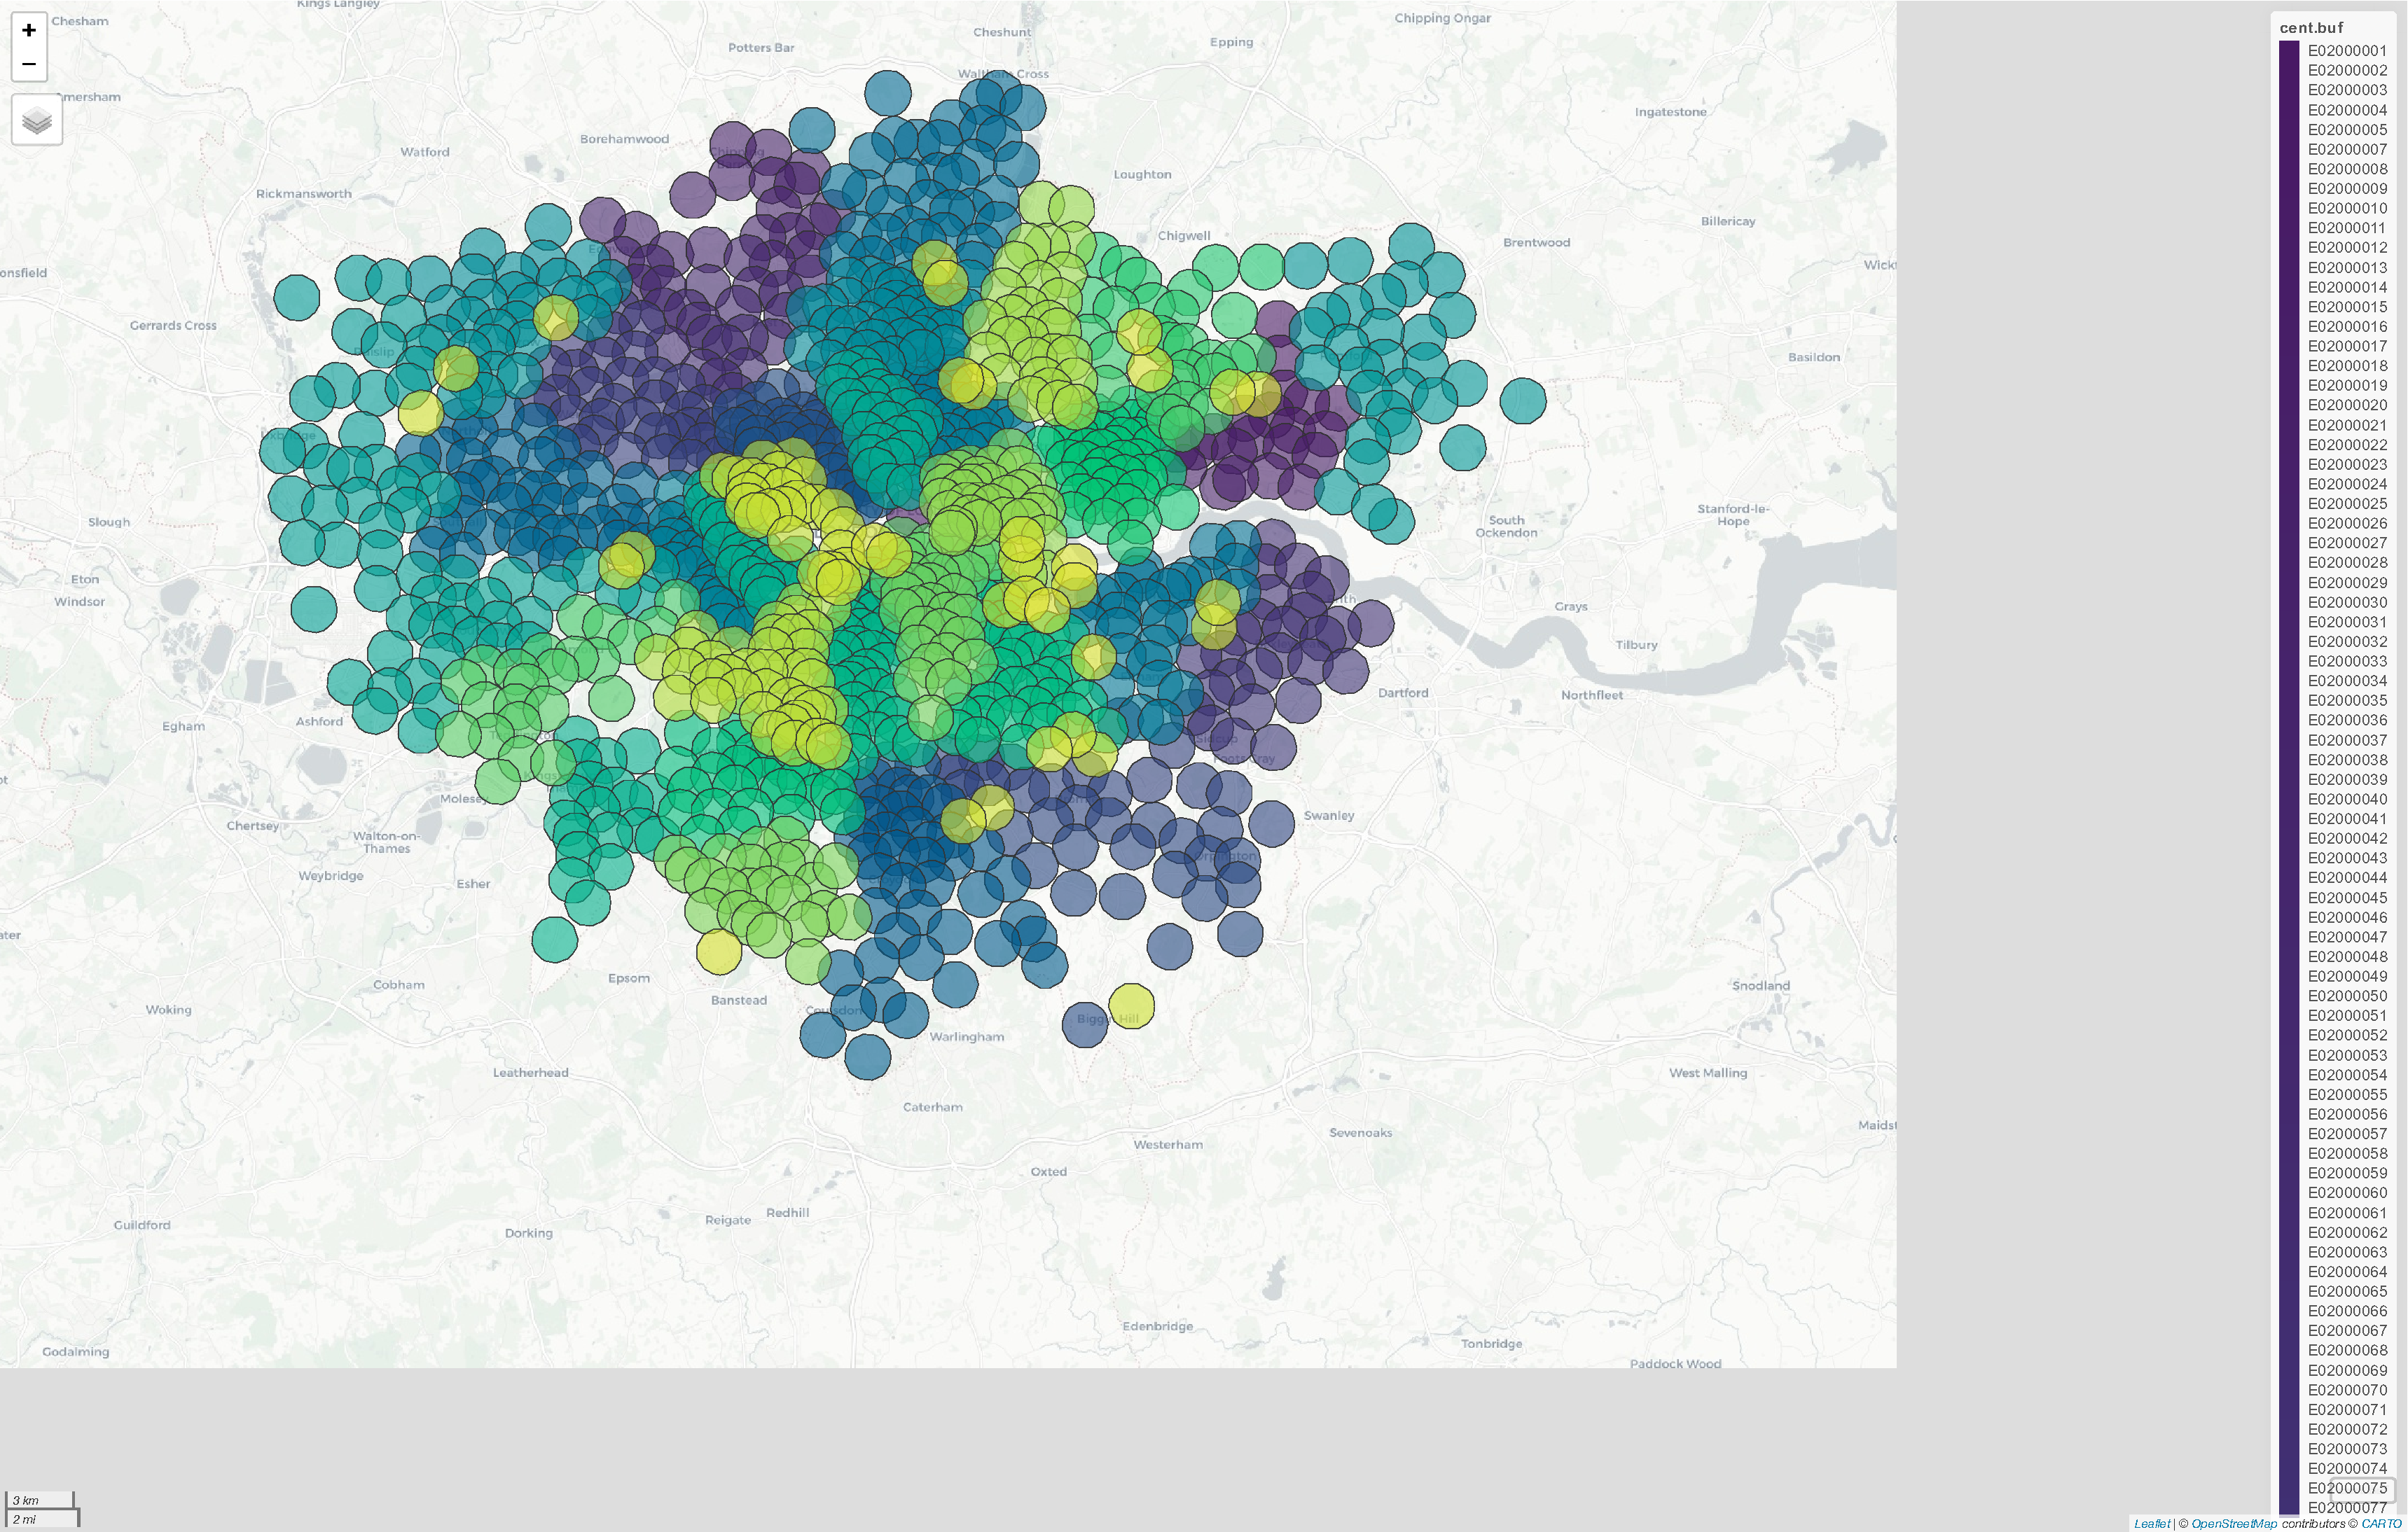
\includegraphics{01_refresher_short_files/figure-pdf/unnamed-chunk-29-1.pdf}

}

\end{figure}

\begin{Shaded}
\begin{Highlighting}[]
\CommentTok{\# Add area of each buffer (in this constant) }
\NormalTok{cent.buf}\SpecialCharTok{$}\NormalTok{area }\OtherTok{\textless{}{-}} \FunctionTok{as.numeric}\NormalTok{(}\FunctionTok{st\_area}\NormalTok{(cent.buf))}

\CommentTok{\# Calculate intersection of pollution grid and buffer}
\NormalTok{int.df }\OtherTok{\textless{}{-}} \FunctionTok{st\_intersection}\NormalTok{(cent.buf, pol.spdf)}
\end{Highlighting}
\end{Shaded}

\begin{verbatim}
Warning: attribute variables are assumed to be spatially constant throughout
all geometries
\end{verbatim}

\begin{Shaded}
\begin{Highlighting}[]
\NormalTok{int.df}\SpecialCharTok{$}\NormalTok{int\_area }\OtherTok{\textless{}{-}} \FunctionTok{as.numeric}\NormalTok{(}\FunctionTok{st\_area}\NormalTok{(int.df)) }\CommentTok{\# area of intersection}

\CommentTok{\# Area of intersection as share of buffer}
\NormalTok{int.df}\SpecialCharTok{$}\NormalTok{area\_per }\OtherTok{\textless{}{-}}\NormalTok{ int.df}\SpecialCharTok{$}\NormalTok{int\_area }\SpecialCharTok{/}\NormalTok{ int.df}\SpecialCharTok{$}\NormalTok{area}
\end{Highlighting}
\end{Shaded}

And we use the percent overalp areas as the weights to calculate a
weighted mean.

\begin{Shaded}
\begin{Highlighting}[]
\CommentTok{\# Aggregate as weighted mean}
\NormalTok{int.df }\OtherTok{\textless{}{-}} \FunctionTok{st\_drop\_geometry}\NormalTok{(int.df)}
\NormalTok{int.df}\SpecialCharTok{$}\NormalTok{no2\_weighted }\OtherTok{\textless{}{-}}\NormalTok{ int.df}\SpecialCharTok{$}\NormalTok{no22011 }\SpecialCharTok{*}\NormalTok{ int.df}\SpecialCharTok{$}\NormalTok{area\_per}
\NormalTok{int.df }\OtherTok{\textless{}{-}} \FunctionTok{aggregate}\NormalTok{(}\FunctionTok{list}\NormalTok{(}\AttributeTok{no2 =}\NormalTok{ int.df[, }\StringTok{"no2\_weighted"}\NormalTok{]), }
                    \AttributeTok{by =} \FunctionTok{list}\NormalTok{(}\AttributeTok{MSOA11CD =}\NormalTok{ int.df}\SpecialCharTok{$}\NormalTok{MSOA11CD),}
\NormalTok{                    sum)}

\CommentTok{\# Merge back to spatial data.frame}
\NormalTok{msoa.spdf }\OtherTok{\textless{}{-}} \FunctionTok{merge}\NormalTok{(msoa.spdf, int.df, }\AttributeTok{by =} \StringTok{"MSOA11CD"}\NormalTok{, }\AttributeTok{all.x =} \ConstantTok{TRUE}\NormalTok{)}

\FunctionTok{mapview}\NormalTok{(msoa.spdf[, }\StringTok{"no2"}\NormalTok{])}
\end{Highlighting}
\end{Shaded}

\begin{figure}[H]

{\centering 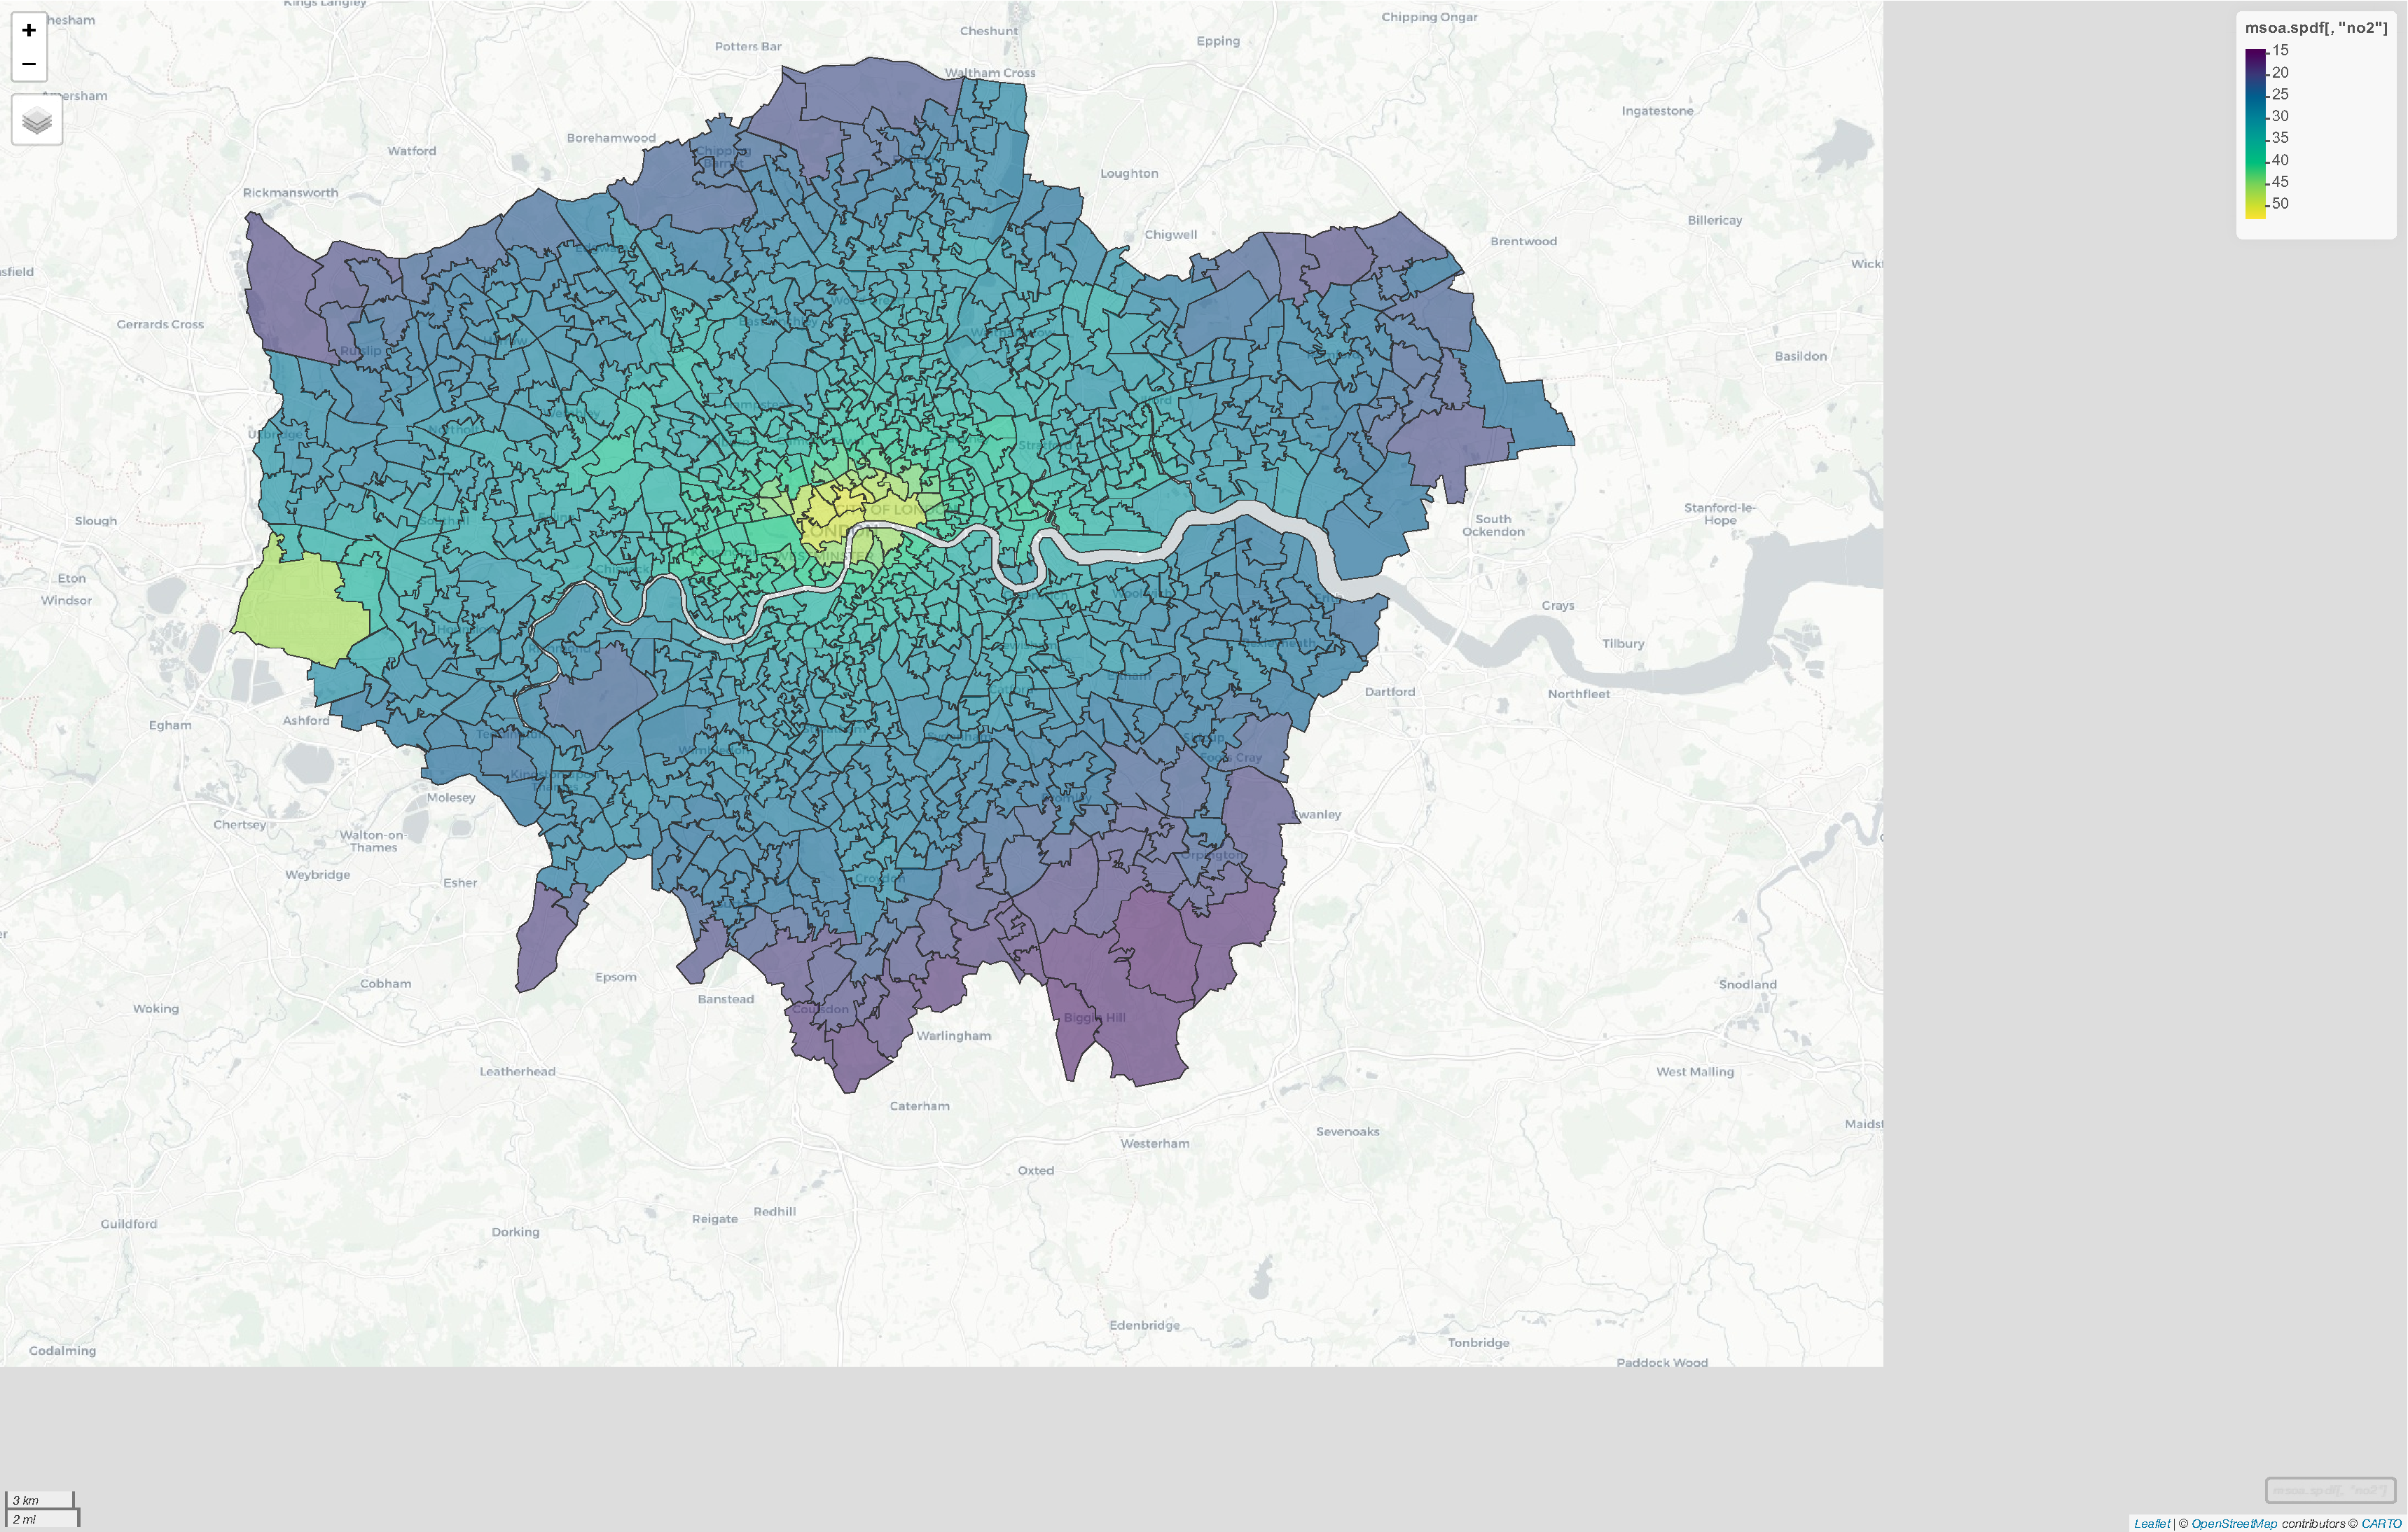
\includegraphics{01_refresher_short_files/figure-pdf/unnamed-chunk-30-1.pdf}

}

\end{figure}

Note: for buffer related methods, it often makes sense to use population
weighted centroids instead of geographic centroids (see
\href{https://geoportal.statistics.gov.uk/datasets/ons::middle-layer-super-output-areas-december-2011-population-weighted-centroids/about}{here}
for MSOA population weighted centroids). However, often this information
is not available.

\hypertarget{and-more}{%
\subsection{and more}\label{and-more}}

There are more spatial operation possible using sf. Have a look at the
\href{fig/sf.pdf}{sf Cheatsheet}.

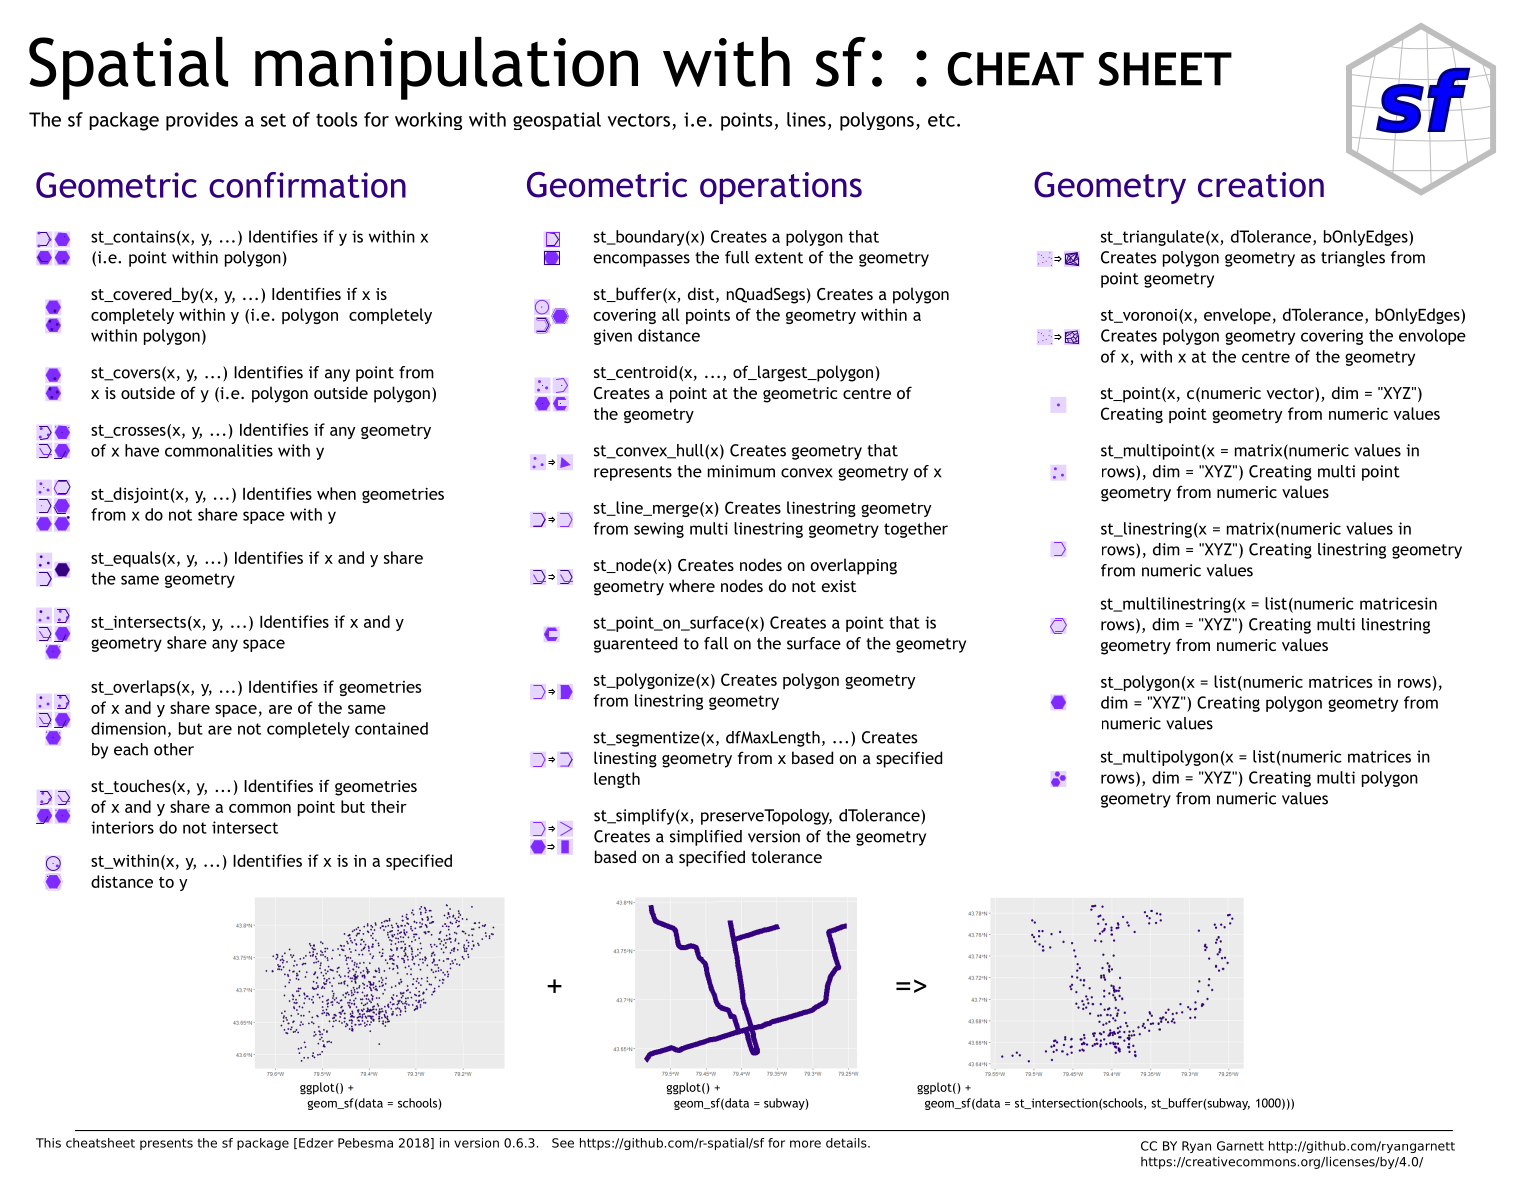
\includegraphics{fig/sf_1.png}

\hypertarget{data-visualisation}{%
\section{Data visualisation}\label{data-visualisation}}

For mapping

\begin{Shaded}
\begin{Highlighting}[]
\NormalTok{pkgs }\OtherTok{\textless{}{-}} \FunctionTok{c}\NormalTok{(}\StringTok{"tmap"}\NormalTok{, }\StringTok{"tmaptools"}\NormalTok{, }\StringTok{"viridisLite"}\NormalTok{, }
          \StringTok{"ggplot2"}\NormalTok{, }\StringTok{"ggthemes"}\NormalTok{, }\StringTok{"rmapshaper"}\NormalTok{) }
\FunctionTok{lapply}\NormalTok{(pkgs, require, }\AttributeTok{character.only =} \ConstantTok{TRUE}\NormalTok{)}
\end{Highlighting}
\end{Shaded}

A large advantage of spatial data is that different data sources can be
connected and combined. Another nice advantage is: you can create very
nice maps. And it's quite easy to do!
\href{https://stefanjuenger.github.io/}{Stefan Jünger} \&
\href{https://www.gesis.org/institut/mitarbeitendenverzeichnis/person/Anne-Kathrin.Stroppe}{Anne-Kathrin
Stroppe} provide more comprehensive materials on mapping in their
\href{https://github.com/StefanJuenger/gesis-workshop-geospatial-techniques-R-2023}{GESIS
workshop on geospatial techniques in R}.

Many packages and functions can be used to plot maps of spatial data.
For instance, ggplot as a function to plot spatial data using
\texttt{geom\_sf()}. I am personally a fan of \texttt{tmap}, which makes
many steps easier (but sometimes is less flexible).

A great tool for choosing coulour is for instance
\href{https://colorbrewer2.org/}{Colorbrewer}. \texttt{viridisLite}
provides another great resource to chose colours.

\hypertarget{tmaps}{%
\subsection{Tmaps}\label{tmaps}}

For instance, lets plot the NO2 estimates using tmap +
\texttt{tm\_fill()} (there are lots of alternatives like
\texttt{tm\_shape}, \texttt{tm\_points()}, \texttt{tm\_dots()}).

\begin{Shaded}
\begin{Highlighting}[]
\CommentTok{\# Define colours}
\NormalTok{cols }\OtherTok{\textless{}{-}} \FunctionTok{viridis}\NormalTok{(}\AttributeTok{n =} \DecValTok{7}\NormalTok{, }\AttributeTok{direction =} \DecValTok{1}\NormalTok{, }\AttributeTok{option =} \StringTok{"C"}\NormalTok{)}

\NormalTok{mp1 }\OtherTok{\textless{}{-}}  \FunctionTok{tm\_shape}\NormalTok{(msoa.spdf) }\SpecialCharTok{+} 
  \FunctionTok{tm\_fill}\NormalTok{(}\AttributeTok{col =} \StringTok{"no2"}\NormalTok{, }
          \AttributeTok{style =} \StringTok{"fisher"}\NormalTok{, }\CommentTok{\# algorithm to def cut points}
          \AttributeTok{n =} \DecValTok{7}\NormalTok{, }\CommentTok{\# Number of requested cut points}
          \AttributeTok{palette =}\NormalTok{ cols, }\CommentTok{\# colours}
          \AttributeTok{alpha =} \DecValTok{1}\NormalTok{, }\CommentTok{\# transparency }
          \AttributeTok{title =} \StringTok{"NO2"}\NormalTok{, }
          \AttributeTok{legend.hist =} \ConstantTok{FALSE} \CommentTok{\# histogram next to map?}
\NormalTok{          ) }\SpecialCharTok{+}
  \FunctionTok{tm\_borders}\NormalTok{(}\AttributeTok{col =} \StringTok{"white"}\NormalTok{, }\AttributeTok{lwd =} \FloatTok{0.5}\NormalTok{, }\AttributeTok{alpha =} \FloatTok{0.5}\NormalTok{) }

\NormalTok{mp1}
\end{Highlighting}
\end{Shaded}

\begin{figure}[H]

{\centering 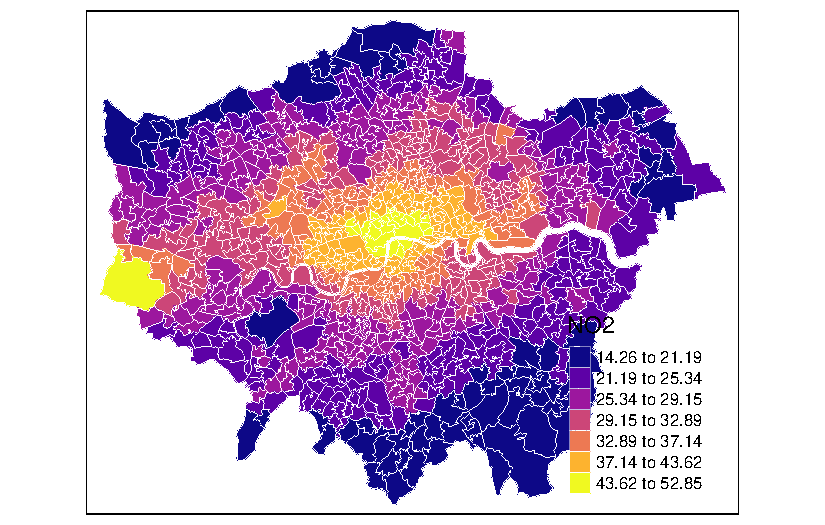
\includegraphics{01_refresher_short_files/figure-pdf/unnamed-chunk-32-1.pdf}

}

\end{figure}

Tmap allows to easily combine different objects by defining a new object
via \texttt{tm\_shape()}.

\begin{Shaded}
\begin{Highlighting}[]
\CommentTok{\# Define colours}
\NormalTok{cols }\OtherTok{\textless{}{-}} \FunctionTok{viridis}\NormalTok{(}\AttributeTok{n =} \DecValTok{7}\NormalTok{, }\AttributeTok{direction =} \DecValTok{1}\NormalTok{, }\AttributeTok{option =} \StringTok{"C"}\NormalTok{)}

\NormalTok{mp1 }\OtherTok{\textless{}{-}}  \FunctionTok{tm\_shape}\NormalTok{(msoa.spdf) }\SpecialCharTok{+} 
  \FunctionTok{tm\_fill}\NormalTok{(}\AttributeTok{col =} \StringTok{"no2"}\NormalTok{, }
          \AttributeTok{style =} \StringTok{"fisher"}\NormalTok{, }\CommentTok{\# algorithm to def cut points}
          \AttributeTok{n =} \DecValTok{7}\NormalTok{, }\CommentTok{\# Number of requested cut points}
          \AttributeTok{palette =}\NormalTok{ cols, }\CommentTok{\# colours}
          \AttributeTok{alpha =} \DecValTok{1}\NormalTok{, }\CommentTok{\# transparency }
          \AttributeTok{title =} \StringTok{"NO2"}\NormalTok{, }
          \AttributeTok{legend.hist =} \ConstantTok{FALSE} \CommentTok{\# histogram next to map?}
\NormalTok{          ) }\SpecialCharTok{+}
  \FunctionTok{tm\_borders}\NormalTok{(}\AttributeTok{col =} \StringTok{"white"}\NormalTok{, }\AttributeTok{lwd =} \FloatTok{0.5}\NormalTok{, }\AttributeTok{alpha =} \FloatTok{0.5}\NormalTok{) }\SpecialCharTok{+}
  \FunctionTok{tm\_shape}\NormalTok{(ulez.spdf) }\SpecialCharTok{+}
  \FunctionTok{tm\_borders}\NormalTok{(}\AttributeTok{col =} \StringTok{"red"}\NormalTok{, }\AttributeTok{lwd =} \DecValTok{1}\NormalTok{, }\AttributeTok{alpha =} \DecValTok{1}\NormalTok{) }

\NormalTok{mp1}
\end{Highlighting}
\end{Shaded}

\begin{figure}[H]

{\centering 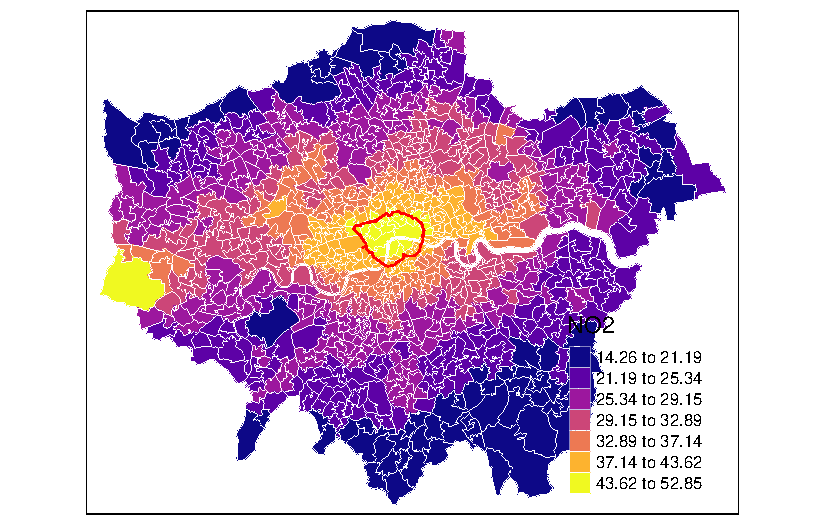
\includegraphics{01_refresher_short_files/figure-pdf/unnamed-chunk-33-1.pdf}

}

\end{figure}

And it is easy to change the layout.

\begin{Shaded}
\begin{Highlighting}[]
\CommentTok{\# Define colours}
\NormalTok{cols }\OtherTok{\textless{}{-}} \FunctionTok{viridis}\NormalTok{(}\AttributeTok{n =} \DecValTok{7}\NormalTok{, }\AttributeTok{direction =} \DecValTok{1}\NormalTok{, }\AttributeTok{option =} \StringTok{"C"}\NormalTok{)}

\NormalTok{mp1 }\OtherTok{\textless{}{-}}  \FunctionTok{tm\_shape}\NormalTok{(msoa.spdf) }\SpecialCharTok{+} 
  \FunctionTok{tm\_fill}\NormalTok{(}\AttributeTok{col =} \StringTok{"no2"}\NormalTok{, }
          \AttributeTok{style =} \StringTok{"fisher"}\NormalTok{, }\CommentTok{\# algorithm to def cut points}
          \AttributeTok{n =} \DecValTok{7}\NormalTok{, }\CommentTok{\# Number of requested cut points}
          \AttributeTok{palette =}\NormalTok{ cols, }\CommentTok{\# colours}
          \AttributeTok{alpha =} \DecValTok{1}\NormalTok{, }\CommentTok{\# transparency }
          \AttributeTok{title =} \FunctionTok{expression}\NormalTok{(}\StringTok{\textquotesingle{}in\textquotesingle{}}\SpecialCharTok{\textasciitilde{}}\NormalTok{mu}\SpecialCharTok{*}\StringTok{\textquotesingle{}g\textquotesingle{}}\SpecialCharTok{/}\NormalTok{m}\SpecialCharTok{\^{}}\NormalTok{\{}\DecValTok{3}\NormalTok{\}), }
          \AttributeTok{legend.hist =} \ConstantTok{FALSE} \CommentTok{\# histogram next to map?}
\NormalTok{          ) }\SpecialCharTok{+}
  \FunctionTok{tm\_borders}\NormalTok{(}\AttributeTok{col =} \StringTok{"white"}\NormalTok{, }\AttributeTok{lwd =} \FloatTok{0.5}\NormalTok{, }\AttributeTok{alpha =} \FloatTok{0.5}\NormalTok{) }\SpecialCharTok{+}
  \FunctionTok{tm\_shape}\NormalTok{(ulez.spdf) }\SpecialCharTok{+}
  \FunctionTok{tm\_borders}\NormalTok{(}\AttributeTok{col =} \StringTok{"red"}\NormalTok{, }\AttributeTok{lwd =} \DecValTok{1}\NormalTok{, }\AttributeTok{alpha =} \DecValTok{1}\NormalTok{) }\SpecialCharTok{+}
  \FunctionTok{tm\_layout}\NormalTok{(}\AttributeTok{frame =} \ConstantTok{FALSE}\NormalTok{,}
            \AttributeTok{legend.frame =} \ConstantTok{TRUE}\NormalTok{, }\AttributeTok{legend.bg.color =} \ConstantTok{TRUE}\NormalTok{,}
            \AttributeTok{legend.position =} \FunctionTok{c}\NormalTok{(}\StringTok{"right"}\NormalTok{, }\StringTok{"bottom"}\NormalTok{),}
            \AttributeTok{legend.outside =} \ConstantTok{FALSE}\NormalTok{,}
            \AttributeTok{main.title =} \StringTok{"NO2"}\NormalTok{, }
            \AttributeTok{main.title.position =} \StringTok{"center"}\NormalTok{,}
            \AttributeTok{main.title.size =} \FloatTok{1.6}\NormalTok{,}
            \AttributeTok{legend.title.size =} \FloatTok{0.8}\NormalTok{,}
            \AttributeTok{legend.text.size =} \FloatTok{0.8}\NormalTok{)}

\NormalTok{mp1}
\end{Highlighting}
\end{Shaded}

\begin{figure}[H]

{\centering 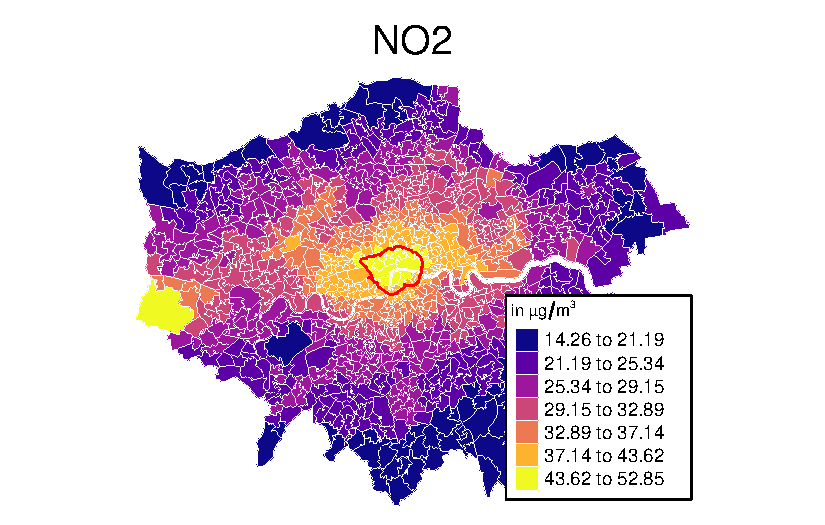
\includegraphics{01_refresher_short_files/figure-pdf/unnamed-chunk-34-1.pdf}

}

\end{figure}

\hypertarget{ggplot}{%
\subsection{ggplot}\label{ggplot}}

For those of you have rather stick with the basic ggplot package, we can
also use ggplot for spatial maps.

\begin{Shaded}
\begin{Highlighting}[]
\NormalTok{gp }\OtherTok{\textless{}{-}} \FunctionTok{ggplot}\NormalTok{(msoa.spdf)}\SpecialCharTok{+}
    \FunctionTok{geom\_sf}\NormalTok{(}\FunctionTok{aes}\NormalTok{(}\AttributeTok{fill =}\NormalTok{ no2))}\SpecialCharTok{+}
    \FunctionTok{scale\_fill\_viridis\_c}\NormalTok{(}\AttributeTok{option =} \StringTok{"B"}\NormalTok{)}\SpecialCharTok{+}
    \FunctionTok{coord\_sf}\NormalTok{(}\AttributeTok{datum =} \ConstantTok{NA}\NormalTok{)}\SpecialCharTok{+}
    \FunctionTok{theme\_map}\NormalTok{()}\SpecialCharTok{+}
    \FunctionTok{theme}\NormalTok{(}\AttributeTok{legend.position =} \FunctionTok{c}\NormalTok{(.}\DecValTok{9}\NormalTok{, .}\DecValTok{6}\NormalTok{))}
\NormalTok{gp}
\end{Highlighting}
\end{Shaded}

\begin{figure}[H]

{\centering 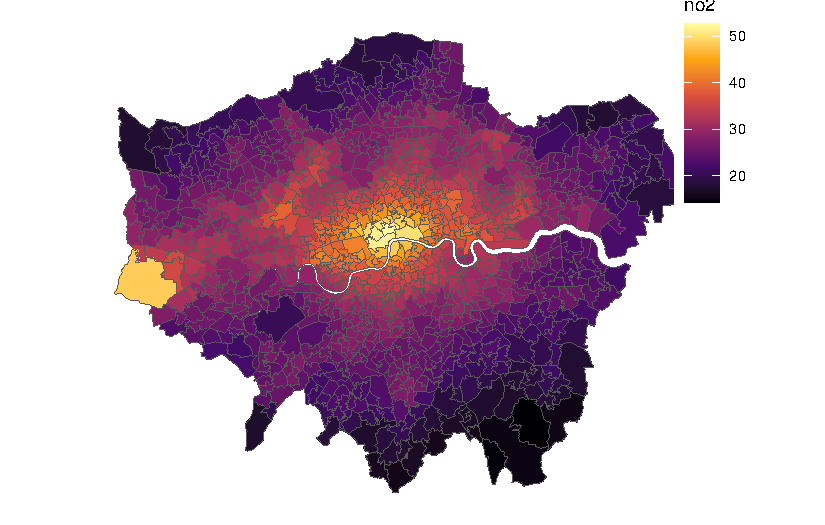
\includegraphics{01_refresher_short_files/figure-pdf/unnamed-chunk-35-1.pdf}

}

\end{figure}

\begin{Shaded}
\begin{Highlighting}[]
\CommentTok{\# Get some larger scale boundaries}
\NormalTok{borough.spdf }\OtherTok{\textless{}{-}} \FunctionTok{st\_read}\NormalTok{(}\AttributeTok{dsn =} \FunctionTok{paste0}\NormalTok{(}\StringTok{"\_data"}\NormalTok{, }\StringTok{"/statistical{-}gis{-}boundaries{-}london/ESRI"}\NormalTok{),}
                     \AttributeTok{layer =} \StringTok{"London\_Borough\_Excluding\_MHW"} \CommentTok{\# Note: no file ending}
\NormalTok{                     )}
\end{Highlighting}
\end{Shaded}

\begin{verbatim}
Reading layer `London_Borough_Excluding_MHW' from data source 
  `C:\work\Lehre\Geodata_Spatial_Regression_short\_data\statistical-gis-boundaries-london\ESRI' 
  using driver `ESRI Shapefile'
Simple feature collection with 33 features and 7 fields
Geometry type: MULTIPOLYGON
Dimension:     XY
Bounding box:  xmin: 503568.2 ymin: 155850.8 xmax: 561957.5 ymax: 200933.9
Projected CRS: OSGB36 / British National Grid
\end{verbatim}

\begin{Shaded}
\begin{Highlighting}[]
\CommentTok{\# transform to only inner lines}
\NormalTok{borough\_inner }\OtherTok{\textless{}{-}} \FunctionTok{ms\_innerlines}\NormalTok{(borough.spdf)}

\CommentTok{\# Plot with inner lines}
\NormalTok{gp }\OtherTok{\textless{}{-}} \FunctionTok{ggplot}\NormalTok{(msoa.spdf)}\SpecialCharTok{+}
    \FunctionTok{geom\_sf}\NormalTok{(}\FunctionTok{aes}\NormalTok{(}\AttributeTok{fill =}\NormalTok{ no2), }\AttributeTok{color =} \ConstantTok{NA}\NormalTok{)}\SpecialCharTok{+}
    \FunctionTok{scale\_fill\_viridis\_c}\NormalTok{(}\AttributeTok{option =} \StringTok{"A"}\NormalTok{)}\SpecialCharTok{+}
    \FunctionTok{geom\_sf}\NormalTok{(}\AttributeTok{data =}\NormalTok{ borough\_inner, }\AttributeTok{color =} \StringTok{"gray92"}\NormalTok{)}\SpecialCharTok{+}
    \FunctionTok{geom\_sf}\NormalTok{(}\AttributeTok{data =}\NormalTok{ ulez.spdf, }\AttributeTok{color =} \StringTok{"red"}\NormalTok{, }\AttributeTok{fill =} \ConstantTok{NA}\NormalTok{)}\SpecialCharTok{+}
    \FunctionTok{coord\_sf}\NormalTok{(}\AttributeTok{datum =} \ConstantTok{NA}\NormalTok{)}\SpecialCharTok{+}
    \FunctionTok{theme\_map}\NormalTok{()}\SpecialCharTok{+}
    \FunctionTok{labs}\NormalTok{(}\AttributeTok{fill =} \StringTok{"NO2"}\NormalTok{)}\SpecialCharTok{+}
    \FunctionTok{theme}\NormalTok{(}\AttributeTok{legend.position =} \FunctionTok{c}\NormalTok{(.}\DecValTok{9}\NormalTok{, .}\DecValTok{6}\NormalTok{))}
\NormalTok{gp}
\end{Highlighting}
\end{Shaded}

\begin{figure}[H]

{\centering 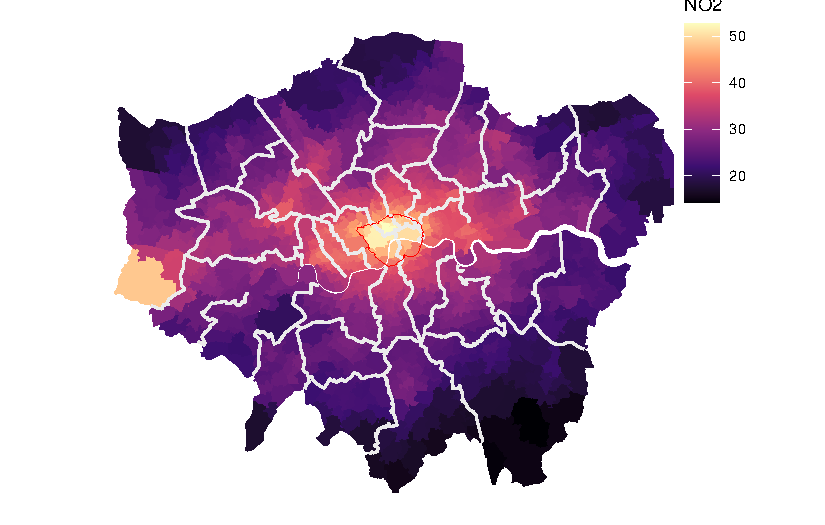
\includegraphics{01_refresher_short_files/figure-pdf/unnamed-chunk-36-1.pdf}

}

\end{figure}

\hypertarget{exercise}{%
\section{Exercise}\label{exercise}}

\begin{enumerate}
\def\labelenumi{\arabic{enumi})}
\item
  What is the difference between a spatial ``sf'' object and a
  conventional ``data.frame''? What's the purpose of the function
  \texttt{st\_drop\_geometry()}?
\item
  Using msoa.spdf, please create a spatial data frame that contains only
  the MSOA areas that are within the ulez zone.
\item
  Please create a map for London (or only the msoa-ulez subset) which
  shows the share of Asian residents (or any other ethnic group).
\item
  Please calculate the distance of each MSOA to the London city centre
\end{enumerate}

\begin{enumerate}
\def\labelenumi{\alph{enumi})}
\tightlist
\item
  use google maps to get lon and lat,
\item
  us \texttt{st\_as\_sf()} to create the spatial point
\item
  use \texttt{st\_distance()} to calculate the distance
\end{enumerate}

\begin{enumerate}
\def\labelenumi{\arabic{enumi})}
\setcounter{enumi}{4}
\tightlist
\item
  Can you create a plot with the distance to the city centre and pub
  counts next to each other?
\end{enumerate}

\bookmarksetup{startatroot}

\hypertarget{references}{%
\chapter*{References}\label{references}}
\addcontentsline{toc}{chapter}{References}

\markboth{References}{References}

\hypertarget{refs}{}
\begin{CSLReferences}{1}{0}
\leavevmode\vadjust pre{\hypertarget{ref-Appelhans.2021}{}}%
Appelhans, Tim, Florian Detsch, Chritoph Reudenbach, and Stefan
Woellauer. 2021. {``Mapview: {Interactive Viewing} of {Spatial Data} in
{R}.''}

\leavevmode\vadjust pre{\hypertarget{ref-Bivand.2018}{}}%
Bivand, Roger S., and Colin Rudel. 2018. {``Rgeos: {Interface} to
{Geometry Engine} - {Open Source} ('{GEOS}').''}

\leavevmode\vadjust pre{\hypertarget{ref-Bivand.2021}{}}%
Bivand, Roger, Giovanni Millo, and Gianfranco Piras. 2021. {``A {Review}
of {Software} for {Spatial Econometrics} in {R}.''} \emph{Mathematics} 9
(11): 1276. \url{https://doi.org/10.3390/math9111276}.

\leavevmode\vadjust pre{\hypertarget{ref-Bivand.2015}{}}%
Bivand, Roger, and Gianfranco Piras. 2015. {``Comparing
{Implementations} of {Estimation Methods} for {Spatial Econometrics}.''}
\emph{Journal of Statistical Software} 63 (18): 1--36.
\url{https://doi.org/10.18637/jss.v063.i18}.

\leavevmode\vadjust pre{\hypertarget{ref-Elhorst.2012}{}}%
Elhorst, J. Paul. 2012. {``Dynamic Spatial Panels: Models, Methods, and
Inferences.''} \emph{Journal of Geographical Systems} 14 (1): 5--28.
\url{https://doi.org/10.1007/s10109-011-0158-4}.

\leavevmode\vadjust pre{\hypertarget{ref-Graler.2016}{}}%
Gräler, Benedikt, Edzer Pebesma, and Gerard Heuvelink. 2016.
{``Spatio-{Temporal Interpolation} Using Gstat.''} \emph{The R Journal}
8 (1): 204--18.

\leavevmode\vadjust pre{\hypertarget{ref-HalleckVega.2015}{}}%
Halleck Vega, Solmaria, and J. Paul Elhorst. 2015. {``The {SLX
Model}.''} \emph{Journal of Regional Science} 55 (3): 339--63.
\url{https://doi.org/10.1111/jors.12188}.

\leavevmode\vadjust pre{\hypertarget{ref-Lee.2008}{}}%
Lee, Barrett A., Sean F. Reardon, Glenn Firebaugh, Chad R. Farrell,
Stephen A. Matthews, and David O'Sullivan. 2008. {``Beyond the {Census
Tract}: {Patterns} and {Determinants} of {Racial Segregation} at
{Multiple Geographic Scales}.''} \emph{American Sociological Review} 73
(5): 766--91. \url{https://doi.org/10.1177/000312240807300504}.

\leavevmode\vadjust pre{\hypertarget{ref-LeSage.2014}{}}%
LeSage, James P. 2014. {``What {Regional Scientists Need} to {Know}
about {Spatial Econometrics}.''} \emph{The Review of Regional Studies}
44 (1): 13--32.
https://doi.org/\url{https://dx.doi.org/10.2139/ssrn.2420725}.

\leavevmode\vadjust pre{\hypertarget{ref-LeSage.2009}{}}%
LeSage, James P., and R. Kelley Pace. 2009. \emph{Introduction to
{Spatial Econometrics}}. Statistics, {Textbooks} and {Monographs}. {Boca
Raton}: {CRC Press}.

\leavevmode\vadjust pre{\hypertarget{ref-Lovelace.2019}{}}%
Lovelace, Robin, Jakub Nowosad, and Jannes Muenchow. 2019.
\emph{Geocomputation with {R}}. 1st ed. Chapman \& {Hall}/{CRC} the {R}
Series. {Boca Raton}: {Chapman \& Hall/CRC}.

\leavevmode\vadjust pre{\hypertarget{ref-Mohai.2007}{}}%
Mohai, Paul, and Robin Saha. 2007. {``Racial {Inequality} in the
{Distribution} of {Hazardous Waste}: {A National-Level Reassessment}.''}
\emph{Social Problems} 54 (3): 343--70.
\url{https://doi.org/10.1525/sp.2007.54.3.343}.

\leavevmode\vadjust pre{\hypertarget{ref-Pebesma.2018}{}}%
Pebesma, Edzer. 2018. {``Simple Features for {R}: {Standardized} Support
for Spatial Vector Data.''} \emph{The R Journal} 10 (1): 439.
\url{https://doi.org/10.32614/RJ-2018-009}.

\leavevmode\vadjust pre{\hypertarget{ref-Pebesma.2023}{}}%
Pebesma, Edzer, and Roger Bivand. 2023. \emph{Spatial {Data Science}:
{With Applications} in {R}}. First. {Boca Raton}: {Chapman and
Hall/CRC}. \url{https://doi.org/10.1201/9780429459016}.

\leavevmode\vadjust pre{\hypertarget{ref-Ruttenauer.2022a}{}}%
Rüttenauer, Tobias. 2022. {``Spatial {Regression Models}: {A Systematic
Comparison} of {Different Model Specifications Using Monte Carlo
Experiments}.''} \emph{Sociological Methods \& Research} 51 (2):
728--59. \url{https://doi.org/10.1177/0049124119882467}.

\leavevmode\vadjust pre{\hypertarget{ref-Ruttenauer.2024b}{}}%
---------. 2024. {``Spatial {Data Analysis}.''} {arXiv}.
\url{https://arxiv.org/abs/2402.09895}.

\leavevmode\vadjust pre{\hypertarget{ref-Tennekes.2018}{}}%
Tennekes, Martijn. 2018. {``Tmap : {Thematic Maps} in {R}.''}
\emph{Journal of Statistical Software} 84 (6).
\url{https://doi.org/10.18637/jss.v084.i06}.

\leavevmode\vadjust pre{\hypertarget{ref-Ward.2008}{}}%
Ward, Michael Don, and Kristian Skrede Gleditsch. 2008. \emph{Spatial
{Regression Models}}. Vol. 155. Quantitative {Applications} in the
{Social Sciences}. {Thousand Oaks}: {Sage}.

\end{CSLReferences}



\end{document}
